% Options for packages loaded elsewhere
% Options for packages loaded elsewhere
\PassOptionsToPackage{unicode}{hyperref}
\PassOptionsToPackage{hyphens}{url}
\PassOptionsToPackage{dvipsnames,svgnames,x11names}{xcolor}
%
\documentclass[
  spanish,
  a4paper,
  12pt,
  twoside]{memoir}
\usepackage{xcolor}
\usepackage{amsmath,amssymb}
\setcounter{secnumdepth}{5}
\usepackage{iftex}
\ifPDFTeX
  \usepackage[T1]{fontenc}
  \usepackage[utf8]{inputenc}
  \usepackage{textcomp} % provide euro and other symbols
\else % if luatex or xetex
  \usepackage{unicode-math} % this also loads fontspec
  \defaultfontfeatures{Scale=MatchLowercase}
  \defaultfontfeatures[\rmfamily]{Ligatures=TeX,Scale=1}
\fi
\usepackage{lmodern}
\ifPDFTeX\else
  % xetex/luatex font selection
\fi
% Use upquote if available, for straight quotes in verbatim environments
\IfFileExists{upquote.sty}{\usepackage{upquote}}{}
\IfFileExists{microtype.sty}{% use microtype if available
  \usepackage[]{microtype}
  \UseMicrotypeSet[protrusion]{basicmath} % disable protrusion for tt fonts
}{}
\makeatletter
\@ifundefined{KOMAClassName}{% if non-KOMA class
  \IfFileExists{parskip.sty}{%
    \usepackage{parskip}
  }{% else
    \setlength{\parindent}{0pt}
    \setlength{\parskip}{6pt plus 2pt minus 1pt}}
}{% if KOMA class
  \KOMAoptions{parskip=half}}
\makeatother
% Make \paragraph and \subparagraph free-standing
\makeatletter
\ifx\paragraph\undefined\else
  \let\oldparagraph\paragraph
  \renewcommand{\paragraph}{
    \@ifstar
      \xxxParagraphStar
      \xxxParagraphNoStar
  }
  \newcommand{\xxxParagraphStar}[1]{\oldparagraph*{#1}\mbox{}}
  \newcommand{\xxxParagraphNoStar}[1]{\oldparagraph{#1}\mbox{}}
\fi
\ifx\subparagraph\undefined\else
  \let\oldsubparagraph\subparagraph
  \renewcommand{\subparagraph}{
    \@ifstar
      \xxxSubParagraphStar
      \xxxSubParagraphNoStar
  }
  \newcommand{\xxxSubParagraphStar}[1]{\oldsubparagraph*{#1}\mbox{}}
  \newcommand{\xxxSubParagraphNoStar}[1]{\oldsubparagraph{#1}\mbox{}}
\fi
\makeatother

\usepackage{color}
\usepackage{fancyvrb}
\newcommand{\VerbBar}{|}
\newcommand{\VERB}{\Verb[commandchars=\\\{\}]}
\DefineVerbatimEnvironment{Highlighting}{Verbatim}{commandchars=\\\{\}}
% Add ',fontsize=\small' for more characters per line
\usepackage{framed}
\definecolor{shadecolor}{RGB}{241,243,245}
\newenvironment{Shaded}{\begin{snugshade}}{\end{snugshade}}
\newcommand{\AlertTok}[1]{\textcolor[rgb]{0.68,0.00,0.00}{#1}}
\newcommand{\AnnotationTok}[1]{\textcolor[rgb]{0.37,0.37,0.37}{#1}}
\newcommand{\AttributeTok}[1]{\textcolor[rgb]{0.40,0.45,0.13}{#1}}
\newcommand{\BaseNTok}[1]{\textcolor[rgb]{0.68,0.00,0.00}{#1}}
\newcommand{\BuiltInTok}[1]{\textcolor[rgb]{0.00,0.23,0.31}{#1}}
\newcommand{\CharTok}[1]{\textcolor[rgb]{0.13,0.47,0.30}{#1}}
\newcommand{\CommentTok}[1]{\textcolor[rgb]{0.37,0.37,0.37}{#1}}
\newcommand{\CommentVarTok}[1]{\textcolor[rgb]{0.37,0.37,0.37}{\textit{#1}}}
\newcommand{\ConstantTok}[1]{\textcolor[rgb]{0.56,0.35,0.01}{#1}}
\newcommand{\ControlFlowTok}[1]{\textcolor[rgb]{0.00,0.23,0.31}{\textbf{#1}}}
\newcommand{\DataTypeTok}[1]{\textcolor[rgb]{0.68,0.00,0.00}{#1}}
\newcommand{\DecValTok}[1]{\textcolor[rgb]{0.68,0.00,0.00}{#1}}
\newcommand{\DocumentationTok}[1]{\textcolor[rgb]{0.37,0.37,0.37}{\textit{#1}}}
\newcommand{\ErrorTok}[1]{\textcolor[rgb]{0.68,0.00,0.00}{#1}}
\newcommand{\ExtensionTok}[1]{\textcolor[rgb]{0.00,0.23,0.31}{#1}}
\newcommand{\FloatTok}[1]{\textcolor[rgb]{0.68,0.00,0.00}{#1}}
\newcommand{\FunctionTok}[1]{\textcolor[rgb]{0.28,0.35,0.67}{#1}}
\newcommand{\ImportTok}[1]{\textcolor[rgb]{0.00,0.46,0.62}{#1}}
\newcommand{\InformationTok}[1]{\textcolor[rgb]{0.37,0.37,0.37}{#1}}
\newcommand{\KeywordTok}[1]{\textcolor[rgb]{0.00,0.23,0.31}{\textbf{#1}}}
\newcommand{\NormalTok}[1]{\textcolor[rgb]{0.00,0.23,0.31}{#1}}
\newcommand{\OperatorTok}[1]{\textcolor[rgb]{0.37,0.37,0.37}{#1}}
\newcommand{\OtherTok}[1]{\textcolor[rgb]{0.00,0.23,0.31}{#1}}
\newcommand{\PreprocessorTok}[1]{\textcolor[rgb]{0.68,0.00,0.00}{#1}}
\newcommand{\RegionMarkerTok}[1]{\textcolor[rgb]{0.00,0.23,0.31}{#1}}
\newcommand{\SpecialCharTok}[1]{\textcolor[rgb]{0.37,0.37,0.37}{#1}}
\newcommand{\SpecialStringTok}[1]{\textcolor[rgb]{0.13,0.47,0.30}{#1}}
\newcommand{\StringTok}[1]{\textcolor[rgb]{0.13,0.47,0.30}{#1}}
\newcommand{\VariableTok}[1]{\textcolor[rgb]{0.07,0.07,0.07}{#1}}
\newcommand{\VerbatimStringTok}[1]{\textcolor[rgb]{0.13,0.47,0.30}{#1}}
\newcommand{\WarningTok}[1]{\textcolor[rgb]{0.37,0.37,0.37}{\textit{#1}}}

\usepackage{longtable,booktabs,array}
\newcounter{none} % for unnumbered tables
\usepackage{calc} % for calculating minipage widths
% Correct order of tables after \paragraph or \subparagraph
\usepackage{etoolbox}
\makeatletter
\patchcmd\longtable{\par}{\if@noskipsec\mbox{}\fi\par}{}{}
\makeatother
% Allow footnotes in longtable head/foot
\IfFileExists{footnotehyper.sty}{\usepackage{footnotehyper}}{\usepackage{footnote}}
\makesavenoteenv{longtable}
\usepackage{graphicx}
\makeatletter
\newsavebox\pandoc@box
\newcommand*\pandocbounded[1]{% scales image to fit in text height/width
  \sbox\pandoc@box{#1}%
  \Gscale@div\@tempa{\textheight}{\dimexpr\ht\pandoc@box+\dp\pandoc@box\relax}%
  \Gscale@div\@tempb{\linewidth}{\wd\pandoc@box}%
  \ifdim\@tempb\p@<\@tempa\p@\let\@tempa\@tempb\fi% select the smaller of both
  \ifdim\@tempa\p@<\p@\scalebox{\@tempa}{\usebox\pandoc@box}%
  \else\usebox{\pandoc@box}%
  \fi%
}
% Set default figure placement to htbp
\def\fps@figure{htbp}
\makeatother



\ifLuaTeX
\usepackage[bidi=basic,shorthands=off]{babel}
\else
\usepackage[bidi=default,shorthands=off]{babel}
\fi
\ifLuaTeX
  \usepackage{selnolig} % disable illegal ligatures
\fi


\setlength{\emergencystretch}{3em} % prevent overfull lines

\providecommand{\tightlist}{%
  \setlength{\itemsep}{0pt}\setlength{\parskip}{0pt}}



 
\usepackage[]{natbib}
\bibliographystyle{apalike}


%% ============================================================
%%  Preámbulo LaTeX – Anexos TFG GIS UBU
%%  Mismo contenido que preambulo_memoria.tex; se mantiene
%%  separado para facilitar ajustes independientes.
%% ============================================================

%\usepackage[spanish,es-tabla]{babel} % No es necesario en Quarto
%\selectlanguage{spanish} % No es necesario en Quarto
\addto\captionsspanish{\renewcommand{\tablename}{Tabla}}
\addto\captionsspanish{\renewcommand{\listtablename}{Índice de tablas}}
\addto\captionsspanish{\renewcommand{\contentsname}{Índice general}}
\addto\captionsspanish{\renewcommand{\listfigurename}{Índice de figuras}}


\usepackage{lmodern}
\usepackage{microtype}
\usepackage{placeins}

\RequirePackage{booktabs}
%\RequirePackage[table]{xcolor}
\PassOptionsToPackage{table}{xcolor}
\RequirePackage{xtab}
\RequirePackage{multirow}
\RequirePackage{tabularx}

\PassOptionsToPackage{hyphens}{url}
\usepackage[colorlinks]{hyperref}
\hypersetup{allcolors={red}}

\usepackage{amsmath}

\nonzeroparskip
\widowpenalty100000
\clubpenalty100000
\nouppercaseheads

\let\tmp\oddsidemargin
\let\oddsidemargin\evensidemargin
\let\evensidemargin\tmp
\reversemarginpar

\usepackage{graphicx}
\graphicspath{{./img/}}

\newcommand{\imagen}[3]{%
  \begin{figure}[!h]
    \centering
    \includegraphics[width=#3\textwidth]{#1}
    \caption{#2}\label{fig:#1}
  \end{figure}
  \FloatBarrier
}

\newcommand{\ruta}[1]{{\sffamily #1}}

\chapterstyle{bianchi}

%% Para los anexos NO se usa \capitulo; se usa \apendice
\renewcommand{\appendixname}{Apéndice}
\renewcommand*\cftappendixname{\appendixname}
\newcommand{\apendice}[1]{\chapter{#1}}
\renewcommand*\cftappendixname{\appendixname\ }

\usepackage{xcolor}
\definecolor{newBox}{HTML}{D8AD6E}

\makeatletter
\newcommand{\tutor}[1]{\def\@tutor{#1}}
\newcommand{\tutorb}[1]{\def\@tutorb{#1}}
\newcommand{\tutorc}[1]{\def\@tutorc{#1}}
\newcommand{\course}[1]{\def\@course{#1}}

% ── EDITAR ESTOS DATOS ──────────────────────────────────────
\newcommand{\nombre}{Cristina Velázquez Romano}            % Tu nombre completo
\newcommand{\nombreTutor}{David García García}      % Nombre del tutor/a 1
\newcommand{\nombreTutorb}{Sergio Ossa Echeverri}     % Nombre del tutor/a 2
\newcommand{\nombreTutorc}{Rodrigo Albillos Almaraz}     % Nombre del tutor/a 3
\newcommand{\dni}{71310721A}                       % Tu DNI  
% ────────────────────────────────────────────────────────────

\tutor{\nombreTutor}
\tutorb{\nombreTutorb}
\tutorc{\nombreTutorc}

\def\maketitle{%
  \null
  \thispagestyle{empty}

\nouppercaseheads

\makepagestyle{mipc}
\makepsmarks{mipc}{%
  \nouppercaseheads
  \createmark{chapter}{both}{nonumber}{}{}
}
\makeevenhead{mipc}{\leftmark}{}{}   % páginas pares → izquierda
\makeoddhead{mipc}{}{}{\leftmark}    % páginas impares → derecha

\makeevenfoot{mipc}{}{\thepage}{}
\makeoddfoot{mipc}{}{\thepage}{}
\makeheadrule{mipc}{\textwidth}{\normalrulethickness}
\pagestyle{mipc}

\makepagestyle{chapterfirst}
\makeevenhead{chapterfirst}{}{}{}
\makeoddhead{chapterfirst}{}{}{}
\makeevenfoot{chapterfirst}{}{\thepage}{}
\makeoddfoot{chapterfirst}{}{\thepage}{}
\aliaspagestyle{chapter}{chapterfirst}



% -------------------------------------------------
% Forzar mismo estilo en páginas de capítulo
% -------------------------------------------------

\aliaspagestyle{chapter}{chapterfirst}
  \begin{center}
    \noindent
\includegraphics[width=\textwidth]{CabeceraEPS.png}\vspace{1.5cm}
  \end{center}
  \begin{center}
    \begin{minipage}[c][1.5cm][c]{.20\textwidth}
      
\includegraphics[width=\textwidth]{Logo_GIS.png}
    \end{minipage}
  \end{center}
  \begin{center}
    \colorbox{newBox}{%
      \begin{minipage}{.8\textwidth}
        \vspace{.5cm}\Large
        \begin{center}
          \textbf{TFG del Grado en Ingeniería de la Salud}\vspace{.6cm}\\
          \textbf{\LARGE\@title{}}\vspace{.6cm}\\
          \textbf{\LARGE Documentación Técnica}\vspace{.3cm}
        \end{center}
        \vspace{.2cm}
      \end{minipage}
    }
  \end{center}
  \begin{center}
    \noindent\LARGE
    Presentado por \@author{}\\
    en Universidad de Burgos\\
    \vspace{0.5cm}
    \noindent\Large
    \@date{}\\
    \vspace{0.5cm}
    Tutor: \@tutor{} -- \@tutorb{} -- \@tutorc{}\\
  \end{center}
  \null
  \cleardoublepage
}
\makeatother
\makeatletter
\@ifpackageloaded{tcolorbox}{}{\usepackage[skins,breakable]{tcolorbox}}
\@ifpackageloaded{fontawesome5}{}{\usepackage{fontawesome5}}
\definecolor{quarto-callout-color}{HTML}{909090}
\definecolor{quarto-callout-note-color}{HTML}{0758E5}
\definecolor{quarto-callout-important-color}{HTML}{CC1914}
\definecolor{quarto-callout-warning-color}{HTML}{EB9113}
\definecolor{quarto-callout-tip-color}{HTML}{00A047}
\definecolor{quarto-callout-caution-color}{HTML}{FC5300}
\definecolor{quarto-callout-color-frame}{HTML}{acacac}
\definecolor{quarto-callout-note-color-frame}{HTML}{4582ec}
\definecolor{quarto-callout-important-color-frame}{HTML}{d9534f}
\definecolor{quarto-callout-warning-color-frame}{HTML}{f0ad4e}
\definecolor{quarto-callout-tip-color-frame}{HTML}{02b875}
\definecolor{quarto-callout-caution-color-frame}{HTML}{fd7e14}
\makeatother
\makeatletter
\@ifpackageloaded{caption}{}{\usepackage{caption}}
\AtBeginDocument{%
\ifdefined\contentsname
  \renewcommand*\contentsname{Tabla de contenidos}
\else
  \newcommand\contentsname{Tabla de contenidos}
\fi
\ifdefined\listfigurename
  \renewcommand*\listfigurename{Listado de Figuras}
\else
  \newcommand\listfigurename{Listado de Figuras}
\fi
\ifdefined\listtablename
  \renewcommand*\listtablename{Listado de Tablas}
\else
  \newcommand\listtablename{Listado de Tablas}
\fi
\ifdefined\figurename
  \renewcommand*\figurename{Figura}
\else
  \newcommand\figurename{Figura}
\fi
\ifdefined\tablename
  \renewcommand*\tablename{Tabla}
\else
  \newcommand\tablename{Tabla}
\fi
}
\@ifpackageloaded{float}{}{\usepackage{float}}
\floatstyle{ruled}
\@ifundefined{c@chapter}{\newfloat{codelisting}{h}{lop}}{\newfloat{codelisting}{h}{lop}[chapter]}
\floatname{codelisting}{Listado}
\newcommand*\listoflistings{\listof{codelisting}{Listado de Listados}}
\makeatother
\makeatletter
\makeatother
\makeatletter
\@ifpackageloaded{caption}{}{\usepackage{caption}}
\@ifpackageloaded{subcaption}{}{\usepackage{subcaption}}
\makeatother
\usepackage{bookmark}
\IfFileExists{xurl.sty}{\usepackage{xurl}}{} % add URL line breaks if available
\urlstyle{same}
\hypersetup{
  pdftitle={Integración de señales BIS y variables clínicas para análisis retrospectivo en UCI},
  pdfauthor={Cristina Velázquez Romano},
  pdflang={es},
  colorlinks=true,
  linkcolor={blue},
  filecolor={Maroon},
  citecolor={Blue},
  urlcolor={Blue},
  pdfcreator={LaTeX via pandoc}}


\title{Integración de señales BIS y variables clínicas para análisis
retrospectivo en UCI}
\author{Cristina Velázquez Romano}
\date{}
\begin{document}
\frontmatter
\maketitle


\mainmatter
%% ── Portada anexos ──────────────────────────────────────────
\title{Integración de señales BIS y variables clínicas para análisis retrospectivo en UCI}
\author{\nombre}
\date{\today}

\maketitle

\frontmatter
\clearpage
\mainmatter
\pagestyle{chapterfirst}
\appendix

\renewcommand{\contentsname}{Índice general}
\renewcommand{\listfigurename}{Índice de figuras}
\renewcommand{\listtablename}{Índice de tablas}


\tableofcontents
\clearpage
\listoffigures
\clearpage
\listoftables
\clearpage
\pagestyle{mipc}

%% ══════════════════════════════════════════════════════
%%  APÉNDICE A – Plan de Proyecto
%% ══════════════════════════════════════════════════════

\apendice{Plan de Proyecto}

\chapter{Introducción}\label{introducciuxf3n}

En este apartado se describe de forma breve el propósito general del
proyecto, su contexto y el alcance del trabajo realizado, indicando qué
problema se aborda y qué se pretende conseguir con el TFG.

\chapter{Metodología de ingeniería del
software}\label{metodologuxeda-de-ingenieruxeda-del-software}

Si procede. Se debe describir la metodología seguida durante el
desarrollo del proyecto. En caso de existir desarrollo software, se
indicará la metodología utilizada (por ejemplo, cascada, ágil o
experimental) En cada apartado de los apéndices (A hasta el G) se deberá
indicar que tarea o fase de la metodología utilizada se está realizando,
o bien en este nuevo apéndice deberá quedar reflejado con detalle las
tareas y fases que se han ido realizando. Si el TFG no contiene todo el
ciclo de vida de la metodología utilizada, deberá indicarse las fases y
tareas que han quedado pendientes. Si el TFG no está centrado el
desarrollo software, pero puede servir para un posterior desarrollo
software, se deberá indicar qué metodología de desarrollo se recomienda
y argumentar los motivos.

\chapter{Planificación temporal}\label{planificaciuxf3n-temporal}

Se presentará la planificación temporal del proyecto, preferiblemente
mediante un cronograma o diagrama de Gantt, donde se reflejen las
principales tareas, fases y su duración aproximada.

\section{Planificación económica}\label{planificaciuxf3n-econuxf3mica}

\section{Viabilidad legal}\label{viabilidad-legal}

Si corresponde, incluir aquí el documento de aprovación por parte de la
Comisión de Bioética.

Ojo
\footnote{Los anexos deben de tener su propia bibliografía, eso es tan fácil como utilizar referencias igual que en la memoria \cite{bortolot2005}}

%% ══════════════════════════════════════════════════════
%%  APÉNDICE B – Especificación de Diseño
%% ══════════════════════════════════════════════════════

\apendice{Manual de especificación de diseño}

\section{Planos}\label{planos}

No se incluyen planos físicos del sistema, ya que el proyecto no
desarrolla hardware propio ni modifica la infraestructura hospitalaria
existente. El monitor BIS, los equipos clínicos y la red hospitalaria se
consideran elementos externos al desarrollo.

No obstante, sí se incluye un esquema de despliegue lógico para
representar cómo se organiza la aplicación y cómo se separa la ejecución
del sistema del almacenamiento de los pacientes. Este esquema se
describe en el apartado de diseño arquitectónico.

\section{Diseño arquitectónico}\label{diseuxf1o-arquitectuxf3nico}

\subsection{Visión general}\label{visiuxf3n-general}

El sistema BIS-ICCA se organiza en tres aplicaciones Dash diferenciadas:

\begin{itemize}
\tightlist
\item
  \textbf{Portal BIS-ICCA}: actúa como pantalla inicial y punto de
  entrada común al sistema.
\item
  \textbf{Organizador de pacientes}: permite crear y gestionar
  pacientes, asociando sesiones BIS con registros ICCA cuando están
  disponibles.
\item
  \textbf{Visualizador BIS-ICCA}: permite consultar pacientes ya
  organizados, visualizar la matriz DSA y revisar la información clínica
  asociada.
\end{itemize}

Aunque las aplicaciones se ejecutan como módulos separados, todas
trabajan sobre una misma estructura de pacientes. Esta estructura
permite que los datos generados por el organizador sean utilizados
posteriormente por el visualizador sin necesidad de emplear una base de
datos relacional.

\subsection{Arquitectura lógica de la
aplicación}\label{arquitectura-luxf3gica-de-la-aplicaciuxf3n}

El portal funciona como una capa superior de acceso. Desde él, el
usuario puede acceder al organizador o al visualizador según la tarea
que desee realizar.

El organizador prepara la información de los pacientes: analiza
intervalos temporales, asocia sesiones BIS con registros ICCA y genera
una estructura ordenada de carpetas.

El visualizador utiliza esa estructura para cargar las sesiones
disponibles, mostrar la matriz DSA, representar las variables BIS y EMG,
incorporar información clínica ICCA y generar informes PDF.

\subsection{Diseño de despliegue}\label{diseuxf1o-de-despliegue}

Para aproximar el sistema a un posible uso dentro de una intranet
hospitalaria, se plantea una arquitectura basada en máquinas virtuales.

La máquina virtual de aplicación ejecuta las aplicaciones Dash y permite
el acceso desde un navegador web. La máquina virtual de datos actúa como
repositorio común de pacientes. La comunicación entre ambas se realiza
mediante una carpeta compartida por red utilizando Samba/SMB.

\begin{figure}

\centering{

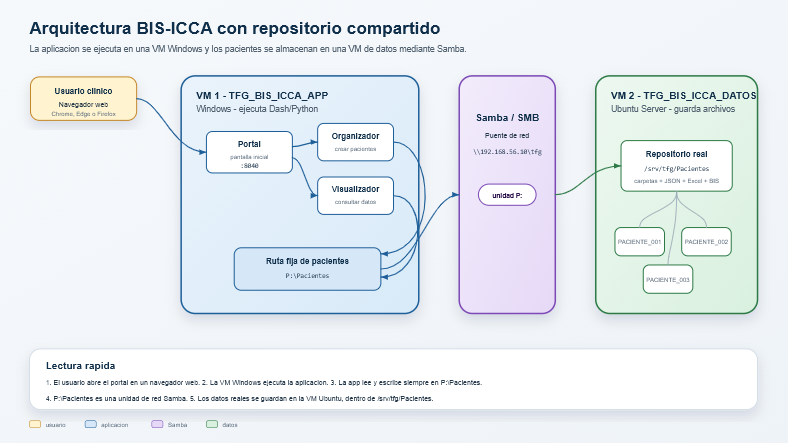
\includegraphics[width=0.9\linewidth,height=\textheight,keepaspectratio]{img/esquema_arquitectura_ubu.png}

}

\caption{\label{fig-diseno-despliegue}Diseño de despliegue mediante
máquinas virtuales. Fuente: elaboración propia, generada con apoyo de
ChatGPT.}

\end{figure}%

La Figura~\ref{fig-diseno-despliegue} muestra la separación entre la
máquina virtual de aplicación y la máquina virtual de datos.

De esta forma, la aplicación trabaja siempre sobre una ruta fija de
pacientes, evitando que el usuario tenga que seleccionar manualmente la
carpeta de trabajo.

\subsection{Organización de los
datos}\label{organizaciuxf3n-de-los-datos}

El sistema no utiliza una base de datos relacional. La información se
organiza mediante carpetas y archivos, manteniendo una estructura común
para todos los pacientes.

\begin{Shaded}
\begin{Highlighting}[]
\NormalTok{Pacientes/}
\NormalTok{├── PACIENTE\_001/}
\NormalTok{│   ├── paciente.json}
\NormalTok{│   ├── ICCA\_ORIGINALES/}
\NormalTok{│   └── SESIONES/}
\NormalTok{│       ├── SESION\_001\_...}
\NormalTok{│       │   ├── sesion.json}
\NormalTok{│       │   ├── BIS/}
\NormalTok{│       │   └── ICCA/}
\NormalTok{│       └── SESION\_002\_...}
\NormalTok{│           ├── sesion.json}
\NormalTok{│           ├── BIS/}
\NormalTok{│           └── ICCA/}
\NormalTok{└── PACIENTE\_002/}
\NormalTok{    └── ...}
\end{Highlighting}
\end{Shaded}

Cada paciente dispone de una carpeta propia, donde se almacenan sus
sesiones BIS, los registros ICCA asociados y los archivos auxiliares
generados por la aplicación.

\subsection{Organización interna del
código}\label{organizaciuxf3n-interna-del-cuxf3digo}

El código se divide en aplicaciones independientes y módulos internos
agrupados por responsabilidad.

El organizador incluye la lógica necesaria para:

\begin{itemize}
\tightlist
\item
  detectar sesiones BIS;
\item
  analizar intervalos temporales;
\item
  asociar registros ICCA;
\item
  crear la estructura de carpetas de cada paciente;
\item
  generar archivos auxiliares.
\end{itemize}

El visualizador incluye la lógica necesaria para:

\begin{itemize}
\tightlist
\item
  leer exportaciones BIS;
\item
  reconstruir o cargar la matriz DSA;
\item
  generar vistas temporales;
\item
  representar la señal BIS, EMG y DSA;
\item
  cargar y visualizar variables clínicas ICCA;
\item
  generar informes PDF.
\end{itemize}

\subsection{Principales módulos del
sistema}\label{principales-muxf3dulos-del-sistema}

\begin{longtable}[]{@{}
  >{\raggedright\arraybackslash}p{(\linewidth - 2\tabcolsep) * \real{0.5000}}
  >{\raggedright\arraybackslash}p{(\linewidth - 2\tabcolsep) * \real{0.5000}}@{}}
\caption{Principales módulos del sistema y responsabilidades
asociadas}\label{tbl-modulos-sistema}\tabularnewline
\toprule\noalign{}
\begin{minipage}[b]{\linewidth}\raggedright
Módulo
\end{minipage} & \begin{minipage}[b]{\linewidth}\raggedright
Responsabilidad
\end{minipage} \\
\midrule\noalign{}
\endfirsthead
\toprule\noalign{}
\begin{minipage}[b]{\linewidth}\raggedright
Módulo
\end{minipage} & \begin{minipage}[b]{\linewidth}\raggedright
Responsabilidad
\end{minipage} \\
\midrule\noalign{}
\endhead
\bottomrule\noalign{}
\endlastfoot
\texttt{pacientes.py} & Creación, edición, eliminación y listado de
pacientes. \\
\texttt{intervalos.py} & Análisis temporal de sesiones BIS y registros
ICCA. \\
\texttt{excel\_icca.py} & Lectura y preparación de archivos ICCA. \\
\texttt{libros.py} & Generación de archivos Excel auxiliares. \\
\texttt{carpeta\_bis.py} & Detección de exportaciones BIS. \\
\texttt{validacion\_bis.py} & Validación de la estructura de una
exportación BIS. \\
\texttt{lectura\_spa.py} & Lectura de variables procesadas de BIS. \\
\texttt{lectura\_fa.py} & Lectura de la matriz DSA original. \\
\texttt{reconstruccion.py} & Reconstrucción de la DSA a partir del EEG
crudo. \\
\texttt{alineacion\_temporal.py} & Alineación temporal y detección de
discontinuidades. \\
\texttt{bandas.py} & Cálculo del ratio alfa-delta. \\
\texttt{vistas\_temporales.py} & División del registro en tramos
temporales. \\
\texttt{figuras.py} & Generación de figuras interactivas. \\
\texttt{figuras\_estaticas.py} & Generación de figuras estáticas para
informes. \\
\texttt{visualizacion\_icca.py} & Preparación y visualización de
variables clínicas ICCA. \\
\texttt{pacientes\_icca.py} & Preparación de sesiones con información
ICCA. \\
\texttt{informe\_pdf.py} & Generación del informe PDF del caso
visualizado. \\
\end{longtable}

\subsection{Justificación del
diseño}\label{justificaciuxf3n-del-diseuxf1o}

El diseño propuesto responde a las necesidades principales del proyecto:
organizar sesiones BIS e información ICCA, permitir su consulta
posterior y facilitar una posible adaptación a un entorno hospitalario.

La separación entre organizador y visualizador evita mezclar tareas de
preparación de datos con tareas de consulta. A su vez, el uso de una
estructura fija de carpetas permite mantener los archivos originales y
auxiliares asociados a cada paciente, sin necesidad de implantar una
base de datos.

Por último, la arquitectura basada en máquinas virtuales permite simular
un escenario de uso en intranet, separando la ejecución de la aplicación
del almacenamiento común de los pacientes.

%% ══════════════════════════════════════════════════════
%%  APÉNDICE C – Especificación de Requisitos
%% ══════════════════════════════════════════════════════

\apendice{Especificación de Requisitos}

\section{Diagrama de casos de uso}\label{diagrama-de-casos-de-uso}

El sistema distingue dos actores principales: el \textbf{usuario
clínico}, que organiza pacientes y consulta sus sesiones, y el
\textbf{administrador}, que gestiona la disponibilidad del repositorio
de pacientes en la máquina virtual compartida (Anexo B). En la práctica,
ambos roles pueden recaer sobre la misma persona, pero se diferencian
porque no todas las acciones requieren privilegios de administración.

\begin{figure}

\centering{

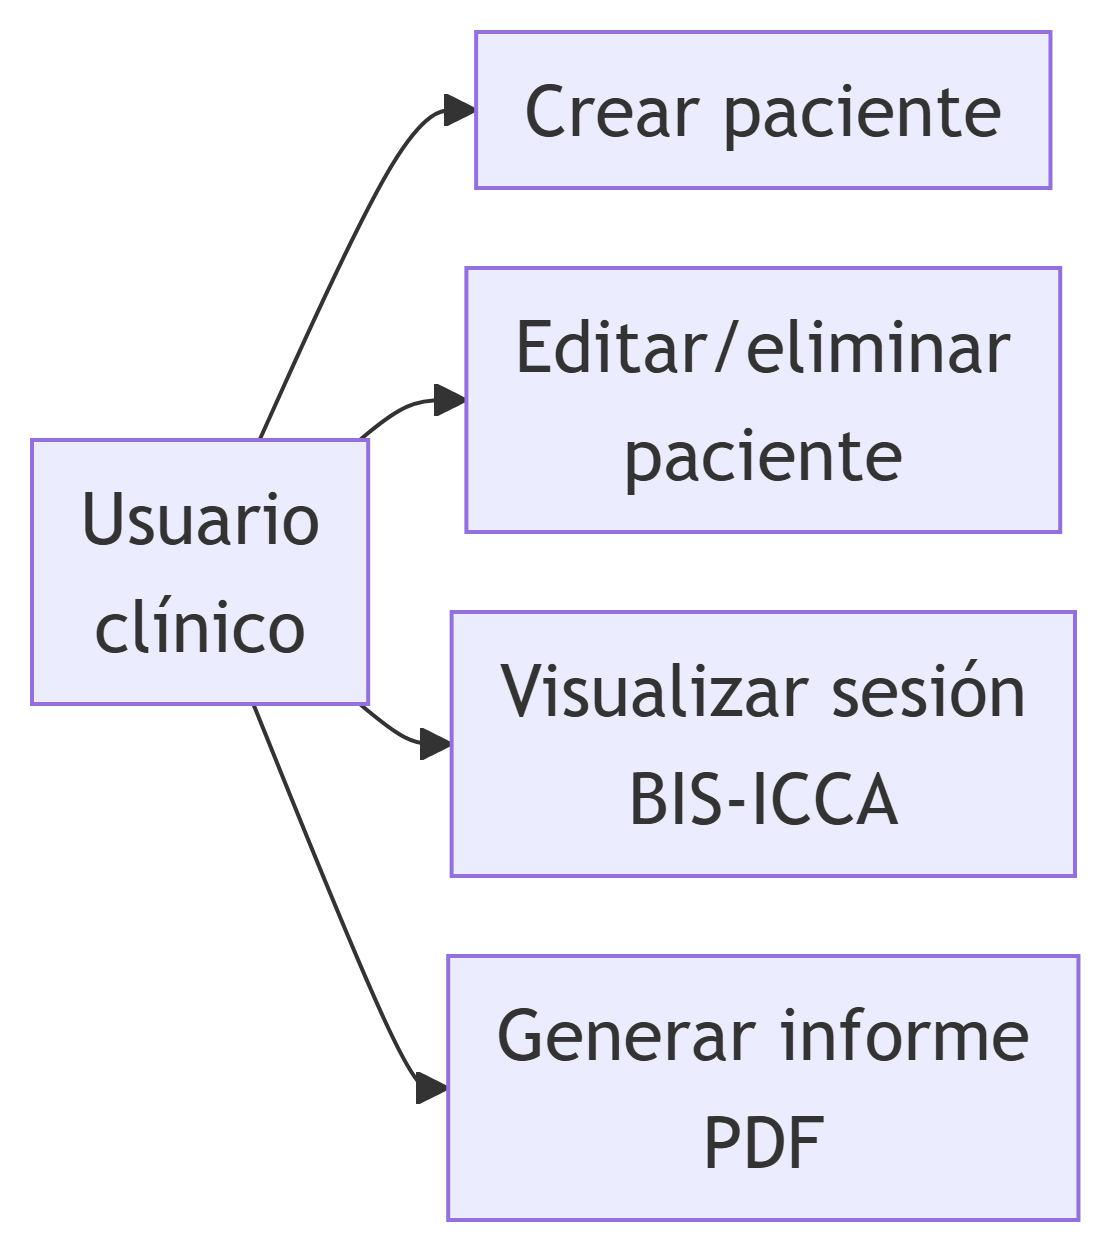
\includegraphics[width=6in,height=6.76in]{anexos_files/figure-latex/mermaid-figure-1.png}

}

\caption{\label{fig-casos-uso}Diagrama de casos de uso principales del
sistema. Fuente: elaboración propia.}

\end{figure}%

\section{Explicación de los casos de
uso}\label{explicaciuxf3n-de-los-casos-de-uso}

A continuación se detallan los cuatro casos de uso principales del
sistema.

\begin{table}[p]
    \centering
    \begin{tabularx}{\linewidth}{ p{0.21\columnwidth} p{0.71\columnwidth} }
        \toprule
        \textbf{CU-1}    & \textbf{Crear paciente}\\
        \toprule
        \textbf{Versión}              & 1.0    \\
        \textbf{Autor}                & Alumna \\
        \textbf{Requisitos asociados} & RF-01, RF-02, RF-03 \\
        \textbf{Descripción}          & El usuario selecciona una o varias sesiones BIS y, opcionalmente, uno o varios archivos ICCA compatibles, y la aplicación crea una nueva carpeta de paciente con las copias organizadas y los manifiestos correspondientes. \\
        \textbf{Precondición}         & Debe seleccionarse al menos una sesión BIS válida (con archivo \texttt{.spa}). \\
        \textbf{Acciones}             &
        \begin{enumerate}
            \def\labelenumi{\arabic{enumi}.}
            \tightlist
            \item El usuario selecciona la carpeta o carpetas de sesión BIS.
            \item El usuario selecciona, si procede, uno o varios archivos ICCA.
            \item La aplicación analiza los intervalos temporales y el solapamiento entre fuentes.
            \item El usuario revisa las asignaciones detectadas.
            \item El usuario confirma la creación del paciente.
        \end{enumerate}\\
        \textbf{Postcondición}        & Se crea la carpeta \texttt{PACIENTE\_NNN} con sus sesiones, manifiestos y, si procede, el Excel ICCA auxiliar de cada sesión. \\
        \textbf{Excepciones}          & Sesiones BIS solapadas en más de 30 s en el mismo paciente; archivo ICCA o sesión BIS ya asignados a otro paciente; ausencia de sesiones BIS seleccionadas. \\
        \textbf{Importancia}          & Alta \\
        \bottomrule
    \end{tabularx}
    \caption{CU-1 Crear paciente.}
\end{table}

\begin{table}[p]
    \centering
    \begin{tabularx}{\linewidth}{ p{0.21\columnwidth} p{0.71\columnwidth} }
        \toprule
        \textbf{CU-2}    & \textbf{Editar/eliminar paciente}\\
        \toprule
        \textbf{Versión}              & 1.0    \\
        \textbf{Autor}                & Alumna \\
        \textbf{Requisitos asociados} & RF-04, RF-05 \\
        \textbf{Descripción}          & El usuario modifica las fuentes asignadas a un paciente ya creado (añadiendo o retirando sesiones BIS y archivos ICCA) o elimina por completo un paciente existente. \\
        \textbf{Precondición}         & Debe existir al menos un paciente ya creado. \\
        \textbf{Acciones}             &
        \begin{enumerate}
            \def\labelenumi{\arabic{enumi}.}
            \tightlist
            \item El usuario selecciona un paciente de la lista de gestión.
            \item El usuario añade o retira sesiones BIS o archivos ICCA.
            \item La aplicación vuelve a validar los intervalos y solapamientos antes de guardar.
            \item El usuario confirma la edición, o bien solicita eliminar el paciente con confirmación expresa.
        \end{enumerate}\\
        \textbf{Postcondición}        & Se actualiza la carpeta del paciente con las nuevas fuentes, o se elimina por completo si así se solicitó. \\
        \textbf{Excepciones}          & Los mismos conflictos de solapamiento y reutilización de fuentes que en CU-1; intento de eliminación sin confirmación. \\
        \textbf{Importancia}          & Media \\
        \bottomrule
    \end{tabularx}
    \caption{CU-2 Editar/eliminar paciente.}
\end{table}

\begin{table}[p]
    \centering
    \begin{tabularx}{\linewidth}{ p{0.21\columnwidth} p{0.71\columnwidth} }
        \toprule
        \textbf{CU-3}    & \textbf{Visualizar sesión BIS-ICCA}\\
        \toprule
        \textbf{Versión}              & 1.0    \\
        \textbf{Autor}                & Alumna \\
        \textbf{Requisitos asociados} & RF-06, RF-07, RF-08 \\
        \textbf{Descripción}          & El usuario selecciona un paciente y una de sus sesiones BIS, y la aplicación carga la DSA (original o reconstruida), las variables procesadas del monitor y, si está disponible, la información clínica ICCA asociada al intervalo. \\
        \textbf{Precondición}         & Debe existir al menos un paciente con una sesión BIS organizada. \\
        \textbf{Acciones}             &
        \begin{enumerate}
            \def\labelenumi{\arabic{enumi}.}
            \tightlist
            \item El usuario selecciona un paciente de la lista.
            \item El usuario selecciona una sesión BIS de ese paciente.
            \item La aplicación detecta si existe un archivo \texttt{.f\_a} válido o si es necesario reconstruir la DSA.
            \item La aplicación representa la DSA, las variables BIS y, si existen, las variables ICCA.
            \item El usuario puede seleccionar un tramo horario y ajustar la duración de la vista.
        \end{enumerate}\\
        \textbf{Postcondición}        & Se muestra la visualización conjunta del intervalo seleccionado. \\
        \textbf{Excepciones}          & Ausencia de archivo \texttt{.f\_a} válido y de señal cruda completa (no es posible reconstruir la DSA); sesión sin información ICCA compatible. \\
        \textbf{Importancia}          & Alta \\
        \bottomrule
    \end{tabularx}
    \caption{CU-3 Visualizar sesión BIS-ICCA.}
\end{table}

\begin{table}[p]
    \centering
    \begin{tabularx}{\linewidth}{ p{0.21\columnwidth} p{0.71\columnwidth} }
        \toprule
        \textbf{CU-4}    & \textbf{Generar informe PDF}\\
        \toprule
        \textbf{Versión}              & 1.0    \\
        \textbf{Autor}                & Alumna \\
        \textbf{Requisitos asociados} & RF-09 \\
        \textbf{Descripción}          & A partir de una sesión ya cargada en el visualizador, el usuario genera un documento PDF con una portada identificativa, la representación de la DSA y un resumen de la información clínica ICCA del intervalo mostrado. \\
        \textbf{Precondición}         & Debe haberse cargado previamente una sesión en el visualizador (CU-3). \\
        \textbf{Acciones}             &
        \begin{enumerate}
            \def\labelenumi{\arabic{enumi}.}
            \tightlist
            \item El usuario solicita la generación del informe desde la sesión visualizada.
            \item La aplicación construye la portada con los datos identificativos y el intervalo mostrado.
            \item La aplicación genera la página de la DSA y el resumen ICCA.
            \item El usuario descarga el archivo PDF resultante.
        \end{enumerate}\\
        \textbf{Postcondición}        & Se genera un archivo PDF descargable asociado a la sesión y al intervalo mostrados. \\
        \textbf{Excepciones}          & Ausencia de información ICCA (el informe se genera igualmente, indicando que no hay datos clínicos disponibles). \\
        \textbf{Importancia}          & Media \\
        \bottomrule
    \end{tabularx}
    \caption{CU-4 Generar informe PDF.}
\end{table}

\section{Prototipos de interfaz o interacción con el
proyecto}\label{prototipos-de-interfaz-o-interacciuxf3n-con-el-proyecto}

A continuación se muestran las pantallas más representativas de cada
caso de uso. Las capturas correspondientes al resultado final del
visualizador (DSA, variables BIS e ICCA) y al informe PDF generado
(CU-4) ya se muestran con su contexto de resultado en el capítulo de
Resultados de la memoria, por lo que aquí no se duplican.

\subsection{CU-1: Crear paciente}\label{cu-1-crear-paciente}

La creación de un paciente parte de la pantalla inicial del organizador
(Figura~\ref{fig-inicio-organizador}), donde el usuario aporta las
sesiones BIS y los archivos ICCA. Antes de confirmar, la aplicación
muestra una revisión de las asignaciones detectadas
(Figura~\ref{fig-revision-paciente}), incluyendo el solapamiento
calculado entre cada sesión BIS y las plantillas ICCA compatibles.

\begin{figure}

\centering{

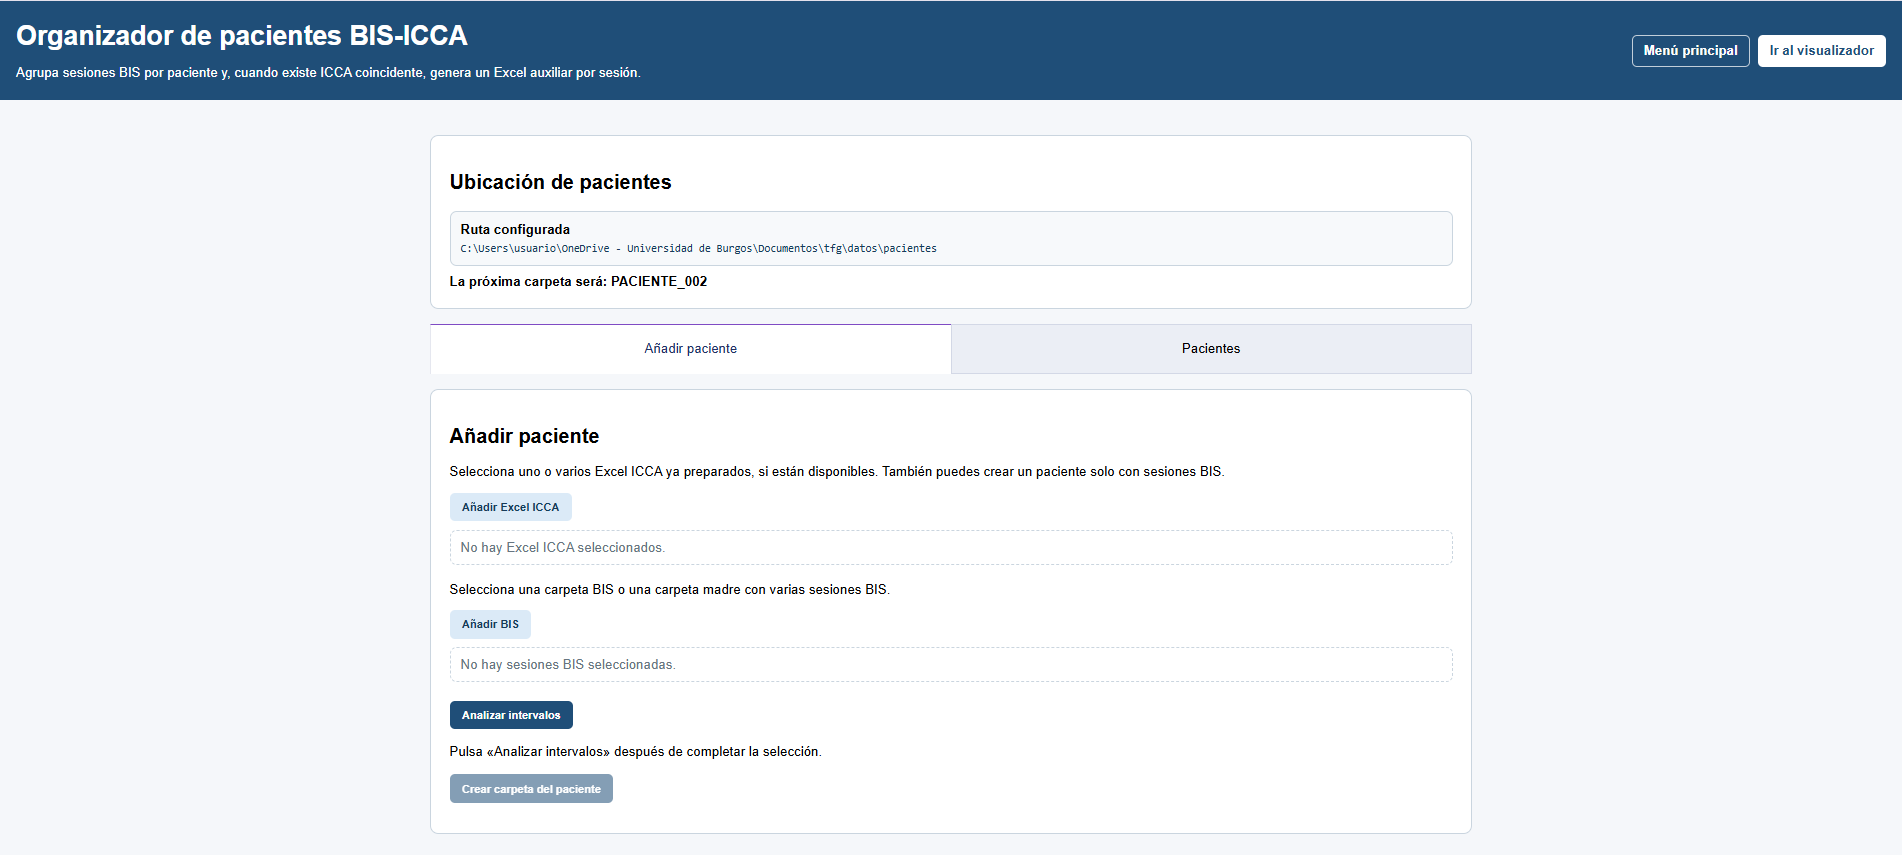
\includegraphics[width=0.9\linewidth,height=\textheight,keepaspectratio]{img/capturas_app_organizador/cap_inicio_organizador.png}

}

\caption{\label{fig-inicio-organizador}Pantalla inicial de la aplicación
de organización de datos. Fuente: elaboración propia.}

\end{figure}%

\begin{figure}

\centering{

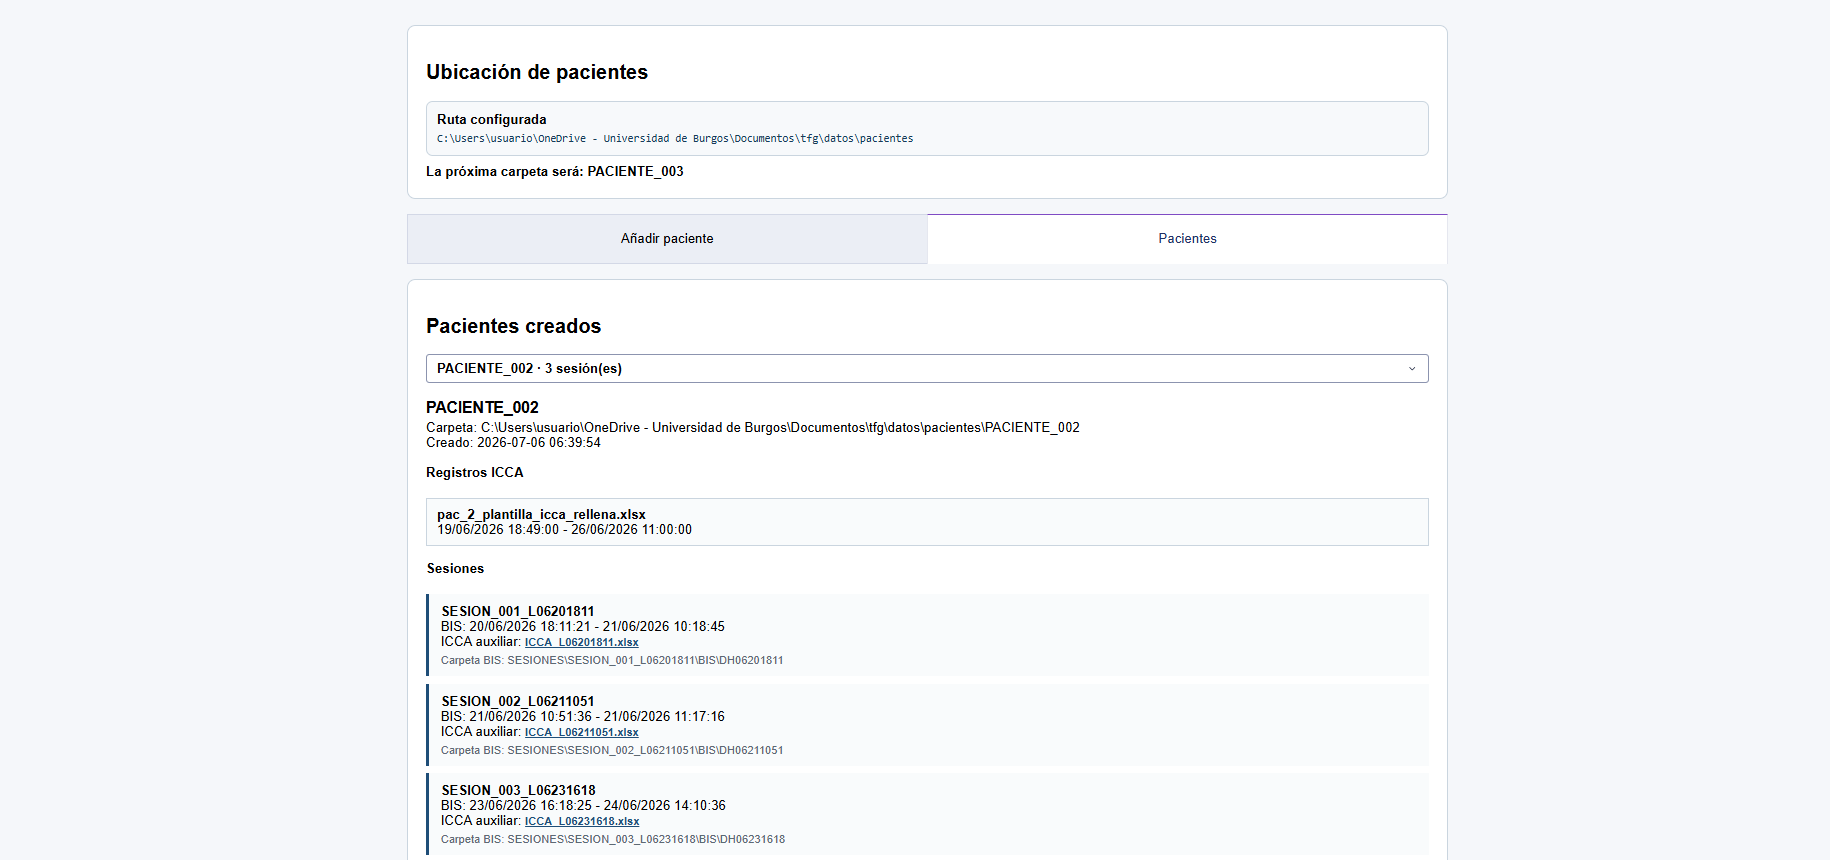
\includegraphics[width=0.9\linewidth,height=\textheight,keepaspectratio]{img/capturas_app_organizador/cap_revision_paciente.png}

}

\caption{\label{fig-revision-paciente}Revisión de las asignaciones antes
de crear el paciente. Fuente: elaboración propia.}

\end{figure}%

Una vez confirmada la creación, el contenido generado para el paciente
(carpetas de sesión, manifiestos y Excel ICCA auxiliar) queda organizado
tal como se muestra en la Figura~\ref{fig-contenido-paciente}.

\begin{figure}

\centering{

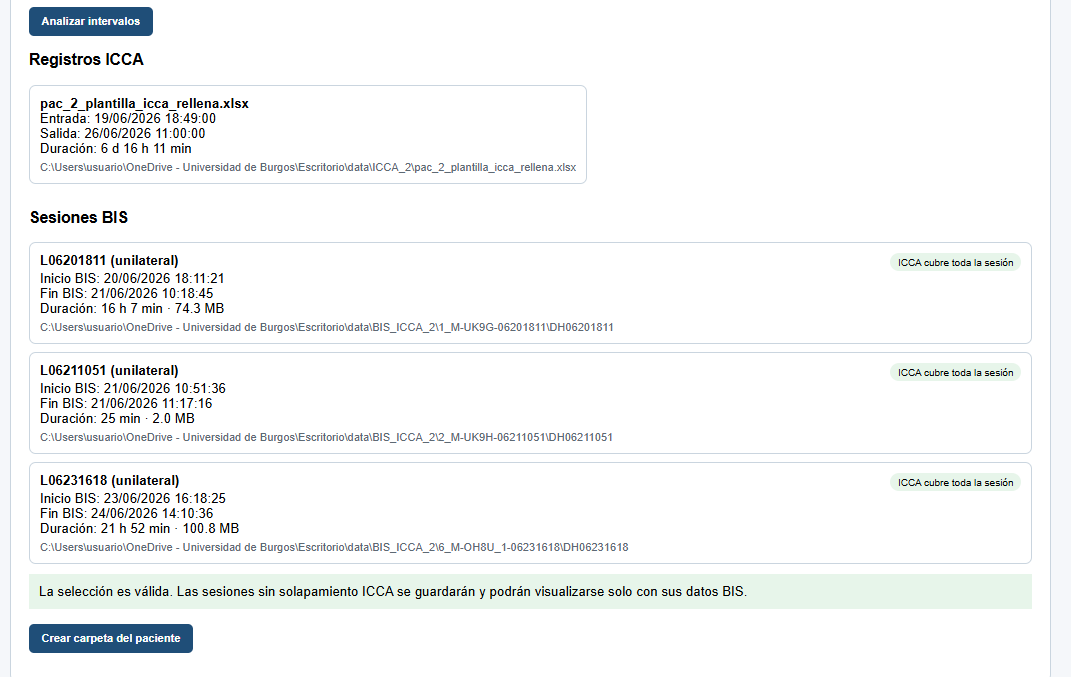
\includegraphics[width=0.9\linewidth,height=\textheight,keepaspectratio]{img/capturas_app_organizador/cap_analisis_contenido_sesion.png}

}

\caption{\label{fig-contenido-paciente}Contenido generado para una
sesión organizada por paciente, con la exportación BIS y el Excel ICCA
auxiliar. Fuente: elaboración propia.}

\end{figure}%

\subsection{CU-2: Editar/eliminar
paciente}\label{cu-2-editareliminar-paciente}

La edición de un paciente ya creado permite añadir o retirar sesiones
BIS y archivos ICCA sin modificar los originales, tal y como se muestra
en la Figura~\ref{fig-editar-paciente}.

\begin{figure}

\centering{

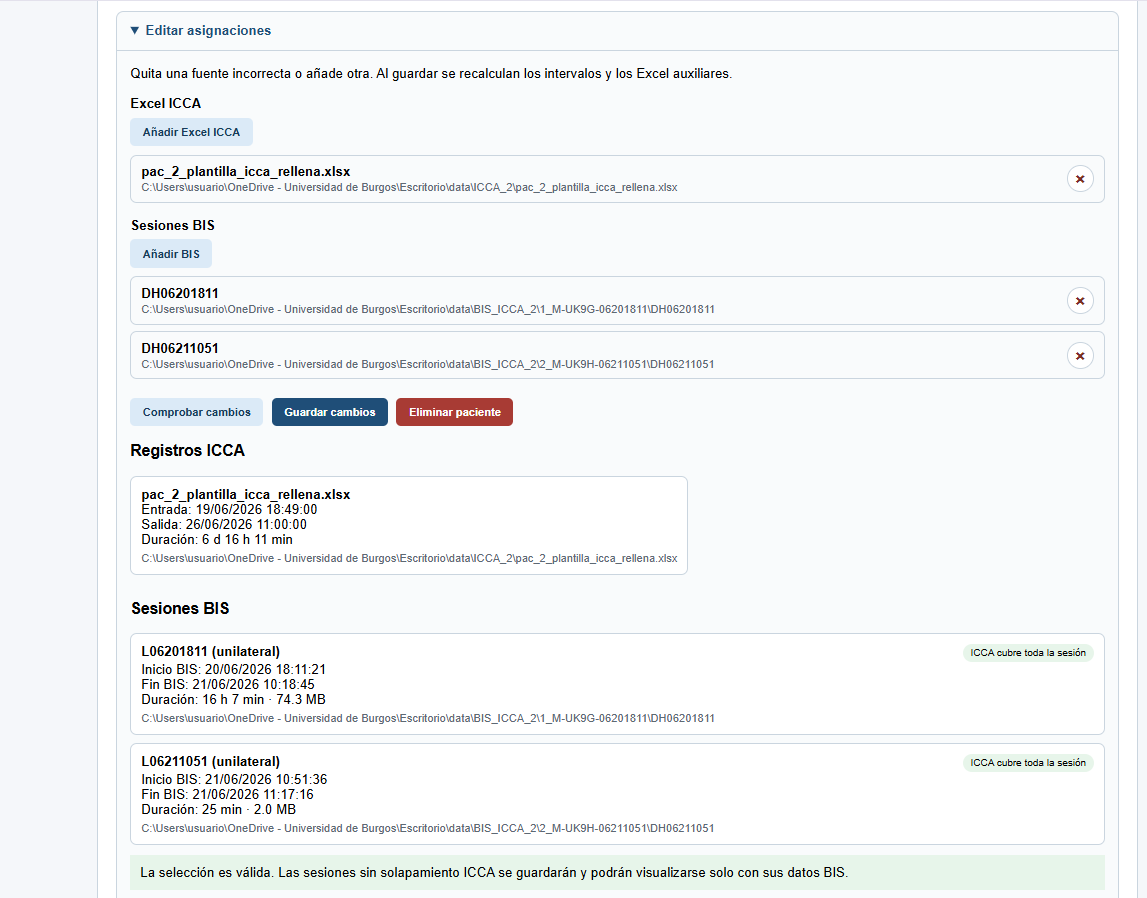
\includegraphics[width=0.9\linewidth,height=\textheight,keepaspectratio]{img/capturas_app_organizador/cap_editar_paciente.png}

}

\caption{\label{fig-editar-paciente}Edición de asignaciones de un
paciente ya creado. Fuente: elaboración propia.}

\end{figure}%

\subsection{CU-3: Visualizar sesión
BIS-ICCA}\label{cu-3-visualizar-sesiuxf3n-bis-icca}

El visualizador parte de una pantalla inicial
(Figura~\ref{fig-visualizador-inicio}) desde la que se accede a la
selección de paciente y sesión
(Figura~\ref{fig-visualizador-seleccion}).

\begin{figure}

\centering{

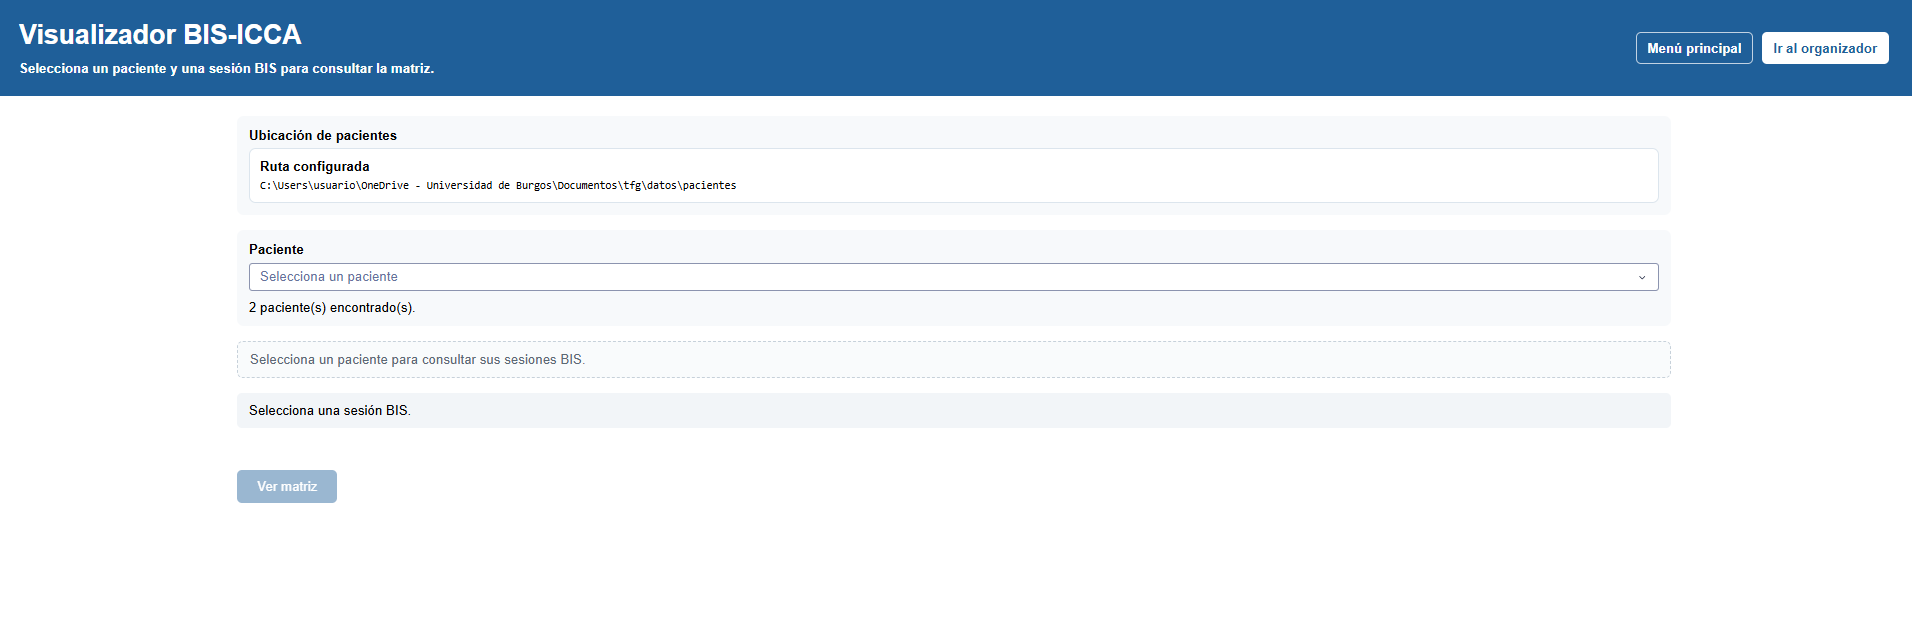
\includegraphics[width=0.9\linewidth,height=\textheight,keepaspectratio]{img/capturas_app_visualizador/visual_inicio.png}

}

\caption{\label{fig-visualizador-inicio}Pantalla inicial del
visualizador. Fuente: elaboración propia.}

\end{figure}%

\begin{figure}

\centering{

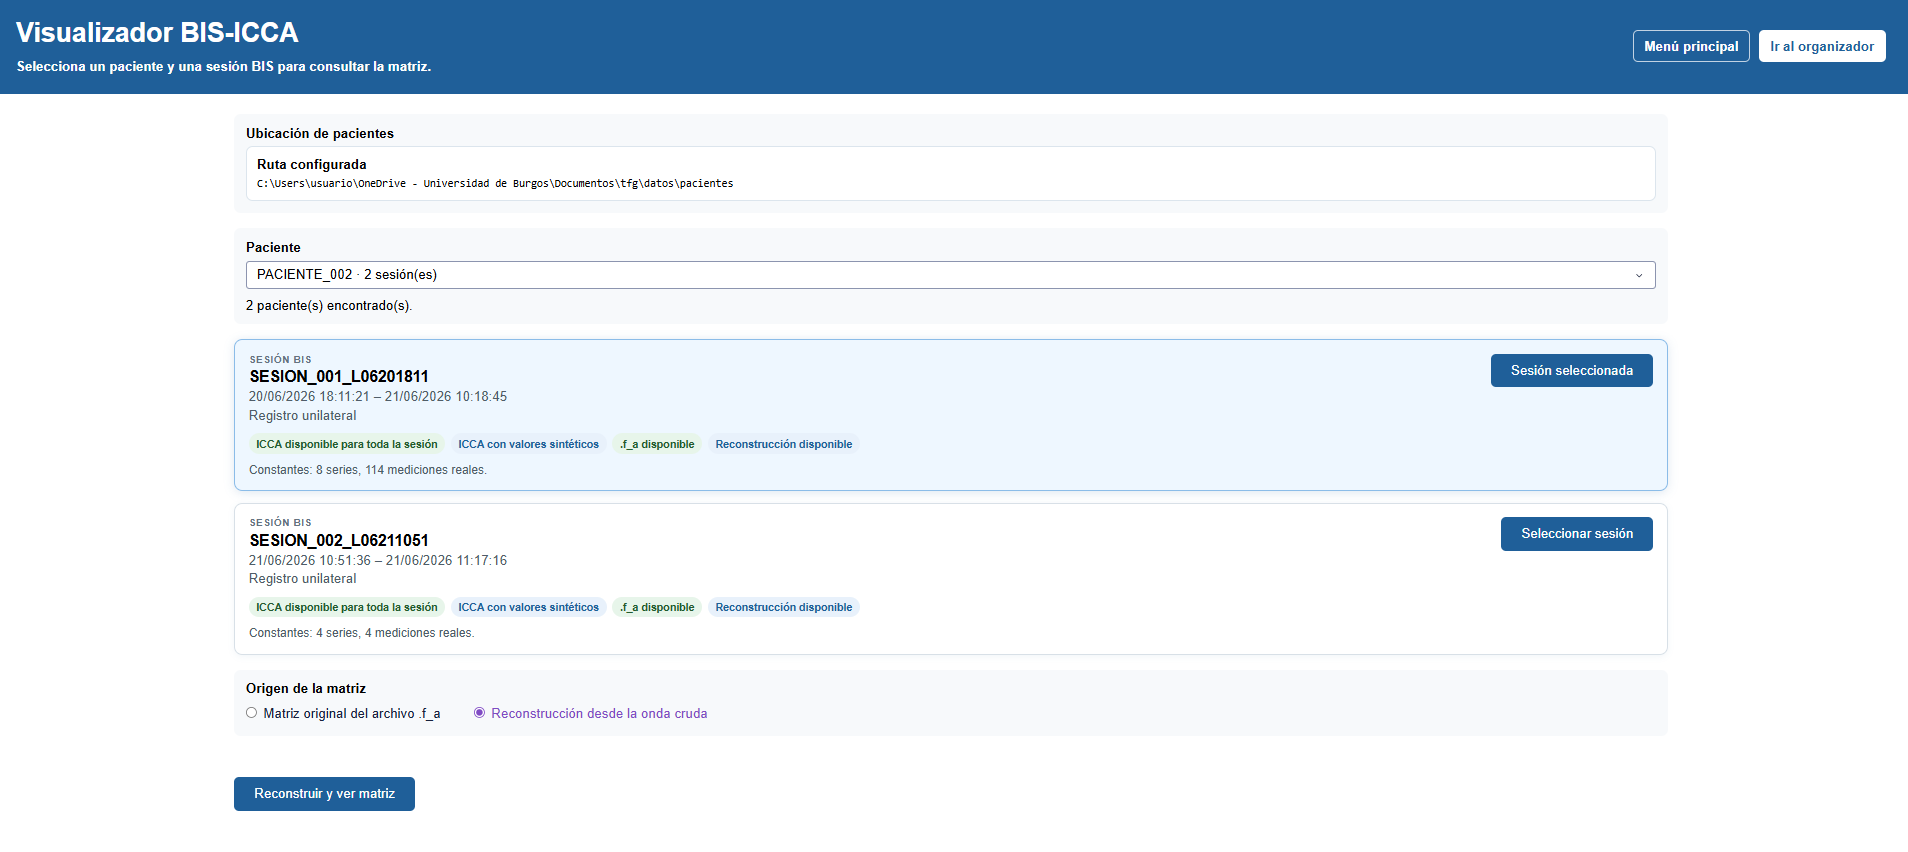
\includegraphics[width=0.9\linewidth,height=\textheight,keepaspectratio]{img/capturas_app_visualizador/visual_paciente_seleccionado.png}

}

\caption{\label{fig-visualizador-seleccion}Selección de paciente y
sesión BIS en el visualizador. Fuente: elaboración propia.}

\end{figure}%

El resultado de la carga (DSA, variables BIS e información ICCA) se
muestra con su contexto de resultado en el capítulo de Resultados de la
memoria.

\subsection{CU-4: Generar informe PDF}\label{cu-4-generar-informe-pdf}

El resultado de este caso de uso, el propio informe PDF generado, se
muestra en el capítulo de Resultados de la memoria.

%% ══════════════════════════════════════════════════════
%%  APÉNDICE D – Manual de Usuario
%% ══════════════════════════════════════════════════════

\apendice{Documentación de usuario}

\section{Requisitos software y hardware para ejecutar el
proyecto}\label{requisitos-software-y-hardware-para-ejecutar-el-proyecto}

Para utilizar la aplicación BIS-ICCA es necesario disponer de un equipo
con sistema operativo Windows y un navegador web moderno. La aplicación
se ha desarrollado en Python utilizando Dash, por lo que su ejecución se
realiza desde un entorno Python previamente configurado.

Los requisitos mínimos recomendados son:

\begin{itemize}
\tightlist
\item
  Sistema operativo: Windows 10 o superior.
\item
  Memoria RAM: al menos 8 GB, recomendable 16 GB si se trabaja con
  sesiones BIS largas.
\item
  Procesador: de 64 bits.
\item
  Navegador web: Google Chrome, Microsoft Edge o Mozilla Firefox.
\item
  Python: versión 3.12 o compatible.
\item
  Espacio en disco suficiente para almacenar las sesiones BIS, los
  registros ICCA y los informes generados.
\end{itemize}

No es necesario instalar una base de datos externa, ya que el sistema
organiza la información mediante una estructura de carpetas y archivos
(Anexo B). Cada paciente dispone de su propia carpeta, donde se guardan
las sesiones BIS, los registros ICCA asociados y los archivos auxiliares
generados por la aplicación.

Para la simulación del entorno hospitalario se emplean máquinas
virtuales: una para ejecutar la aplicación y otra para almacenar los
datos de pacientes mediante una carpeta compartida por red (ver diseño
de despliegue en el Anexo B).

\section{Instalación y puesta en
marcha}\label{instalaciuxf3n-y-puesta-en-marcha}

La aplicación puede ejecutarse en dos escenarios: en local durante el
desarrollo, y en un entorno virtualizado para simular su funcionamiento
dentro de una intranet hospitalaria.

\subsection{Ejecución local}\label{ejecuciuxf3n-local}

Para ejecutar la aplicación en local, se debe abrir una terminal de
PowerShell y situarse en la carpeta del proyecto:

\begin{Shaded}
\begin{Highlighting}[]
\FunctionTok{cd} \StringTok{"C:\textbackslash{}Users\textbackslash{}usuario\textbackslash{}OneDrive {-} Universidad de Burgos\textbackslash{}Documentos\textbackslash{}tfg\textbackslash{}aplicaciones"}
\end{Highlighting}
\end{Shaded}

A continuación, se lanza el script de inicio:

\begin{Shaded}
\begin{Highlighting}[]
\OperatorTok{.}\NormalTok{\textbackslash{}iniciar\_aplicaciones}\OperatorTok{.}\FunctionTok{ps1} \OperatorTok{{-}}\NormalTok{PacientesDir }\StringTok{"..\textbackslash{}datos\textbackslash{}pacientes"} \OperatorTok{{-}}\NormalTok{RutaPacientesFija}
\end{Highlighting}
\end{Shaded}

Una vez iniciado el sistema, se accede desde el navegador a la siguiente
dirección:

\begin{Shaded}
\begin{Highlighting}[]
\NormalTok{http://127.0.0.1:8040}
\end{Highlighting}
\end{Shaded}

Esta dirección abre el portal principal de la aplicación, desde el que
se puede acceder al organizador de pacientes o al visualizador. El
proceso de instalación del entorno (creación del entorno virtual e
instalación de dependencias) se detalla en el Anexo E.

\subsection{Ejecución en entorno con máquinas
virtuales}\label{ejecuciuxf3n-en-entorno-con-muxe1quinas-virtuales}

Para simular el funcionamiento en un entorno hospitalario, se plantea
una arquitectura con dos máquinas virtuales:

\begin{itemize}
\tightlist
\item
  Una \textbf{máquina virtual de aplicación}, donde se ejecuta el
  sistema BIS-ICCA.
\item
  Una \textbf{máquina virtual de datos}, donde se almacenan los
  pacientes en una ubicación común.
\end{itemize}

La máquina de datos comparte la carpeta de pacientes mediante Samba/SMB.
Desde la máquina de aplicación, esta carpeta se monta como una unidad de
red, por ejemplo:

\begin{Shaded}
\begin{Highlighting}[]
\NormalTok{P:\textbackslash{}Pacientes}
\end{Highlighting}
\end{Shaded}

De esta forma, la aplicación trabaja siempre sobre una ruta fija y el
usuario no tiene que seleccionar manualmente dónde guardar o buscar los
pacientes.

\section{Manuales y demostraciones
prácticas}\label{manuales-y-demostraciones-pruxe1cticas}

\subsection{Acceso al portal
principal}\label{acceso-al-portal-principal}

Al abrir la aplicación desde el navegador, aparece el portal principal
(Figura~\ref{fig-manual-portal}). Desde esta pantalla se puede elegir
entre dos opciones:

\begin{itemize}
\tightlist
\item
  Añadir / gestionar pacientes.
\item
  Visualizar paciente.
\end{itemize}

\begin{figure}

\centering{

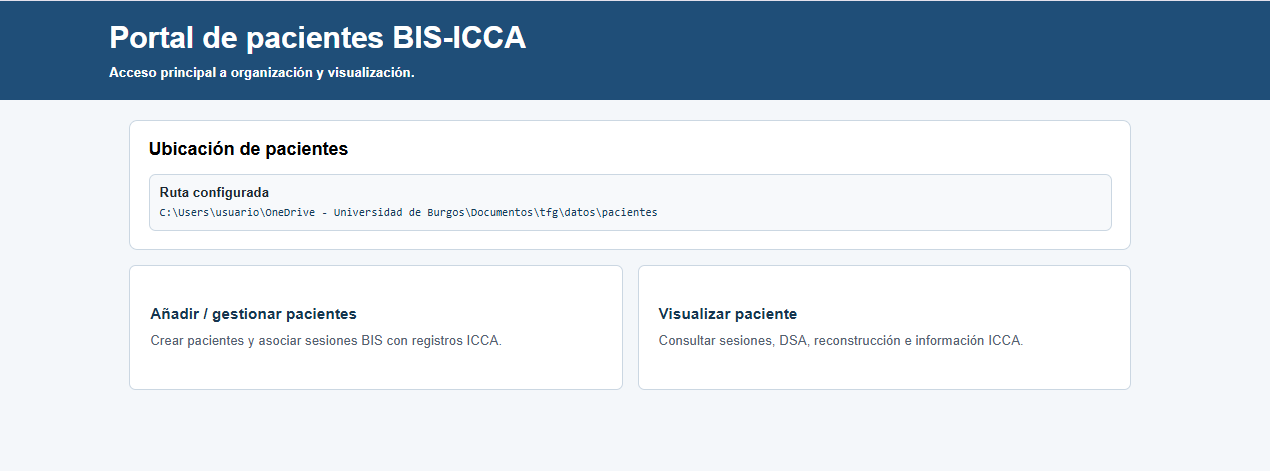
\includegraphics[width=0.9\linewidth,height=\textheight,keepaspectratio]{img/capturas_portal/captura_menu_portal.png}

}

\caption{\label{fig-manual-portal}Portal principal de acceso al sistema.
Fuente: elaboración propia.}

\end{figure}%

El portal funciona como punto de entrada común y permite separar
claramente las tareas de organización de pacientes de las tareas de
consulta o visualización.

\subsection{Añadir o gestionar
pacientes}\label{auxf1adir-o-gestionar-pacientes}

La opción de añadir o gestionar pacientes permite crear nuevos pacientes
a partir de registros ICCA y sesiones BIS. El flujo general es el
siguiente:

\begin{enumerate}
\def\labelenumi{\arabic{enumi}.}
\tightlist
\item
  Seleccionar uno o varios archivos Excel ICCA, si están disponibles.
\item
  Seleccionar una carpeta BIS o una carpeta madre que contenga varias
  sesiones BIS.
\item
  Analizar los intervalos temporales.
\item
  Comprobar que las sesiones se asignan correctamente.
\item
  Crear la carpeta del paciente.
\end{enumerate}

Las capturas de las pantallas correspondientes a este flujo (pantalla
inicial del organizador, revisión de asignaciones y edición de un
paciente ya creado) se muestran en el Anexo C, apartado de prototipos de
interfaz (Figura~\ref{fig-inicio-organizador},
Figura~\ref{fig-revision-paciente} y Figura~\ref{fig-editar-paciente}).

La aplicación genera una estructura de carpetas organizada, en la que se
almacenan las sesiones BIS, los registros ICCA originales y los archivos
auxiliares necesarios para la visualización posterior
(Figura~\ref{fig-contenido-paciente}, Anexo C).

\subsection{Visualizar paciente}\label{visualizar-paciente}

La opción de visualizar paciente permite consultar los pacientes ya
creados. El flujo general es el siguiente:

\begin{enumerate}
\def\labelenumi{\arabic{enumi}.}
\tightlist
\item
  Seleccionar un paciente de la lista.
\item
  Seleccionar una sesión BIS asociada.
\item
  Elegir el tramo temporal que se desea visualizar.
\item
  Consultar la matriz DSA, el índice BIS, la señal EMG y la información
  clínica ICCA disponible.
\item
  Exportar un informe en PDF si se desea conservar o imprimir la
  visualización del caso.
\end{enumerate}

Las capturas de la pantalla inicial del visualizador y de la selección
de paciente y sesión se muestran en el Anexo C
(Figura~\ref{fig-visualizador-inicio} y
Figura~\ref{fig-visualizador-seleccion}). El resultado de la carga (DSA,
variables BIS e información ICCA) se muestra en el capítulo de
Resultados de la memoria.

\subsection{Exportación de informe
PDF}\label{exportaciuxf3n-de-informe-pdf}

El visualizador permite generar un informe PDF del intervalo
seleccionado. Este informe incluye una portada con los datos
identificativos de la sesión, la representación de la DSA junto con las
variables procesadas del monitor, y un resumen de la información clínica
ICCA disponible para ese intervalo (constantes vitales, análisis
clínicos y perfusiones). El resultado de este proceso se muestra en el
capítulo de Resultados de la memoria.

El informe está pensado como documento auxiliar para revisión o
impresión, pero no sustituye la valoración clínica ni la revisión de los
registros originales.

\section{Consideraciones de uso}\label{consideraciones-de-uso}

Todos los usuarios acceden a la misma ubicación común de pacientes. La
aplicación no distingue entre usuarios individuales ni incorpora roles
de administrador, ya que el objetivo es que los pacientes creados puedan
ser consultados por cualquier profesional autorizado dentro del entorno
de trabajo.

Se recomienda no modificar manualmente la estructura interna de las
carpetas de pacientes, salvo para realizar copias de seguridad o
trasladar el repositorio completo.

%% ══════════════════════════════════════════════════════
%%  APÉNDICE E – Manual del Desarrollador
%% ══════════════════════════════════════════════════════

\apendice{Manual del desarrollador e investigador}

\section{Estructura de directorios}\label{estructura-de-directorios}

El proyecto se organiza en torno a una carpeta principal que contiene
las aplicaciones desarrolladas, los datos de trabajo y los archivos
auxiliares necesarios para la ejecución local del sistema. La estructura
general es la siguiente:

\begin{Shaded}
\begin{Highlighting}[]
\NormalTok{tfg/}
\NormalTok{├── aplicaciones/}
\NormalTok{│   ├── portal\_bis\_icca/}
\NormalTok{│   ├── organizador\_bis\_icca/}
\NormalTok{│   │   └── requirements.txt}
\NormalTok{│   ├── visualizador\_bis\_icca/}
\NormalTok{│   │   └── requirements.txt}
\NormalTok{│   ├── requirements.txt}
\NormalTok{│   ├── preparar\_entorno.ps1}
\NormalTok{│   ├── iniciar\_aplicaciones.ps1}
\NormalTok{│   └── detener\_aplicaciones.ps1}
\NormalTok{├── datos/}
\NormalTok{│   └── pacientes/}
\NormalTok{├── README.md}
\NormalTok{└── .gitignore}
\end{Highlighting}
\end{Shaded}

La carpeta \texttt{aplicaciones/} contiene el sistema ejecutable del
proyecto, dividido en tres aplicaciones complementarias:

\begin{itemize}
\tightlist
\item
  \texttt{portal\_bis\_icca/}: pantalla inicial de acceso al sistema.
\item
  \texttt{organizador\_bis\_icca/}: aplicación encargada de organizar
  pacientes, asociar sesiones BIS y archivos ICCA, y generar la
  estructura de carpetas de trabajo.
\item
  \texttt{visualizador\_bis\_icca/}: aplicación principal de
  visualización conjunta de DSA, parámetros BIS y variables clínicas
  ICCA.
\end{itemize}

La versión final del proyecto centraliza las tres aplicaciones dentro de
la carpeta \texttt{aplicaciones/}. Cualquier referencia previa a rutas
directas como \texttt{tfg/organizador\_bis\_icca/} corresponde a una
estructura anterior del desarrollo, ya sustituida por
\texttt{tfg/aplicaciones/organizador\_bis\_icca/}.

Cada aplicación contiene un archivo \texttt{app.py}, que define la
interfaz Dash y sus \emph{callbacks} principales. Las funciones
auxiliares se agrupan en la carpeta \texttt{src/} de cada aplicación,
mientras que las pruebas automáticas se almacenan en su carpeta
\texttt{tests/}.

La carpeta \texttt{datos/pacientes/} contiene las carpetas generadas
para cada paciente durante el uso del sistema, con las sesiones BIS
seleccionadas, los archivos ICCA asociados y los archivos auxiliares
generados para la visualización. Los archivos originales no se modifican
durante este proceso; cuando es necesario, se trabaja sobre copias o
archivos derivados.

Los directorios como \texttt{.venv/}, \texttt{.runtime/},
\texttt{outputs/}, \texttt{tmp/} o carpetas de pruebas temporales no
forman parte del código fuente principal y no deben considerarse
elementos necesarios para la entrega final.

\section{Compilación, instalación y ejecución del
proyecto}\label{compilaciuxf3n-instalaciuxf3n-y-ejecuciuxf3n-del-proyecto}

El proyecto está desarrollado en Python y utiliza Dash para la
construcción de las interfaces web. No requiere compilación en sentido
estricto, pero sí la preparación de un entorno de ejecución con las
dependencias necesarias.

La primera vez que se utilice el sistema, debe abrirse una terminal de
PowerShell en la carpeta de aplicaciones:

\begin{Shaded}
\begin{Highlighting}[]
\FunctionTok{cd} \StringTok{"C:\textbackslash{}Users\textbackslash{}usuario\textbackslash{}OneDrive {-} Universidad de Burgos\textbackslash{}Documentos\textbackslash{}tfg\textbackslash{}aplicaciones"}
\end{Highlighting}
\end{Shaded}

A continuación, se prepara el entorno local:

\begin{Shaded}
\begin{Highlighting}[]
\OperatorTok{.}\NormalTok{\textbackslash{}preparar\_entorno}\OperatorTok{.}\FunctionTok{ps1}
\end{Highlighting}
\end{Shaded}

Este script crea un entorno virtual de Python en
\texttt{aplicaciones/.venv/} e instala las dependencias indicadas en
\texttt{aplicaciones/requirements.txt}.

La carpeta \texttt{aplicaciones/} contiene un archivo
\texttt{requirements.txt} general, utilizado para preparar el entorno
común de ejecución de las tres aplicaciones. Además, el organizador y el
visualizador conservan cada uno su propio \texttt{requirements.txt}, que
documenta las dependencias específicas de esa aplicación y permite su
ejecución independiente si fuera necesario.

Para iniciar las tres aplicaciones se ejecuta:

\begin{Shaded}
\begin{Highlighting}[]
\OperatorTok{.}\NormalTok{\textbackslash{}iniciar\_aplicaciones}\OperatorTok{.}\FunctionTok{ps1} \OperatorTok{{-}}\NormalTok{PacientesDir }\StringTok{"..\textbackslash{}datos\textbackslash{}pacientes"} \OperatorTok{{-}}\NormalTok{RutaPacientesFija}
\end{Highlighting}
\end{Shaded}

Una vez iniciado el sistema, las aplicaciones quedan disponibles en las
siguientes direcciones locales:

\begin{itemize}
\tightlist
\item
  Portal: \url{http://127.0.0.1:8040/}
\item
  Visualizador: \url{http://127.0.0.1:8050/}
\item
  Organizador: \url{http://127.0.0.1:8060/}
\end{itemize}

Para detener las aplicaciones se utiliza:

\begin{Shaded}
\begin{Highlighting}[]
\OperatorTok{.}\NormalTok{\textbackslash{}detener\_aplicaciones}\OperatorTok{.}\FunctionTok{ps1}
\end{Highlighting}
\end{Shaded}

En un despliegue hospitalario, la ruta local \texttt{datos/pacientes}
puede sustituirse por una ruta compartida definida por el servicio
técnico, manteniendo el mismo código de la aplicación.

\section{Pruebas del sistema}\label{pruebas-del-sistema}

Durante el desarrollo se incluyeron pruebas automáticas para comprobar
partes críticas del sistema. Estas pruebas se centran en la lectura y
validación de archivos BIS, la alineación temporal, la reconstrucción de
la DSA, el cálculo de bandas espectrales, la integración de datos ICCA y
la generación de informes.

Las pruebas del visualizador se encuentran en
\texttt{aplicaciones/visualizador\_bis\_icca/tests/}, y las del
organizador en \texttt{aplicaciones/organizador\_bis\_icca/tests/}.

Para ejecutar las pruebas del visualizador puede utilizarse:

\begin{Shaded}
\begin{Highlighting}[]
\FunctionTok{cd} \StringTok{"C:\textbackslash{}Users\textbackslash{}usuario\textbackslash{}OneDrive {-} Universidad de Burgos\textbackslash{}Documentos\textbackslash{}tfg\textbackslash{}aplicaciones\textbackslash{}visualizador\_bis\_icca"}
\OperatorTok{..}\NormalTok{\textbackslash{}}\OperatorTok{.}\FunctionTok{venv}\NormalTok{\textbackslash{}Scripts\textbackslash{}python}\OperatorTok{.}\FunctionTok{exe} \OperatorTok{{-}}\NormalTok{m unittest}
\end{Highlighting}
\end{Shaded}

En caso de ejecutar los tests desde el entorno común de aplicaciones,
debe emplearse el intérprete del entorno virtual creado en
\texttt{aplicaciones/.venv/}.

Además de las pruebas automáticas, se realizaron pruebas funcionales
manuales con registros BIS unilaterales y bilaterales. Estas pruebas
permitieron comprobar la detección de sesiones, la disponibilidad de
matriz original o reconstruida, la visualización por intervalos
temporales, la integración de variables ICCA y la exportación de
informes en PDF.

\section{Instrucciones para la modificación o mejora del
proyecto}\label{instrucciones-para-la-modificaciuxf3n-o-mejora-del-proyecto}

Para ampliar el sistema se recomienda mantener la separación entre
organización de datos, procesamiento BIS, procesamiento ICCA y
visualización. Esta separación facilita modificar una parte del sistema
sin alterar el resto.

\begin{longtable}[]{@{}
  >{\raggedright\arraybackslash}p{(\linewidth - 2\tabcolsep) * \real{0.5000}}
  >{\raggedright\arraybackslash}p{(\linewidth - 2\tabcolsep) * \real{0.5000}}@{}}
\caption{Ubicación de las modificaciones más
habituales}\label{tbl-modificaciones-desarrollador}\tabularnewline
\toprule\noalign{}
\begin{minipage}[b]{\linewidth}\raggedright
Área de modificación
\end{minipage} & \begin{minipage}[b]{\linewidth}\raggedright
Archivos principales
\end{minipage} \\
\midrule\noalign{}
\endfirsthead
\toprule\noalign{}
\begin{minipage}[b]{\linewidth}\raggedright
Área de modificación
\end{minipage} & \begin{minipage}[b]{\linewidth}\raggedright
Archivos principales
\end{minipage} \\
\midrule\noalign{}
\endhead
\bottomrule\noalign{}
\endlastfoot
Reconstrucción de la DSA &
\texttt{visualizador\_bis\_icca/src/reconstruccion.py},
\texttt{alineacion\_temporal.py}, \texttt{figuras.py} \\
Variables clínicas ICCA &
\texttt{visualizador\_bis\_icca/src/visualizacion\_icca.py},
\texttt{pacientes\_icca.py} \\
Organización de pacientes & \texttt{organizador\_bis\_icca/src/} \\
\end{longtable}

Se recomienda no modificar directamente los datos originales exportados
del monitor BIS ni los archivos ICCA originales. Cualquier procesamiento
adicional debe generar archivos auxiliares identificables dentro de la
carpeta del paciente o de la sesión correspondiente.

Como líneas futuras de mejora orientadas al desarrollador, se plantean:

\begin{itemize}
\tightlist
\item
  Incorporar nuevos tipos de variables ICCA cuando estén disponibles.
\item
  Mejorar la validación automática de solapamientos temporales entre
  sesiones BIS e ICCA.
\item
  Añadir nuevos criterios de calidad de señal o artefactos.
\item
  Optimizar la carga de registros de larga duración.
\item
  Ampliar la exportación de informes con nuevas gráficas o resúmenes
  clínicos.
\item
  Preparar una versión desplegable en red hospitalaria con rutas
  compartidas y control de permisos.
\end{itemize}

%% ══════════════════════════════════════════════════════
%%  APÉNDICE F – Descripción de datos
%% ══════════════════════════════════════════════════════

\apendice{Descripción de adquisición y tratamiento de datos}

\section{Introducción}\label{introducciuxf3n-1}

Este apéndice describe los datos empleados en el proyecto, su
procedencia, estructura y tratamiento. El núcleo del trabajo está
formado por las exportaciones generadas por los monitores BIS VISTA y
BIS Advance, junto con las plantillas Excel de variables clínicas
procedentes de ICCA. Las exportaciones BIS incluyen la señal
electroencefalográfica (EEG) cruda, la matriz espectral calculada por el
equipo, las variables procesadas y distintos archivos auxiliares de
configuración y eventos.

La aplicación desarrollada no interpreta todos los archivos con la misma
profundidad. Los archivos \texttt{.spa} y \texttt{.f\_a} permiten
reproducir la información procesada por el monitor, mientras que los
archivos \texttt{.r2a} o \texttt{.r4a}, junto con \texttt{.h\_a} y
\texttt{.t\_a}, permiten reconstruir una matriz DSA cuando el espectro
original no está disponible. Los demás archivos se conservan como
información complementaria y como apoyo para la trazabilidad del
registro.

Los nombres de archivos mostrados en este documento corresponden a
códigos de registro y no contienen datos identificativos directos del
paciente.

\section{Aprobación ética y marco de uso de los
datos}\label{aprobaciuxf3n-uxe9tica-y-marco-de-uso-de-los-datos}

Los datos empleados en este proyecto proceden de pacientes reales
ingresados en la Unidad de Cuidados Intensivos del Hospital
Universitario de Burgos (HUBU). Su uso con fines de investigación fue
autorizado por el Comité de Bioética correspondiente, cuya aprobación
fue concedida el 2 de julio de 2026.

Esta aprobación habilita el tratamiento de información clínica
retrospectiva bajo las condiciones de confidencialidad, protección de
datos y finalidad investigadora establecidas por el propio comité. En
consecuencia:

\begin{itemize}
\tightlist
\item
  Los datos se han tratado exclusivamente con la finalidad descrita en
  este trabajo, sin ningún uso posterior distinto al académico e
  investigador.
\item
  Los nombres de archivo y los identificadores empleados a lo largo de
  este documento corresponden a códigos de registro internos y no
  incluyen datos identificativos directos del paciente (nombre,
  apellidos, número de historia clínica u otros).
\item
  La aprobación del comité ampara el tratamiento retrospectivo de los
  datos con fines de desarrollo y prueba de concepto; no constituye, en
  ningún caso, una validación clínica de la herramienta desarrollada ni
  autoriza su uso como apoyo a la toma de decisiones asistenciales.
\end{itemize}

\section{Origen y adquisición de los datos
BIS}\label{origen-y-adquisiciuxf3n-de-los-datos-bis}

La señal se adquiere mediante un sensor frontal conectado a un módulo
BISx o BISx4. El módulo digitaliza y procesa la actividad EEG y envía al
monitor tanto la señal como los parámetros derivados. Aunque BIS VISTA y
BIS Advance presentan diferencias de hardware e interfaz, las
exportaciones analizadas mantienen una organización semejante
\citep{CovidienBISadvanced}.

El tipo de sensor determina la modalidad del registro:

\begin{itemize}
\tightlist
\item
  \textbf{Monitorización unilateral:} utiliza un sensor situado sobre un
  hemisferio y genera dos canales físicos de EEG. En las variables
  procesadas aparece, además, un bloque combinado denominado
  \texttt{Ch\ 12}.
\item
  \textbf{Monitorización bilateral:} utiliza un sensor simétrico y un
  módulo BISx4, generando cuatro canales físicos. Los canales 1 y 2
  corresponden al hemisferio izquierdo y los canales 3 y 4 al derecho.
\end{itemize}

En unilateral se utiliza una matriz de cuatro electrodos. El electrodo 1
actúa como referencia positiva compartida, el electrodo 2 como tierra y
los electrodos 3 y 4 como puntos de lectura. De esta disposición se
obtienen el canal 1, como diferencia entre los electrodos 1 y 3, y el
canal 2, como diferencia entre los electrodos 1 y 4.

\begin{figure}

\centering{

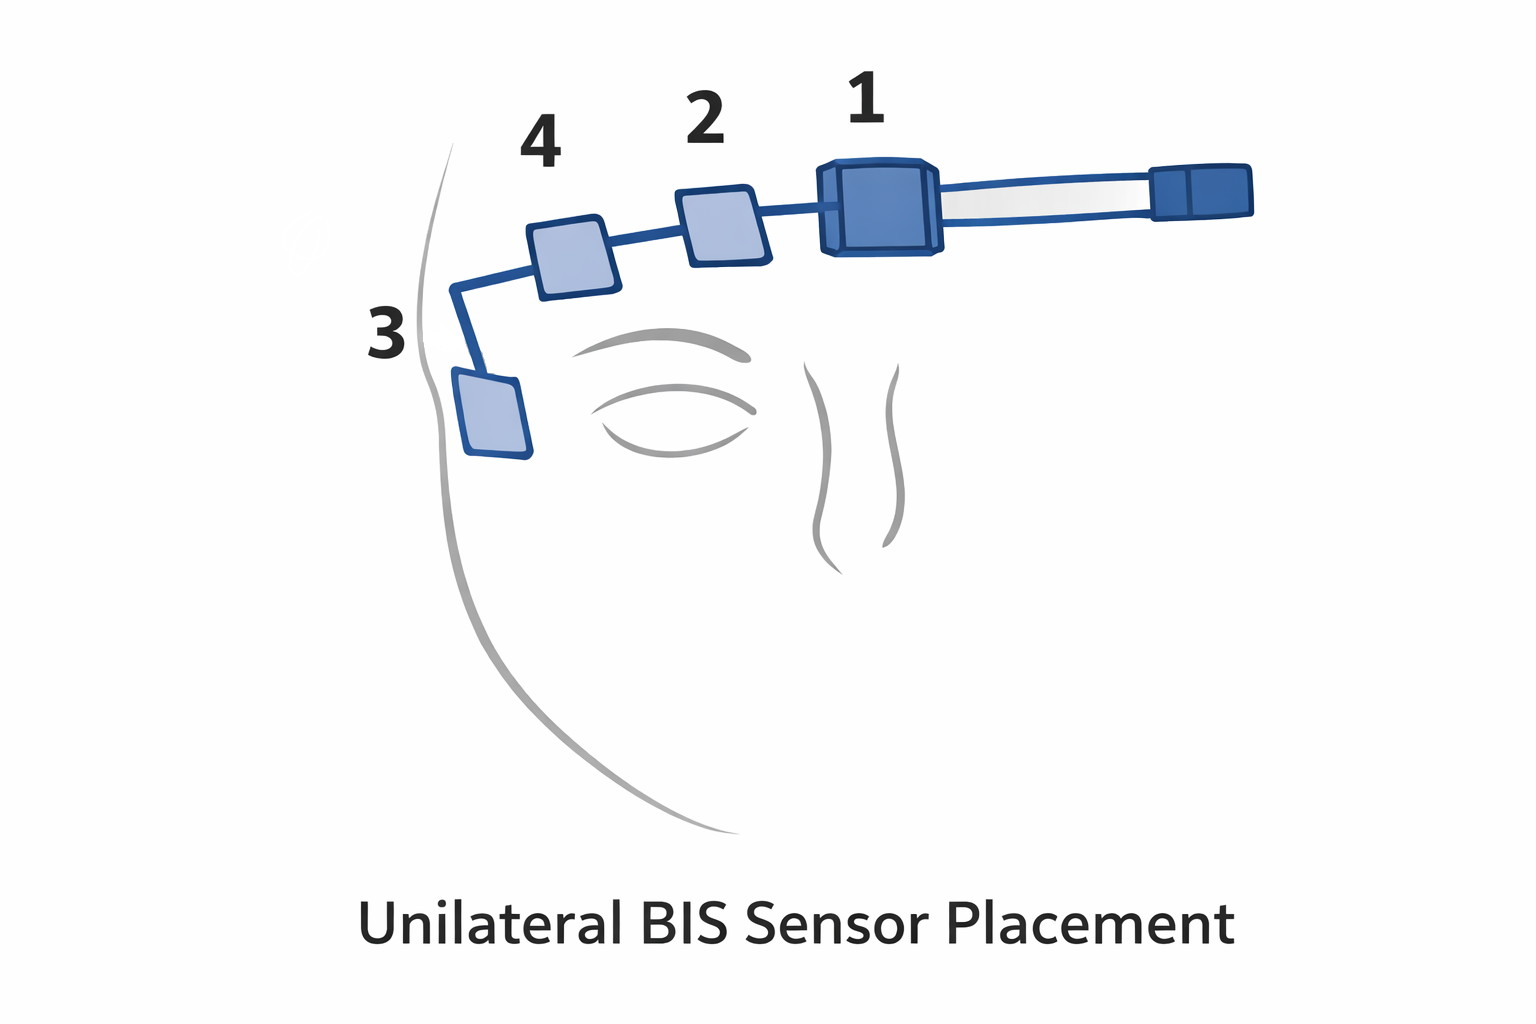
\includegraphics[width=0.65\linewidth,height=\textheight,keepaspectratio]{img/anexo_f_sensor_unilateral.png}

}

\caption{\label{fig-sensor-unilateral}Colocación del sensor empleado en
monitorización unilateral. Elaboración propia a partir de la
documentación técnica recopilada.}

\end{figure}%

En bilateral, el sensor dispone de un electrodo central común
(\texttt{C}), un electrodo de tierra (\texttt{G}) y cuatro electrodos de
lectura: temporal izquierdo (\texttt{LT}), frontal izquierdo
(\texttt{LE}), frontal derecho (\texttt{RE}) y temporal derecho
(\texttt{RT}). Los canales 1 y 2 se obtienen en el lado izquierdo y los
canales 3 y 4 en el derecho.

\begin{figure}

\centering{

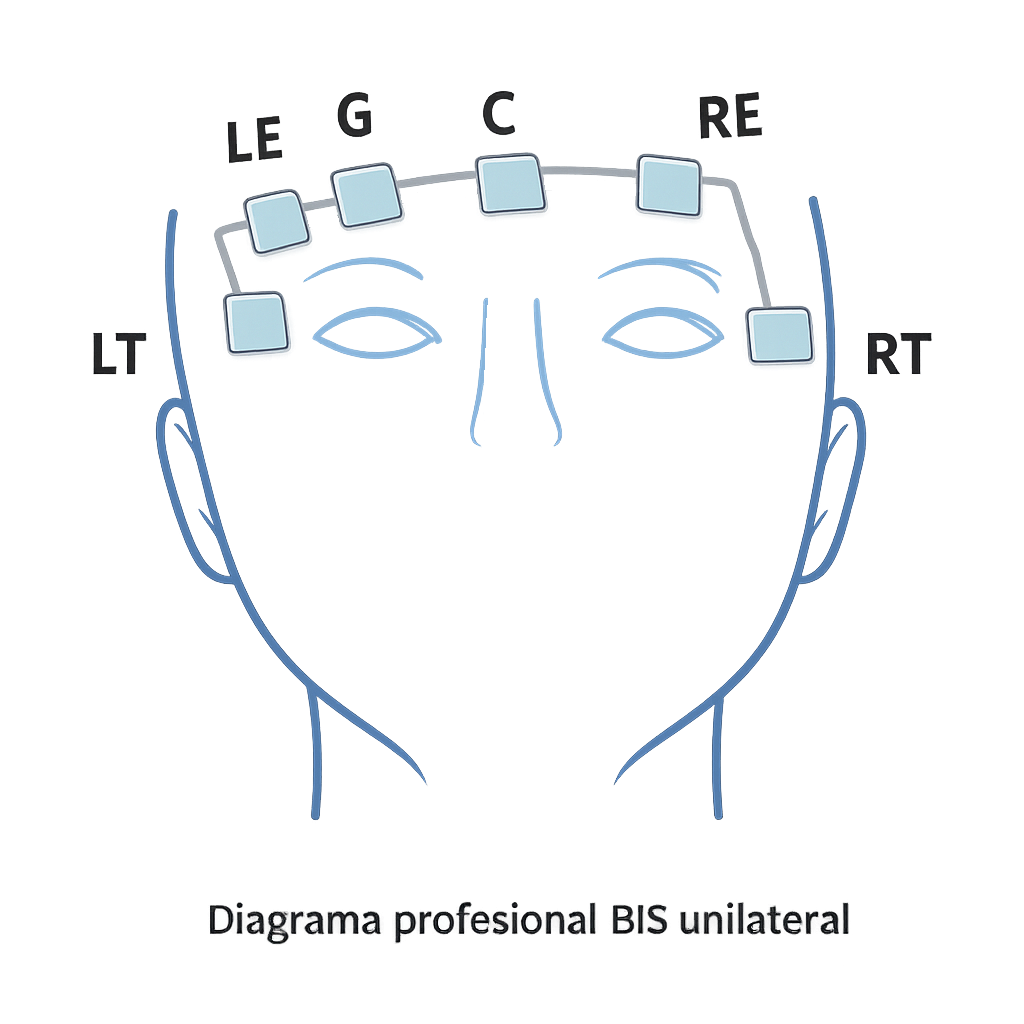
\includegraphics[width=0.55\linewidth,height=\textheight,keepaspectratio]{img/anexo_f_sensor_bilateral.png}

}

\caption{\label{fig-sensor-bilateral}Colocación del sensor empleado en
monitorización bilateral. Elaboración propia a partir de la
documentación técnica recopilada.}

\end{figure}%

En la implementación final, la reconstrucción unilateral utiliza el
canal 1. En bilateral se utiliza el canal 1 para la matriz izquierda y
el canal 3 para la matriz derecha. La especificación técnica del puerto
serie indica que, con un sensor de dos canales, el primer conjunto
espectral válido corresponde al canal 1, mientras que con un sensor de
cuatro canales los dos conjuntos válidos corresponden a los canales 1 y
3 \citep{CovidienSerial2010}.

\begin{longtable}[]{@{}
  >{\raggedright\arraybackslash}p{(\linewidth - 8\tabcolsep) * \real{0.1875}}
  >{\raggedright\arraybackslash}p{(\linewidth - 8\tabcolsep) * \real{0.1875}}
  >{\raggedleft\arraybackslash}p{(\linewidth - 8\tabcolsep) * \real{0.2500}}
  >{\raggedright\arraybackslash}p{(\linewidth - 8\tabcolsep) * \real{0.1875}}
  >{\raggedright\arraybackslash}p{(\linewidth - 8\tabcolsep) * \real{0.1875}}@{}}
\caption{Diferencias principales entre las modalidades de
adquisición}\label{tbl-modalidades-bis}\tabularnewline
\toprule\noalign{}
\begin{minipage}[b]{\linewidth}\raggedright
Modalidad
\end{minipage} & \begin{minipage}[b]{\linewidth}\raggedright
EEG crudo
\end{minipage} & \begin{minipage}[b]{\linewidth}\raggedleft
Canales físicos
\end{minipage} & \begin{minipage}[b]{\linewidth}\raggedright
Bloque procesado del \texttt{.spa}
\end{minipage} & \begin{minipage}[b]{\linewidth}\raggedright
Conjunto espectral
\end{minipage} \\
\midrule\noalign{}
\endfirsthead
\toprule\noalign{}
\begin{minipage}[b]{\linewidth}\raggedright
Modalidad
\end{minipage} & \begin{minipage}[b]{\linewidth}\raggedright
EEG crudo
\end{minipage} & \begin{minipage}[b]{\linewidth}\raggedleft
Canales físicos
\end{minipage} & \begin{minipage}[b]{\linewidth}\raggedright
Bloque procesado del \texttt{.spa}
\end{minipage} & \begin{minipage}[b]{\linewidth}\raggedright
Conjunto espectral
\end{minipage} \\
\midrule\noalign{}
\endhead
\bottomrule\noalign{}
\endlastfoot
Unilateral & \texttt{.r2a} & 2 & Bloque combinado \texttt{Ch\ 12} &
Canal 1 \\
Bilateral & \texttt{.r4a} & 4 & \texttt{Ch\ 1} izquierdo y
\texttt{Ch\ 3} derecho & Canal 1 izquierdo y canal 3 derecho \\
\end{longtable}

\section{Organización de una exportación
BIS}\label{organizaciuxf3n-de-una-exportaciuxf3n-bis}

Los archivos de un mismo registro comparten el nombre base. Por ejemplo,
\texttt{L03041035.r2a}, \texttt{L03041035.h\_a} y \texttt{L03041035.spa}
pertenecen a la misma sesión. La aplicación busca estos archivos de
forma recursiva, comprueba que exista una única exportación y determina
automáticamente la modalidad a partir de la extensión del archivo de
EEG.

\begin{longtable}[]{@{}
  >{\raggedright\arraybackslash}p{(\linewidth - 6\tabcolsep) * \real{0.2500}}
  >{\raggedright\arraybackslash}p{(\linewidth - 6\tabcolsep) * \real{0.2500}}
  >{\raggedright\arraybackslash}p{(\linewidth - 6\tabcolsep) * \real{0.2500}}
  >{\raggedright\arraybackslash}p{(\linewidth - 6\tabcolsep) * \real{0.2500}}@{}}
\caption{Archivos encontrados en las exportaciones BIS
analizadas}\label{tbl-archivos-bis}\tabularnewline
\toprule\noalign{}
\begin{minipage}[b]{\linewidth}\raggedright
Extensión
\end{minipage} & \begin{minipage}[b]{\linewidth}\raggedright
Formato
\end{minipage} & \begin{minipage}[b]{\linewidth}\raggedright
Contenido principal
\end{minipage} & \begin{minipage}[b]{\linewidth}\raggedright
Uso en el proyecto
\end{minipage} \\
\midrule\noalign{}
\endfirsthead
\toprule\noalign{}
\begin{minipage}[b]{\linewidth}\raggedright
Extensión
\end{minipage} & \begin{minipage}[b]{\linewidth}\raggedright
Formato
\end{minipage} & \begin{minipage}[b]{\linewidth}\raggedright
Contenido principal
\end{minipage} & \begin{minipage}[b]{\linewidth}\raggedright
Uso en el proyecto
\end{minipage} \\
\midrule\noalign{}
\endhead
\bottomrule\noalign{}
\endlastfoot
\texttt{.r2a} & Binario & EEG crudo de dos canales & Reconstrucción
unilateral \\
\texttt{.r4a} & Binario & EEG crudo de cuatro canales & Reconstrucción
bilateral \\
\texttt{.h\_a} & Binario & Cabecera y parámetros de adquisición & Número
de canales, frecuencia de muestreo y calibración \\
\texttt{.t\_a} & Texto & Fecha y hora inicial de la señal cruda &
Alineación temporal \\
\texttt{.f\_a} & Texto delimitado & Uno o dos espectros de potencia por
segundo & DSA original del monitor \\
\texttt{.spa} & Texto delimitado & Variables procesadas por segundo &
BIS, SEF, MEF, SQI, potencia y configuración \\
\texttt{.m\_a} & Texto & Revisiones, configuración y mensajes del módulo
& Trazabilidad técnica \\
\texttt{.e\_a} & Texto & Alarmas, avisos y cambios de estado & Contexto
del registro \\
\texttt{.o\_a} & Texto & Información auxiliar asociada al archivo crudo
& Metadatos de exportación \\
\texttt{.ara} & Binario & Información auxiliar interna del sistema & Se
conserva, pero no se interpreta \\
\end{longtable}

No todos los equipos o configuraciones producen archivos con contenido.
En particular, se han encontrado registros en los que \texttt{.f\_a}
existe pero tiene un tamaño de cero bytes. Esta situación es relevante
para el proyecto, porque justifica la reconstrucción de la DSA a partir
del EEG crudo.

\section{\texorpdfstring{Archivos de EEG crudo: \texttt{.r2a} y
\texttt{.r4a}}{Archivos de EEG crudo: .r2a y .r4a}}\label{archivos-de-eeg-crudo-.r2a-y-.r4a}

Los archivos \texttt{.r2a} y \texttt{.r4a} contienen las muestras
digitalizadas del EEG en formato binario. No incluyen una cabecera de
texto ni una marca temporal para cada muestra, por lo que deben
interpretarse junto con \texttt{.h\_a} y \texttt{.t\_a}.

Cada muestra de un canal ocupa 16 bits y se almacena como un entero con
signo en complemento a dos y formato \emph{little endian}. Esto
significa que cada muestra está formada por dos bytes, el byte menos
significativo se encuentra primero en el archivo y el bit más
significativo de la palabra resultante indica el signo. Al desempaquetar
la pareja se obtiene un entero comprendido entre -32768 y 32767.

Las muestras están entrelazadas por instante temporal:

\begin{itemize}
\tightlist
\item
  En \texttt{.r2a}, cada trama contiene una muestra del canal 1 y otra
  del canal 2. Por tanto, una trama ocupa 4 bytes.
\item
  En \texttt{.r4a}, cada trama contiene una muestra de los canales 1, 2,
  3 y 4. Por tanto, una trama ocupa 8 bytes.
\end{itemize}

\begin{figure}

\centering{

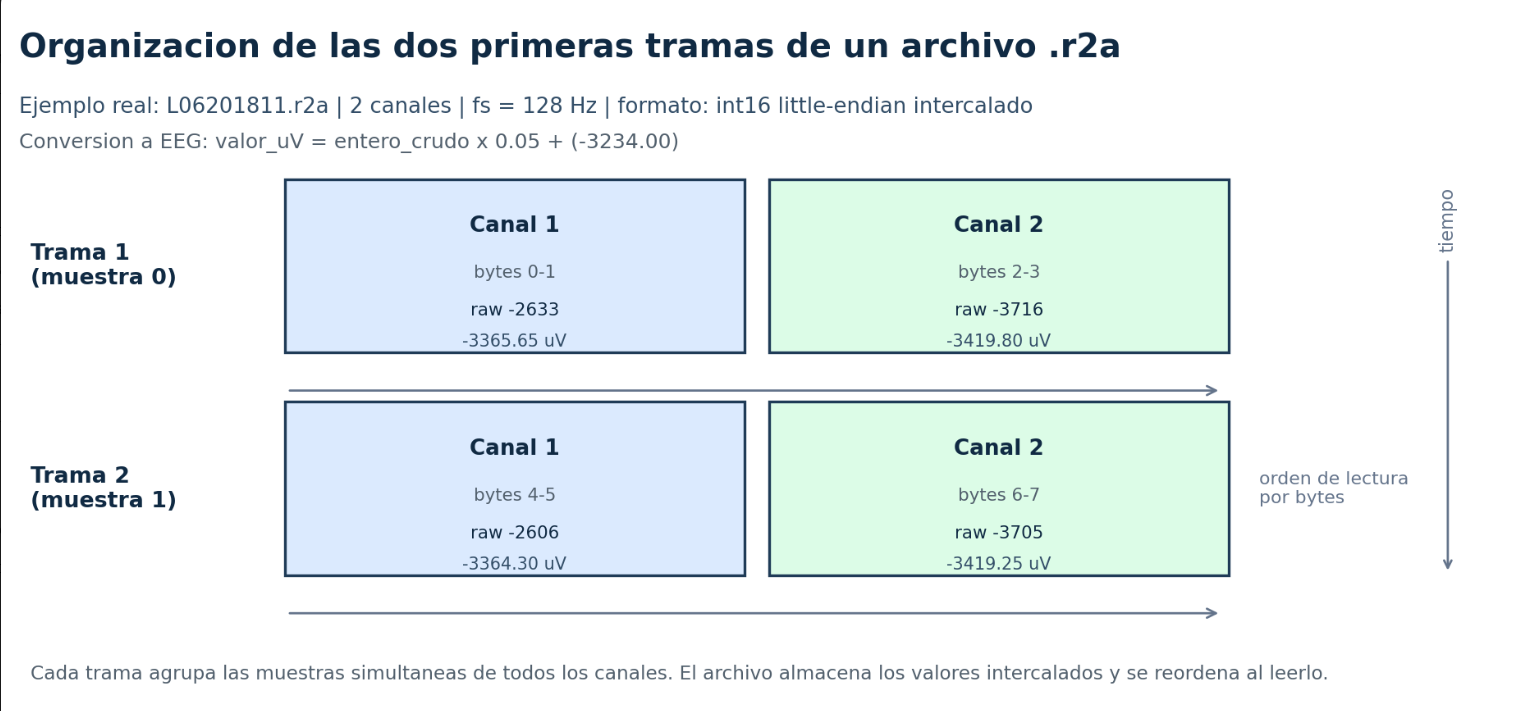
\includegraphics[width=1\linewidth,height=\textheight,keepaspectratio]{img/anexo_f_estructura_r2a.png}

}

\caption{\label{fig-estructura-r2a}Organización de las dos primeras
tramas de un archivo \texttt{.r2a} real.}

\end{figure}%

\begin{figure}

\centering{

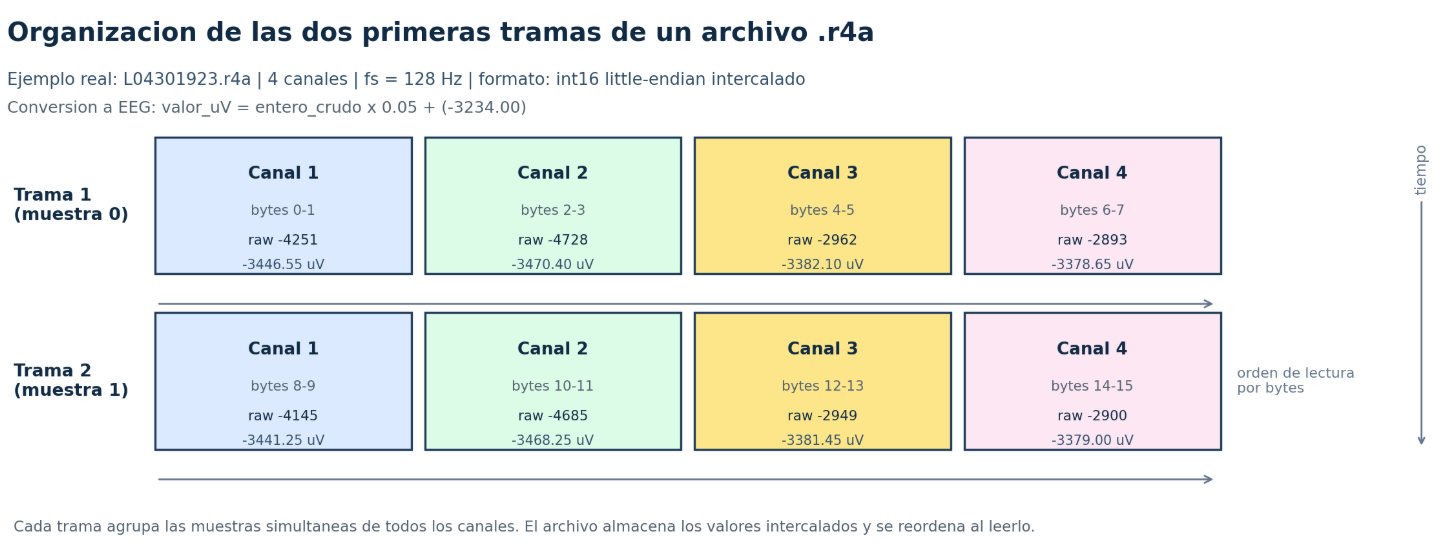
\includegraphics[width=1\linewidth,height=\textheight,keepaspectratio]{img/anexo_f_estructura_r4a.png}

}

\caption{\label{fig-estructura-r4a}Organización de las dos primeras
tramas de un archivo \texttt{.r4a} real.}

\end{figure}%

En las exportaciones utilizadas, la frecuencia de muestreo indicada por
la cabecera es de 128 Hz por canal. Esto implica 128 tramas por segundo
y una resolución temporal entre muestras de 7,8125 ms. La aplicación no
presupone este valor, sino que lo obtiene del archivo \texttt{.h\_a}. La
especificación técnica también describe la transmisión de EEG crudo como
datos entrelazados con una frecuencia de 128 muestras por segundo
\citep{CovidienSerial2010}.

\begin{longtable}[]{@{}
  >{\raggedleft\arraybackslash}p{(\linewidth - 6\tabcolsep) * \real{0.2857}}
  >{\raggedleft\arraybackslash}p{(\linewidth - 6\tabcolsep) * \real{0.2857}}
  >{\raggedright\arraybackslash}p{(\linewidth - 6\tabcolsep) * \real{0.2143}}
  >{\raggedright\arraybackslash}p{(\linewidth - 6\tabcolsep) * \real{0.2143}}@{}}
\caption{Distribución temporal de las tramas a 128
Hz}\label{tbl-tramas-raw}\tabularnewline
\toprule\noalign{}
\begin{minipage}[b]{\linewidth}\raggedleft
Instante dentro del segundo
\end{minipage} & \begin{minipage}[b]{\linewidth}\raggedleft
Trama
\end{minipage} & \begin{minipage}[b]{\linewidth}\raggedright
Contenido de \texttt{.r2a}
\end{minipage} & \begin{minipage}[b]{\linewidth}\raggedright
Contenido de \texttt{.r4a}
\end{minipage} \\
\midrule\noalign{}
\endfirsthead
\toprule\noalign{}
\begin{minipage}[b]{\linewidth}\raggedleft
Instante dentro del segundo
\end{minipage} & \begin{minipage}[b]{\linewidth}\raggedleft
Trama
\end{minipage} & \begin{minipage}[b]{\linewidth}\raggedright
Contenido de \texttt{.r2a}
\end{minipage} & \begin{minipage}[b]{\linewidth}\raggedright
Contenido de \texttt{.r4a}
\end{minipage} \\
\midrule\noalign{}
\endhead
\bottomrule\noalign{}
\endlastfoot
1/128 s & 1 & C1(1), C2(1) & C1(1), C2(1), C3(1), C4(1) \\
2/128 s & 2 & C1(2), C2(2) & C1(2), C2(2), C3(2), C4(2) \\
\ldots{} & \ldots{} & \ldots{} & \ldots{} \\
127/128 s & 127 & C1(127), C2(127) & C1(127), C2(127), C3(127),
C4(127) \\
1 s & 128 & C1(128), C2(128) & C1(128), C2(128), C3(128), C4(128) \\
\end{longtable}

\section{Decodificación y calibración de las
muestras}\label{decodificaciuxf3n-y-calibraciuxf3n-de-las-muestras}

Los enteros almacenados no deben interpretarse directamente como
microvoltios. La cabecera \texttt{.h\_a} contiene una pendiente de
calibración y un offset propios del registro. La implementación
convierte cada muestra mediante la expresión \textbf{EEG (µV) = valor
raw × pendiente + offset}.

Por tanto, el procedimiento completo para cada muestra es:

\begin{enumerate}
\def\labelenumi{\arabic{enumi}.}
\tightlist
\item
  leer la pareja de bytes correspondiente al canal;
\item
  reconstruir la palabra de 16 bits teniendo en cuenta el orden
  \emph{little endian};
\item
  interpretar la palabra como entero con signo en complemento a dos;
\item
  leer la pendiente y el offset de \texttt{.h\_a};
\item
  aplicar la ecuación de calibración.
\end{enumerate}

La Tabla~\ref{tbl-decodificacion-r2a} muestra este proceso sobre las
ocho primeras tramas de un registro real. En cada fila, los dos primeros
bytes corresponden al canal 1 y los dos siguientes al canal 2. En ese
registro, la pendiente almacenada es aproximadamente 0,05 µV por unidad
digital y el offset es -3234 µV. Estos valores se muestran únicamente
como ejemplo: la aplicación los extrae de la cabecera de cada sesión y
no utiliza constantes fijadas manualmente.

\begin{longtable}[]{@{}rlrrrr@{}}
\caption{Ejemplo de decodificación y calibración de un archivo
\protect\texttt{.r2a}}\label{tbl-decodificacion-r2a}\tabularnewline
\toprule\noalign{}
Trama & Bytes de la trama & Raw C1 & Raw C2 & C1 (µV) & C2 (µV) \\
\midrule\noalign{}
\endfirsthead
\toprule\noalign{}
Trama & Bytes de la trama & Raw C1 & Raw C2 & C1 (µV) & C2 (µV) \\
\midrule\noalign{}
\endhead
\bottomrule\noalign{}
\endlastfoot
1 & \texttt{42\ f4\ ce\ f3} & -3006 & -3122 & -3384,30 & -3390,10 \\
2 & \texttt{f2\ f3\ cb\ f2} & -3086 & -3381 & -3388,30 & -3403,05 \\
3 & \texttt{27\ f5\ 24\ f4} & -2777 & -3036 & -3372,85 & -3385,80 \\
4 & \texttt{69\ f4\ d6\ f4} & -2967 & -2858 & -3382,35 & -3376,90 \\
5 & \texttt{1e\ f4\ 0a\ f4} & -3042 & -3062 & -3386,10 & -3387,10 \\
6 & \texttt{46\ f4\ 43\ f4} & -3002 & -3005 & -3384,10 & -3384,25 \\
7 & \texttt{d4\ f4\ d8\ f3} & -2860 & -3112 & -3377,00 & -3389,60 \\
8 & \texttt{db\ f5\ 6e\ f3} & -2597 & -3218 & -3363,85 & -3394,90 \\
\end{longtable}

Si se pierden paquetes de EEG, la especificación indica que el monitor
rellena las muestras ausentes con ceros para mantener la continuidad
temporal \citep{CovidienSerial2010}. Esta circunstancia debe tenerse en
cuenta porque una fila con una proporción elevada de ceros puede
representar una pérdida de información y no una señal EEG
fisiológicamente plana.

\subsection{Diferencias entre unilateral y
bilateral}\label{diferencias-entre-unilateral-y-bilateral}

La estructura numérica es la misma en ambas modalidades; cambia el
número de valores que forman cada trama. En unilateral se obtienen dos
series de EEG de un mismo lado de la frente. En bilateral se obtienen
cuatro series y es posible separar la información de ambos hemisferios.

Para la reconstrucción implementada se emplean:

\begin{itemize}
\tightlist
\item
  canal 1 en los registros unilaterales;
\item
  canal 1 como señal izquierda y canal 3 como señal derecha en los
  registros bilaterales.
\end{itemize}

Los canales 2 y 4 se mantienen en el archivo original, pero no se
utilizan para construir las matrices finales de la aplicación. Esta
decisión es coherente con los conjuntos espectrales identificados por el
fabricante: el primer conjunto corresponde al canal 1 y, en bilateral,
el segundo corresponde al canal 3 \citep{CovidienSerial2010}.

\section{\texorpdfstring{Archivo de cabecera:
\texttt{.h\_a}}{Archivo de cabecera: .h\_a}}\label{archivo-de-cabecera-.h_a}

El archivo \texttt{.h\_a} es una cabecera binaria de tamaño reducido que
describe cómo debe interpretarse la señal cruda. La implementación
extrae de ella, mediante desplazamientos de byte fijos, el número de
canales, la frecuencia de muestreo y los parámetros de calibración
(pendiente y offset):

\begin{longtable}[]{@{}lrl@{}}
\caption{Campos extraídos de la cabecera \protect\texttt{.h\_a} mediante
desplazamientos de byte
fijos}\label{tbl-header-offsets-f}\tabularnewline
\toprule\noalign{}
Parámetro & Offset (byte) & Tipo \\
\midrule\noalign{}
\endfirsthead
\toprule\noalign{}
Parámetro & Offset (byte) & Tipo \\
\midrule\noalign{}
\endhead
\bottomrule\noalign{}
\endlastfoot
Número de canales & 178 & entero corto (16 bits) \\
Frecuencia de muestreo (fs) & 186 & entero (32 bits) \\
Pendiente de calibración & 702 & flotante (32 bits) \\
Offset de calibración & 766 & flotante (32 bits) \\
\end{longtable}

El número de canales también funciona como comprobación de consistencia.
Un registro unilateral debe indicar dos canales y uno bilateral debe
indicar cuatro. Si el valor no coincide con la extensión \texttt{.r2a} o
\texttt{.r4a}, la aplicación detiene la reconstrucción para evitar
interpretar incorrectamente los bytes.

La cabecera puede contener además identificadores de versión del
algoritmo y otros parámetros internos. Estos campos se conservan como
metadatos, pero no son necesarios para la visualización desarrollada.

\section{\texorpdfstring{Archivo temporal:
\texttt{.t\_a}}{Archivo temporal: .t\_a}}\label{archivo-temporal-.t_a}

El archivo \texttt{.t\_a} contiene, en texto, la fecha y hora asociadas
al comienzo de la señal cruda. En los registros analizados consta de una
única línea, por ejemplo:

\begin{Shaded}
\begin{Highlighting}[]
\NormalTok{03/04/2026 10:35:21}
\end{Highlighting}
\end{Shaded}

A partir de este instante, la frecuencia de muestreo y la posición de
cada trama puede asignarse una marca temporal a todas las muestras del
EEG. La aplicación admite las variantes de fecha observadas en las
exportaciones y redondea el instante inicial al segundo.

\section{\texorpdfstring{Archivo de espectros:
\texttt{.f\_a}}{Archivo de espectros: .f\_a}}\label{archivo-de-espectros-.f_a}

El archivo \texttt{.f\_a} contiene la matriz espectral producida por el
monitor. Es un archivo de texto con dos líneas de cabecera y una fila
por segundo. El separador principal es el carácter \texttt{\textbar{}}.

En unilateral su estructura es:

\begin{Shaded}
\begin{Highlighting}[]
\NormalTok{Time | Spectra}
\end{Highlighting}
\end{Shaded}

En bilateral su estructura es:

\begin{Shaded}
\begin{Highlighting}[]
\NormalTok{Time | Left Spectra | Right Spectra}
\end{Highlighting}
\end{Shaded}

Cada campo espectral contiene 60 valores separados por comas,
correspondientes a las frecuencias comprendidas entre 0,5 y 30 Hz, con
incrementos de 0,5 Hz. Al expandir el campo se obtiene una matriz en la
que las filas representan segundos, las columnas representan frecuencias
y cada celda contiene la intensidad espectral.

En las exportaciones estudiadas, los valores aparecen como enteros de
cuatro cifras. La implementación actual los divide entre 100 antes de
representarlos; por ejemplo, \texttt{9356} pasa a \texttt{93,56}. La
unidad y el significado exactos de este escalado se verificarán en la
versión final con la documentación específica del fabricante sobre el
archivo \texttt{.f\_a}. Los manuales de visualización sí confirman que
la DSA mostrada por el monitor representa potencia espectral mediante
una escala de color expresada en decibelios, pero este hecho no basta
por sí solo para demostrar cómo se codifica internamente cada valor del
archivo \citep{CovidienBISadvanced}.

\subsection{Diferencias entre unilateral y
bilateral}\label{diferencias-entre-unilateral-y-bilateral-1}

El archivo unilateral contiene una única columna \texttt{Spectra} y
genera una sola DSA. El bilateral contiene \texttt{Left\ Spectra} y
\texttt{Right\ Spectra}, por lo que se obtienen dos matrices con el
mismo eje temporal y frecuencial. La aplicación representa ambas
matrices con una escala común para que las intensidades puedan
compararse visualmente.

La presencia física del archivo no garantiza que contenga información.
Si \texttt{.f\_a} no existe o está vacío, la aplicación selecciona
automáticamente la reconstrucción desde \texttt{.r2a} o \texttt{.r4a},
siempre que estén disponibles \texttt{.h\_a}, \texttt{.t\_a} y
\texttt{.spa}.

\section{\texorpdfstring{Archivo de variables procesadas:
\texttt{.spa}}{Archivo de variables procesadas: .spa}}\label{archivo-de-variables-procesadas-.spa}

El archivo \texttt{.spa} contiene los parámetros calculados por el
algoritmo BIS y los ajustes de procesamiento del monitor. Se trata de un
archivo de texto delimitado por \texttt{\textbar{}}, normalmente con
resolución de una fila por segundo.

La primera línea agrupa las columnas por canal, la segunda contiene los
nombres de las variables y las siguientes contienen los datos. Algunos
nombres se repiten porque cada bloque de canal exporta el mismo conjunto
de variables. Durante la lectura se generan nombres únicos mediante
sufijos para poder seleccionar el bloque adecuado.

Los valores \texttt{-327.7}, \texttt{-3276}, \texttt{-3276.0},
\texttt{-3276.8}, \texttt{-32767} y \texttt{-32768} se tratan como
códigos centinela de dato no válido y se convierten a valores ausentes.
Esta conversión es necesaria antes de calcular máscaras, estadísticas o
representaciones.

\subsection{Estructura unilateral}\label{estructura-unilateral}

En una exportación unilateral aparecen tres bloques:

\begin{itemize}
\tightlist
\item
  \textbf{\texttt{Ch\ 1}:} variables asociadas al primer canal físico.
\item
  \textbf{\texttt{Ch\ 2}:} canal auxiliar, especialmente sensible a
  determinados artefactos. Varias variables procesadas aparecen como no
  válidas.
\item
  \textbf{\texttt{Ch\ 12}:} bloque combinado generado por el
  procesamiento interno y destinado a la visualización y archivo de los
  resultados finales.
\end{itemize}

La especificación técnica indica expresamente que el conjunto de datos
de \texttt{Ch\ 12} debe utilizarse para mostrar y archivar la
información procesada del modo de dos canales, mientras que el conjunto
de \texttt{Ch\ 2} debe ignorarse \citep{CovidienSerial2010}.

Al convertir los encabezados repetidos en nombres únicos, el tercer
bloque queda identificado habitualmente mediante el sufijo \texttt{\_3}.
Por este motivo, la aplicación prioriza \texttt{SEF08\_3},
\texttt{MEDFRQ08\_3}, \texttt{SQI10\_3}, \texttt{TOTPOW08\_3} y
\texttt{DB13U01\_3}, y los normaliza internamente eliminando el sufijo.

\subsection{Estructura bilateral}\label{estructura-bilateral}

En bilateral aparecen cuatro bloques de variables. Para el análisis se
conservan:

\begin{itemize}
\tightlist
\item
  \textbf{\texttt{Ch\ 1}, sin sufijo:} variables procesadas del
  hemisferio izquierdo.
\item
  \textbf{\texttt{Ch\ 3}, sufijo \texttt{\_3}:} variables procesadas del
  hemisferio derecho.
\end{itemize}

Los bloques \texttt{Ch\ 2} y \texttt{Ch\ 4} contienen información
auxiliar de los canales físicos y numerosos valores centinela para las
variables de alto nivel, por lo que no se utilizan en la visualización
clínica. La modalidad bilateral añade, además, variables que comparan
ambos hemisferios, especialmente \texttt{ASYM09}.

\section{Variables procesadas de mayor
interés}\label{variables-procesadas-de-mayor-interuxe9s}

La tabla Tabla~\ref{tbl-variables-principales} resume las variables del
\texttt{.spa} que tienen una relación directa con el trabajo.

\begin{longtable}[]{@{}
  >{\raggedright\arraybackslash}p{(\linewidth - 6\tabcolsep) * \real{0.2500}}
  >{\raggedright\arraybackslash}p{(\linewidth - 6\tabcolsep) * \real{0.2500}}
  >{\raggedright\arraybackslash}p{(\linewidth - 6\tabcolsep) * \real{0.2500}}
  >{\raggedright\arraybackslash}p{(\linewidth - 6\tabcolsep) * \real{0.2500}}@{}}
\caption{Variables procesadas principales utilizadas por la
aplicación}\label{tbl-variables-principales}\tabularnewline
\toprule\noalign{}
\begin{minipage}[b]{\linewidth}\raggedright
Variable
\end{minipage} & \begin{minipage}[b]{\linewidth}\raggedright
Significado
\end{minipage} & \begin{minipage}[b]{\linewidth}\raggedright
Unidad o rango
\end{minipage} & \begin{minipage}[b]{\linewidth}\raggedright
Utilización en el proyecto
\end{minipage} \\
\midrule\noalign{}
\endfirsthead
\toprule\noalign{}
\begin{minipage}[b]{\linewidth}\raggedright
Variable
\end{minipage} & \begin{minipage}[b]{\linewidth}\raggedright
Significado
\end{minipage} & \begin{minipage}[b]{\linewidth}\raggedright
Unidad o rango
\end{minipage} & \begin{minipage}[b]{\linewidth}\raggedright
Utilización en el proyecto
\end{minipage} \\
\midrule\noalign{}
\endhead
\bottomrule\noalign{}
\endlastfoot
\texttt{DB13U01} & Índice BIS procesado & 0 a 100 & Curva principal de
profundidad de hipnosis \\
\texttt{SQI10} & Índice de calidad de señal & 0 a 100 \% & Exclusión de
segundos con calidad insuficiente \\
\texttt{TOTPOW08} & Potencia total del EEG entre 0,5 y 30 Hz & dB &
Detección de datos espectrales no válidos \\
\texttt{SEF08} & Frecuencia por debajo de la cual se concentra el 95 \%
de la potencia & Hz & Curva superpuesta sobre la DSA \\
\texttt{MEDFRQ08} & Frecuencia mediana, por debajo de la cual se
concentra el 50 \% de la potencia & Hz & Curva MEF superpuesta sobre la
DSA \\
\texttt{SpSmooth} & Código de suavizado espectral configurado & Código
discreto & Selección de la ventana de suavizado de la reconstrucción \\
\texttt{LoFilter} & Código del filtro de baja frecuencia & Código
discreto & Configuración del filtro pasa-altos aplicado al EEG \\
\texttt{ASYM09} & Asimetría de potencia entre hemisferios & Índice
bilateral & Comparación izquierda-derecha \\
\end{longtable}

\subsection{\texorpdfstring{Índice BIS:
\texttt{DB13U01}}{Índice BIS: DB13U01}}\label{uxedndice-bis-db13u01}

Es el índice numérico derivado del EEG que resume el estado hipnótico en
una escala de 0 a 100. En la aplicación se representa bajo la DSA y
comparte su eje temporal. En unilateral se utiliza el valor del bloque
\texttt{Ch\ 12}; en bilateral se representan de forma independiente el
BIS izquierdo y el derecho.

Los valores fuera del intervalo 0-100 y los códigos centinela se
consideran no válidos. Además, el BIS se oculta cuando la matriz del
hemisferio correspondiente ha sido invalidada por falta de calidad.

\subsection{\texorpdfstring{Calidad de señal:
\texttt{SQI10}}{Calidad de señal: SQI10}}\label{calidad-de-seuxf1al-sqi10}

El SQI expresa la calidad o fiabilidad de la señal recibida. Una
disminución puede deberse a mala adherencia del sensor, movimiento,
interferencias o actividad muscular. Es una variable esencial porque
evita interpretar como actividad cerebral válida una señal degradada.

En este proyecto se genera una máscara cuando \texttt{SQI10} es inferior
a 15. Los segundos afectados se eliminan de la DSA y de las curvas
asociadas. El umbral se utiliza como criterio técnico de visualización y
no como una decisión clínica aislada.

\subsection{\texorpdfstring{Potencia total:
\texttt{TOTPOW08}}{Potencia total: TOTPOW08}}\label{potencia-total-totpow08}

Representa la potencia total del EEG en el intervalo espectral de 0,5 a
30 Hz. Resulta útil para comprobar si el monitor dispone de información
espectral válida. Cuando contiene un código centinela, el segundo
correspondiente se excluye.

El análisis conjunto de \texttt{.spa} y \texttt{.f\_a} mostró que muchas
bandas blancas de la DSA coinciden con valores no válidos de
\texttt{TOTPOW08} y con descensos del SQI. Por ello, ambas variables
forman parte de la máscara final.

\subsection{Frecuencias SEF y MEF}\label{frecuencias-sef-y-mef}

\texttt{SEF08} es la frecuencia del borde espectral, definida como la
frecuencia por debajo de la cual se concentra el 95 \% de la potencia.
\texttt{MEDFRQ08} es la frecuencia mediana o MEF, que divide la potencia
acumulada al 50 \%. Ambas se expresan en hercios y permiten resumir cómo
se distribuye la potencia sin reducir toda la información a un único
índice BIS.

La aplicación superpone estas curvas sobre cada DSA. Solo se aceptan
valores entre 0,5 y 30 Hz, que es el intervalo frecuencial representado.

\subsection{\texorpdfstring{Suavizado espectral:
\texttt{SpSmooth}}{Suavizado espectral: SpSmooth}}\label{suavizado-espectral-spsmooth}

\texttt{SpSmooth} codifica la ventana de suavizado configurada en el
monitor. La correspondencia utilizada en el proyecto es:

\begin{longtable}[]{@{}rr@{}}
\caption{Correspondencia empleada para el campo
\protect\texttt{SpSmooth}}\label{tbl-spsmooth}\tabularnewline
\toprule\noalign{}
Código & Ventana \\
\midrule\noalign{}
\endfirsthead
\toprule\noalign{}
Código & Ventana \\
\midrule\noalign{}
\endhead
\bottomrule\noalign{}
\endlastfoot
0 & Sin suavizado adicional \\
1 & 5 s \\
2 & 10 s \\
3 & 30 s \\
4 & 60 s \\
\end{longtable}

En el registro unilateral utilizado como referencia, el código es 3, por
lo que se aplica una media móvil causal de 30 segundos. Así, la ventana
no se elige únicamente por inspección visual, sino a partir de la
configuración exportada por el propio equipo.

\subsection{\texorpdfstring{Filtro de baja frecuencia:
\texttt{LoFilter}}{Filtro de baja frecuencia: LoFilter}}\label{filtro-de-baja-frecuencia-lofilter}

\texttt{LoFilter} indica el corte inferior configurado. La
implementación utiliza la siguiente correspondencia:

\begin{longtable}[]{@{}rr@{}}
\caption{Correspondencia empleada para el campo
\protect\texttt{LoFilter}}\label{tbl-lofilter}\tabularnewline
\toprule\noalign{}
Código & Frecuencia de corte \\
\midrule\noalign{}
\endfirsthead
\toprule\noalign{}
Código & Frecuencia de corte \\
\midrule\noalign{}
\endhead
\bottomrule\noalign{}
\endlastfoot
0 & 0,25 Hz \\
1 & 1 Hz \\
2 & 2 Hz \\
3 & 2,5 Hz \\
\end{longtable}

Durante la reconstrucción se aplica un filtro pasa-altos causal de
primer orden con la frecuencia indicada. Si el campo no está disponible,
se utiliza 0,25 Hz como valor predeterminado y se registra esta
circunstancia en los parámetros del resultado.

\subsection{\texorpdfstring{Asimetría bilateral:
\texttt{ASYM09}}{Asimetría bilateral: ASYM09}}\label{asimetruxeda-bilateral-asym09}

\texttt{ASYM09} solo es relevante en monitorización bilateral y resume
la diferencia de potencia entre ambos hemisferios. Se representa entre
las dos matrices DSA. Para evitar comparaciones engañosas, se invalida
cuando falta la DSA izquierda o la derecha en ese instante.

\section{\texorpdfstring{Otras variables disponibles en
\texttt{.spa}}{Otras variables disponibles en .spa}}\label{otras-variables-disponibles-en-.spa}

El archivo contiene otras variables útiles para interpretar la calidad y
el estado del registro:

\begin{itemize}
\tightlist
\item
  \texttt{SR12}: tasa o porcentaje de supresión del EEG.
\item
  \texttt{BURST}: información sobre brotes de actividad durante patrones
  de supresión.
\item
  \texttt{EMGLOW01}: actividad electromiográfica frontal, que puede
  interferir en el cálculo del BIS.
\item
  \texttt{IMPEDNCE}: información sobre la impedancia y el contacto de
  los electrodos.
\item
  \texttt{BISBIT00}: bits de estado asociados al cálculo del BIS.
\item
  \texttt{SBIS01} y \texttt{SEMG01}: medidas de variabilidad presentes
  en determinadas exportaciones bilaterales.
\item
  \texttt{BiSmooth}, \texttt{NotFiltr}, \texttt{HiFilter} y
  \texttt{PIC\_ID}: parámetros de configuración e identificación del
  sistema.
\end{itemize}

Estas variables se preservan en los archivos originales, pero no todas
se incorporan a la interfaz. La selección final prioriza las que
intervienen en la reconstrucción, en la evaluación de calidad o en la
visualización sincronizada.

\section{Preparación y validación de los
datos}\label{preparaciuxf3n-y-validaciuxf3n-de-los-datos}

La preparación de una sesión sigue los siguientes pasos:

\begin{enumerate}
\def\labelenumi{\arabic{enumi}.}
\tightlist
\item
  Se localiza un único archivo \texttt{.r2a} o \texttt{.r4a} y se
  determina la modalidad.
\item
  Se buscan los archivos con el mismo nombre base.
\item
  Se valida que \texttt{.spa} contenga marcas temporales y las variables
  mínimas.
\item
  Si \texttt{.f\_a} contiene datos, se comprueba que cada espectro
  disponga de 60 valores y que su intervalo temporal sea compatible con
  \texttt{.spa}.
\item
  Si se solicita reconstrucción, se comprueba la disponibilidad de
  \texttt{.h\_a}, \texttt{.t\_a} y la señal cruda.
\item
  Los códigos centinela se convierten en valores ausentes.
\item
  Se crea una línea temporal común con resolución de un segundo.
\end{enumerate}

El \texttt{.spa} se utiliza como línea temporal oficial porque contiene
las variables procesadas que deben aparecer sincronizadas con la DSA.
Los tiempos duplicados se resuelven conservando la última fila recibida
y los huecos se mantienen como valores ausentes, sin interpolar
información clínica.

\section{Tratamiento de la DSA
original}\label{tratamiento-de-la-dsa-original}

Cuando \texttt{.f\_a} está disponible, el procesamiento consiste en:

\begin{enumerate}
\def\labelenumi{\arabic{enumi}.}
\tightlist
\item
  separar la fecha y el campo espectral;
\item
  expandir los 60 valores de frecuencia;
\item
  dividir los valores entre 100 para recuperar la escala en dB;
\item
  asignar las frecuencias de 0,5 a 30 Hz;
\item
  alinear cada fila con el segundo correspondiente de \texttt{.spa};
\item
  aplicar la máscara de calidad.
\end{enumerate}

En bilateral se realiza el mismo proceso para \texttt{Left\ Spectra} y
\texttt{Right\ Spectra}, manteniendo una línea temporal común.

\section{Reconstrucción desde el EEG
crudo}\label{reconstrucciuxf3n-desde-el-eeg-crudo}

Si \texttt{.f\_a} no está disponible, la aplicación reconstruye la DSA
mediante el siguiente procedimiento:

\begin{enumerate}
\def\labelenumi{\arabic{enumi}.}
\tightlist
\item
  lectura de los parámetros de adquisición desde \texttt{.h\_a};
\item
  lectura de la hora inicial desde \texttt{.t\_a};
\item
  separación de los canales entrelazados de \texttt{.r2a} o
  \texttt{.r4a};
\item
  conversión de las muestras utilizando la calibración de la cabecera;
\item
  filtrado pasa-altos según \texttt{LoFilter};
\item
  estimación espectral mediante Welch con ventanas de 2 segundos y
  avance de 1 segundo;
\item
  selección de 0,5 a 30 Hz con resolución de 0,5 Hz;
\item
  conversión a decibelios respecto a la referencia utilizada por el
  proyecto;
\item
  ajuste a la línea temporal de \texttt{.spa};
\item
  suavizado causal según \texttt{SpSmooth};
\item
  aplicación de un desplazamiento temporal empírico de 10 segundos en
  unilateral o 6 segundos en bilateral;
\item
  aplicación de la máscara final.
\end{enumerate}

La máscara considera:

\begin{itemize}
\tightlist
\item
  \texttt{SQI10} inferior a 15;
\item
  \texttt{TOTPOW08} ausente o no válido;
\item
  más del 50 \% de las muestras del EEG crudo iguales a cero dentro de
  un mismo segundo;
\item
  discontinuidades superiores a un segundo;
\item
  filas completamente ausentes después del suavizado y desplazamiento.
\end{itemize}

En bilateral se calcula una máscara independiente para cada hemisferio.
SEF, MF y BIS siguen la máscara de su lado, mientras que \texttt{ASYM09}
requiere que ambas matrices sean válidas. El desarrollo completo de esta
metodología, incluyendo la validación experimental de cada parámetro, se
recoge en el Anexo G.

\section{Plantilla ICCA: estructura y
organización}\label{plantilla-icca-estructura-y-organizaciuxf3n}

Las variables clínicas se reciben en forma de una plantilla Excel
estructurada, con una organización fija que la aplicación asume al
leerla y al generar los archivos auxiliares por sesión. La plantilla se
compone de cuatro hojas:

\begin{longtable}[]{@{}
  >{\raggedright\arraybackslash}p{(\linewidth - 4\tabcolsep) * \real{0.3333}}
  >{\raggedright\arraybackslash}p{(\linewidth - 4\tabcolsep) * \real{0.3333}}
  >{\raggedright\arraybackslash}p{(\linewidth - 4\tabcolsep) * \real{0.3333}}@{}}
\caption{Hojas de la plantilla ICCA y su naturaleza
temporal}\label{tbl-hojas-icca}\tabularnewline
\toprule\noalign{}
\begin{minipage}[b]{\linewidth}\raggedright
Hoja
\end{minipage} & \begin{minipage}[b]{\linewidth}\raggedright
Contenido
\end{minipage} & \begin{minipage}[b]{\linewidth}\raggedright
Naturaleza temporal
\end{minipage} \\
\midrule\noalign{}
\endfirsthead
\toprule\noalign{}
\begin{minipage}[b]{\linewidth}\raggedright
Hoja
\end{minipage} & \begin{minipage}[b]{\linewidth}\raggedright
Contenido
\end{minipage} & \begin{minipage}[b]{\linewidth}\raggedright
Naturaleza temporal
\end{minipage} \\
\midrule\noalign{}
\endhead
\bottomrule\noalign{}
\endlastfoot
\texttt{general} & Contexto del ingreso: identificador, fechas de
ingreso y alta, edad, peso & Estática (una fila por paciente) \\
\texttt{constantes\_vitales} & Frecuencia cardiaca, presión arterial,
SpO₂, temperatura, frecuencia respiratoria, PIC & Mediciones
periódicas \\
\texttt{analisis} & Resultados analíticos: hemoglobina, iones, glucosa,
gasometría & Observaciones puntuales \\
\texttt{perfusiones} & Fármacos en perfusión continua y sus dosis &
Cambios de dosis activa \\
\end{longtable}

En todas las hojas, la fila 3 contiene la cabecera de columnas y los
datos comienzan en la fila 4; este convenio de posición fija es el que
utiliza la aplicación para leer y para reemplazar los datos de cada hoja
sin alterar su formato. Las tres hojas temporales
(\texttt{constantes\_vitales}, \texttt{analisis}, \texttt{perfusiones})
incluyen obligatoriamente una columna \texttt{timestamp}, que es la que
se usa para determinar qué filas corresponden al intervalo de una sesión
BIS concreta. La hoja \texttt{general} incluye, entre otras, las
columnas \texttt{fecha\_hora\_ingreso} y \texttt{fecha\_hora\_alta}, que
delimitan el intervalo temporal completo cubierto por el Excel cuando
están disponibles.

\section{Organización de pacientes y
sesiones}\label{organizaciuxf3n-de-pacientes-y-sesiones}

Además de interpretar los archivos BIS e ICCA de forma aislada, la
aplicación organiza ambas fuentes en una estructura de carpetas por
paciente, generando manifiestos que documentan la procedencia de cada
archivo. Esta sección describe la implementación concreta de dicha
organización.

\subsection{Detección de sesiones BIS y de plantillas ICCA
compatibles}\label{detecciuxf3n-de-sesiones-bis-y-de-plantillas-icca-compatibles}

Antes de crear un paciente, la aplicación localiza automáticamente las
sesiones BIS y las plantillas ICCA disponibles dentro de las carpetas
seleccionadas:

\begin{itemize}
\tightlist
\item
  Para BIS, se recorre recursivamente la carpeta en busca de archivos
  \texttt{.spa}; cada uno define una carpeta de sesión candidata. De esa
  sesión se extrae el intervalo temporal completo (inicio y fin según la
  columna \texttt{Time}), el número de filas, el número de timestamps
  únicos y duplicados, y la modalidad (unilateral o bilateral, deducida
  de si existe un archivo \texttt{.r2a} o \texttt{.r4a} en la misma
  carpeta).
\item
  Para ICCA, se recorre la carpeta en busca de archivos
  \texttt{.xlsx}/\texttt{.xlsm}, y de cada uno se extrae su intervalo
  temporal: primero se intenta a partir de las fechas de ingreso y alta
  de la hoja \texttt{general}; si no están disponibles, se calcula a
  partir del rango de timestamps observado en las hojas temporales.
\end{itemize}

\subsection{Cálculo de solapamiento y compatibilidad
BIS-ICCA}\label{cuxe1lculo-de-solapamiento-y-compatibilidad-bis-icca}

Para cada sesión BIS se calcula su solapamiento temporal con cada
plantilla ICCA candidata: el intervalo de intersección, la proporción de
la duración de la sesión BIS que queda cubierta por el ICCA, y si el
ICCA cubre por completo el intervalo de la sesión. Solo las plantillas
ICCA con solapamiento mayor que cero segundos se consideran compatibles
con esa sesión y se ofrecen como fuente de su archivo auxiliar.

\subsection{Estructura de carpetas y
manifiestos}\label{estructura-de-carpetas-y-manifiestos}

Cada paciente se numera automáticamente siguiendo el patrón
\texttt{PACIENTE\_NNN} (con al menos tres dígitos, incrementando a
partir del último número existente en el directorio de trabajo). Dentro
de la carpeta del paciente:

\begin{itemize}
\tightlist
\item
  \texttt{ICCA\_ORIGINALES/} conserva una copia numerada de cada
  plantilla ICCA de origen, sin modificar.
\item
  \texttt{SESIONES/} contiene una subcarpeta por cada sesión BIS
  asignada, nombrada
  \texttt{SESION\_NNN\_\textless{}identificador\textgreater{}}
  (numeradas según su orden cronológico de inicio). Cada una de estas
  subcarpetas incluye:

  \begin{itemize}
  \tightlist
  \item
    \texttt{BIS/}: copia íntegra de la carpeta de exportación BIS
    original.
  \item
    \texttt{ICCA/}: si existe alguna plantilla ICCA compatible, un Excel
    auxiliar generado específicamente para esa sesión (ver más abajo).
  \end{itemize}
\end{itemize}

Al finalizar la creación, se generan dos tipos de manifiesto en formato
JSON:

\begin{itemize}
\tightlist
\item
  \textbf{\texttt{paciente.json}}, en la raíz del paciente, con el
  identificador del paciente, las fechas de creación y última
  actualización, las rutas originales de todas las fuentes utilizadas y
  un resumen de cada sesión.
\item
  \textbf{\texttt{sesion.json}}, dentro de cada subcarpeta de sesión,
  con el identificador de la sesión BIS, su modalidad, su intervalo
  temporal, la ruta de la exportación BIS original, la referencia al
  Excel ICCA auxiliar (si existe) y el detalle de los solapamientos
  calculados con cada fuente ICCA.
\end{itemize}

Ambos manifiestos permiten reconstruir en cualquier momento de qué
archivos originales procede cada paciente, sin necesidad de volver a
inspeccionar los datos.

\subsection{Generación del Excel ICCA
auxiliar}\label{generaciuxf3n-del-excel-icca-auxiliar}

El Excel auxiliar de cada sesión se genera a partir de la plantilla ICCA
original, conservando su estructura de hojas y su formato de celda. Para
cada una de las tres hojas temporales, se recopilan las filas de todas
las plantillas ICCA compatibles cuyo \texttt{timestamp} cae dentro del
intervalo de la sesión BIS, se eliminan las filas duplicadas y se
ordenan cronológicamente antes de escribirlas; el estilo de celda
(formato numérico, fuente, alineación) se copia de la plantilla original
para que el archivo auxiliar mantenga el mismo aspecto. Cada fila
copiada incorpora además el identificador del paciente y de la sesión
(columnas \texttt{paciente\_id} y \texttt{sesion\_bis\_id}), de forma
que la procedencia de un registro pueda determinarse aunque el Excel
auxiliar se consulte de forma aislada, sin el manifiesto que lo
acompaña. Además, se actualiza la hoja \texttt{general} con el
identificador del paciente y de la sesión, y se añade una hoja
adicional, \texttt{metadata\_sesion}, con un resumen de procedencia
(paciente, sesión BIS, intervalo, modo de monitorización, archivos ICCA
de origen y fecha de generación).

\subsection{Validaciones y robustez}\label{validaciones-y-robustez}

La creación de un paciente incorpora varias comprobaciones para evitar
inconsistencias:

\begin{itemize}
\tightlist
\item
  No se permite asignar al mismo paciente dos sesiones BIS solapadas en
  más de 30 segundos.
\item
  Una sesión BIS o una plantilla ICCA ya asignada a otro paciente no
  puede volver a asignarse; la aplicación identifica el conflicto y
  señala a qué paciente pertenece.
\item
  La construcción de la carpeta del paciente se realiza primero en una
  carpeta temporal oculta; solo si el proceso se completa sin errores se
  renombra a su nombre definitivo. Si algo falla a mitad del proceso, la
  carpeta temporal se elimina y no queda ningún paciente a medio crear.
\item
  Al actualizar un paciente ya existente, la carpeta anterior se
  conserva como respaldo hasta que la nueva versión se ha construido
  correctamente, y solo entonces se sustituye; si la sustitución
  fallara, se restaura el respaldo.
\item
  Los archivos Excel de origen se abren mediante una copia temporal si
  el archivo original está bloqueado (por ejemplo, por estar abierto
  simultáneamente por personal clínico), evitando que esa circunstancia
  impida generar el Excel auxiliar.
\end{itemize}

\section{Preparación de datos ICCA para el
visualizador}\label{preparaciuxf3n-de-datos-icca-para-el-visualizador}

El Excel auxiliar generado por el organizador (ver apartado anterior) no
se representa directamente en el visualizador. Antes de mostrarse, se
somete a un procesamiento adicional orientado a dos objetivos: obtener
una serie temporal de resolución uniforme para las constantes vitales y
decidir, de forma auditable, qué determinaciones de gasometría pueden
mostrarse con garantías.

\subsection{Generación de series sintéticas a resolución de un
segundo}\label{generaciuxf3n-de-series-sintuxe9ticas-a-resoluciuxf3n-de-un-segundo}

Para las constantes vitales, la aplicación genera un archivo derivado
(en formato CSV, acompañado de un \texttt{.meta.json} con información de
auditoría) que contiene una fila por cada segundo del intervalo de la
sesión. Las mediciones reales se colocan exactamente en su segundo de
registro y se conservan sin alterar; los instantes anteriores a la
primera medición real o posteriores a la última no se extrapolan, y
permanecen como valores ausentes. Cada fila incluye una columna
\texttt{series\_reales} que indica qué variables tienen, en ese segundo
concreto, una medición real y no un valor sintético, de forma que el
visualizador pueda distinguir siempre ambos casos al representarlos o al
generar el informe PDF. Este proceso es determinista: generar la serie
sintética dos veces a partir de los mismos datos produce exactamente el
mismo resultado, lo que permite tratarla como un artefacto reproducible
y no como una fuente adicional de variabilidad.

\subsection{Auditoría e inferencia del tipo de
gasometría}\label{auditoruxeda-e-inferencia-del-tipo-de-gasometruxeda}

Las determinaciones de gasometría (pO₂, pCO₂) requieren saber si la
muestra es arterial o venosa para interpretarse correctamente, y esta
información no siempre consta de forma explícita en ICCA. La aplicación
resuelve esta situación mediante un procedimiento de auditoría que, para
cada determinación, decide si puede incluirse en la visualización y con
qué grado de confianza:

\begin{itemize}
\tightlist
\item
  Si la plantilla ICCA indica explícitamente el tipo de gasometría, este
  se respeta y la determinación se incluye con origen ``indicado''.
\item
  Si no se indica explícitamente pero la determinación aparece aislada,
  sin su pareja pO₂/pCO₂ en el mismo instante, se excluye por
  considerarse incompleta.
\item
  Si pO₂ y pCO₂ aparecen juntas en el mismo instante y las marcas
  asociadas a la medición son coherentes entre sí, el tipo de muestra
  puede inferirse con confianza alta a partir de ese contexto.
\item
  Si los indicios disponibles resultan contradictorios o insuficientes
  para una inferencia fiable, la determinación se excluye.
\end{itemize}

En todos los casos, la decisión (inclusión o exclusión, tipo final,
origen de la información y motivo cuando se excluye) queda registrada en
una auditoría propia, de forma que el criterio aplicado a cada dato
pueda revisarse posteriormente. Esta estrategia es más matizada que un
simple descarte ante cualquier ambigüedad: aprovecha el contexto
disponible para recuperar determinaciones interpretables, y solo
descarta aquellas en las que el tipo de muestra no puede establecerse
con garantías suficientes.

\section{Consideraciones clínicas y
limitaciones}\label{consideraciones-cluxednicas-y-limitaciones}

El índice BIS y las variables espectrales son resultados procesados y no
sustituyen la valoración clínica. Un valor numérico solo es
interpretable si la señal tiene calidad suficiente y se consideran
posibles interferencias, especialmente la actividad electromiográfica,
el movimiento y el contacto de los electrodos.

La DSA conserva más información que un índice único porque muestra cómo
se distribuye la potencia entre frecuencias y cómo evoluciona en el
tiempo. Por este motivo, el visualizador combina la matriz con BIS, SEF,
MEF, calidad de señal y, en bilateral, asimetría. La finalidad es
facilitar una revisión retrospectiva estructurada, no reproducir de
forma exacta el algoritmo propietario ni realizar diagnóstico
automático.

%% ══════════════════════════════════════════════════════
%%  APÉNDICE G – Metodología de reconstrucción de la DSA
%% ══════════════════════════════════════════════════════
\apendice{Metodología de reconstrucción de la matriz DSA}
\label{ap:estudio-experimental}

\section{G.1 Objetivo del anexo}\label{g.1-objetivo-del-anexo}

Este anexo describe la metodología implementada para reconstruir la
matriz de densidad espectral (DSA) a partir de los archivos de onda
cruda del monitor BIS. Se explican las funciones principales del módulo
\texttt{reconstruccion.py}, los parámetros empleados, las decisiones
metodológicas adoptadas y las métricas utilizadas para comparar la
matriz reconstruida con la matriz espectral exportada por el monitor
cuando esta se encuentra disponible.

\section{G.2 Parámetros generales de
reconstrucción}\label{g.2-paruxe1metros-generales-de-reconstrucciuxf3n}

Todos los parámetros de la reconstrucción se centralizan en un único
diccionario, \texttt{PARAMETROS\_RECONSTRUCCION}, lo que permite
modificar la configuración sin tocar la lógica de las funciones y deja
constancia explícita de cada decisión adoptada.

\begin{longtable}[]{@{}
  >{\raggedright\arraybackslash}p{(\linewidth - 4\tabcolsep) * \real{0.3000}}
  >{\raggedleft\arraybackslash}p{(\linewidth - 4\tabcolsep) * \real{0.4000}}
  >{\raggedright\arraybackslash}p{(\linewidth - 4\tabcolsep) * \real{0.3000}}@{}}
\caption{Parámetros generales de la reconstrucción, extraídos de
\protect\texttt{PARAMETROS\_RECONSTRUCCION}}\label{tbl-parametros-reconstruccion}\tabularnewline
\toprule\noalign{}
\begin{minipage}[b]{\linewidth}\raggedright
Parámetro
\end{minipage} & \begin{minipage}[b]{\linewidth}\raggedleft
Valor
\end{minipage} & \begin{minipage}[b]{\linewidth}\raggedright
Significado
\end{minipage} \\
\midrule\noalign{}
\endfirsthead
\toprule\noalign{}
\begin{minipage}[b]{\linewidth}\raggedright
Parámetro
\end{minipage} & \begin{minipage}[b]{\linewidth}\raggedleft
Valor
\end{minipage} & \begin{minipage}[b]{\linewidth}\raggedright
Significado
\end{minipage} \\
\midrule\noalign{}
\endhead
\bottomrule\noalign{}
\endlastfoot
\texttt{ventana\_welch\_s} & 2 s & Duración de cada ventana de análisis
espectral \\
\texttt{paso\_welch\_s} & 1 s & Avance entre ventanas consecutivas \\
\texttt{solapamiento\_ventanas\_s} & 1 s & Solapamiento efectivo entre
ventanas \\
\texttt{fmin} & 0,5 Hz & Frecuencia mínima analizada \\
\texttt{fmax} & 30 Hz & Frecuencia máxima analizada \\
\texttt{paso\_frecuencia} & 0,5 Hz & Anchura de cada bin frecuencial \\
\texttt{modo\_welch} & densidad & Welch devuelve PSD en µV²/Hz \\
\texttt{tiempo\_referencia} & centro & La ventana se asigna a su
instante central \\
\texttt{umbral\_sqi} & 15 & Límite mínimo de calidad de señal
(\texttt{SQI10}) \\
\texttt{umbral\_ceros}\(^*\) & 0,9 & Definido en el diccionario de
parámetros, pero no consumido por la función de máscara actualmente en
uso (ver nota tras la tabla) \\
\texttt{aplicar\_mascara\_ceros\_raw} & True & Activa la detección de
pérdidas en el EEG crudo \\
\texttt{umbral\_ceros\_raw} & 0,5 & Segundo de EEG crudo inválido si ≥50
\% de sus muestras son cero \\
\texttt{excluir\_invalidos\_suavizado} & True & Los segundos inválidos
se excluyen del promedio móvil \\
\texttt{referencia\_amplitud\_uv\_rms} & 0,0001 µV RMS & Referencia
usada en la conversión logarítmica a dB \\
\texttt{combinacion\_unilateral} & canal 1 & Canal físico usado en
unilateral \\
\texttt{combinacion\_bilateral} & canal 1 izquierdo, canal 3 derecho &
Canales físicos usados en bilateral \\
\texttt{orden\_filtro\_pasa\_altos} & 1 & Orden del filtro
Butterworth \\
\texttt{filtro\_pasa\_altos\_predeterminado\_hz} & 0,25 Hz & Corte usado
si \texttt{LoFilter} no está disponible en el \texttt{.spa} \\
\texttt{shift\_unilateral\_s} & 10 s & Desplazamiento temporal usado en
unilateral \\
\texttt{shift\_bilateral\_s} & 6 s & Desplazamiento temporal usado en
bilateral \\
\end{longtable}

Nótese que \texttt{umbral\_ceros} (90 \%, aplicado sobre los \emph{bins}
espectrales ya calculados) y \texttt{umbral\_ceros\_raw} (50 \%,
aplicado sobre las muestras de la onda cruda) son dos criterios
distintos y complementarios: el primero detecta espectros degenerados
una vez calculados; el segundo detecta la pérdida de señal en origen,
antes incluso de aplicar Welch (ver G.9).

\(^*\) \emph{Nota:} \texttt{umbral\_ceros} es un parámetro heredado de
una versión anterior del módulo de reconstrucción. La función que
efectivamente calcula la máscara de calidad en la implementación actual
(\texttt{\_calcular\_mascaras\_comunes}) no lo utiliza; el criterio
equivalente que sí está activo es la detección de pérdida de señal en la
onda cruda (\texttt{umbral\_ceros\_raw}, G.9). Se mantiene documentado
aquí porque el parámetro sigue presente en el diccionario de
configuración, aunque no tiene efecto sobre el resultado.

\section{G.3 Lectura de cabecera, tiempo inicial y onda
cruda}\label{g.3-lectura-de-cabecera-tiempo-inicial-y-onda-cruda}

\textbf{Funciones:} \texttt{\_extraer\_parametros\_eeg},
\texttt{\_leer\_raw\_intercalado}, \texttt{\_dar\_forma\_raw},
\texttt{\_interpretar\_inicio\_ta}.

La cabecera \texttt{.h\_a} se lee como un binario y se interpretan
cuatro campos mediante desplazamientos fijos de byte:

\begin{longtable}[]{@{}lrll@{}}
\caption{Campos extraídos de la cabecera \protect\texttt{.h\_a} mediante
desplazamientos de byte fijos}\label{tbl-header-offsets}\tabularnewline
\toprule\noalign{}
Parámetro & Offset (byte) & Tipo & Formato \texttt{struct} \\
\midrule\noalign{}
\endfirsthead
\toprule\noalign{}
Parámetro & Offset (byte) & Tipo & Formato \texttt{struct} \\
\midrule\noalign{}
\endhead
\bottomrule\noalign{}
\endlastfoot
Número de canales & 178 & entero corto & \texttt{\textless{}h} \\
Frecuencia de muestreo (fs) & 186 & entero & \texttt{\textless{}i} \\
Pendiente de calibración & 702 & flotante & \texttt{\textless{}f} \\
Offset de calibración & 766 & flotante & \texttt{\textless{}f} \\
\end{longtable}

Se valida que el número de canales sea 2 (unilateral) o 4 (bilateral) y
que \texttt{fs} sea positivo; en caso contrario se rechaza el archivo.
El archivo \texttt{.t\_a} aporta el instante de inicio de la señal
cruda, que se trunca al segundo.

La señal cruda (\texttt{.r2a}/\texttt{.r4a}) se lee como una secuencia
binaria de enteros de 16 bits con signo (\texttt{\textless{}i2},
\emph{little endian}) y se reorganiza en una matriz de
\texttt{n\_muestras\ ×\ n\_canales}. Si el número total de valores no es
múltiplo exacto del número de canales, la implementación descarta el
resto final en lugar de fallar, evitando así perder todo el registro por
un desajuste de unas pocas muestras sueltas.

\section{G.4 Conversión de la señal cruda a
microvoltios}\label{g.4-conversiuxf3n-de-la-seuxf1al-cruda-a-microvoltios}

\textbf{Función:} \texttt{\_canal\_alineado\_uv}.

Antes del cálculo espectral, las muestras digitales se transforman a
microvoltios utilizando los parámetros de calibración de la cabecera:

\[\text{EEG}_{\mu V} = \text{valor\_crudo} \cdot \text{pendiente} + \text{offset}\]

Esta conversión se realiza ya alineada temporalmente con la timeline
común: la función construye un array del tamaño exacto de la timeline
objetivo, inicializado a \texttt{NaN}, y solo rellena con la conversión
los instantes para los que existe muestra cruda real disponible. Así,
cualquier tramo de la timeline sin cobertura de señal cruda queda
automáticamente como ausencia de información, sin necesidad de una
máscara adicional en este paso.

\section{G.5 Filtro pasa-altos
causal}\label{g.5-filtro-pasa-altos-causal}

\textbf{Funciones:} \texttt{\_extraer\_filtro\_lofilter},
\texttt{\_filtrar\_pasa\_altos\_causal}.

El filtro pasa-altos se aplica antes del cálculo espectral con el
objetivo de atenuar componentes de muy baja frecuencia y deriva de línea
base. Se utiliza un filtro Butterworth causal de primer orden,
implementado con \texttt{scipy.signal.butter} (\texttt{output="sos"}) y
aplicado mediante \texttt{sosfilt}. Al ser causal, cada muestra de
salida depende únicamente de muestras presentes y anteriores, respetando
la dirección temporal de adquisición.

La frecuencia de corte se obtiene de la columna \texttt{LoFilter} del
archivo \texttt{.spa}:

\begin{longtable}[]{@{}rr@{}}
\caption{Correspondencia de códigos
\protect\texttt{LoFilter}}\label{tbl-lofilter-anexo}\tabularnewline
\toprule\noalign{}
Código \texttt{LoFilter} & Frecuencia de corte \\
\midrule\noalign{}
\endfirsthead
\toprule\noalign{}
Código \texttt{LoFilter} & Frecuencia de corte \\
\midrule\noalign{}
\endhead
\bottomrule\noalign{}
\endlastfoot
0 & 0,25 Hz \\
1 & 1,0 Hz \\
2 & 2,0 Hz \\
3 & 2,5 Hz \\
\end{longtable}

Si la columna \texttt{LoFilter} no está disponible en el \texttt{.spa},
se emplea 0,25 Hz como valor predeterminado y se registra esta
circunstancia en los parámetros del resultado (campo
\texttt{lofilter\_origen}).

Un detalle metodológico relevante es el tratamiento de los huecos: la
señal puede contener tramos de \texttt{NaN} (por ejemplo, donde la
alineación con la timeline no dispuso de muestra cruda). En lugar de
filtrar la señal completa arrastrando esos huecos, la implementación
localiza los bloques de valores finitos y filtra cada bloque de forma
independiente, con su propio estado inicial del filtro
(\texttt{sosfilt\_zi}). De este modo, un hueco no contamina con
transitorios de filtro los tramos válidos situados antes o después de
él, y los valores no finitos permanecen como ausencia de información en
la salida.

\subsection{Ejemplo numérico del
filtrado}\label{ejemplo-numuxe9rico-del-filtrado}

Para ilustrar el funcionamiento del filtro, se toma un caso concreto:
frecuencia de muestreo \(f_s = 128\) Hz, frecuencia de corte
\(f_c = 2,5\) Hz (código \texttt{LoFilter} 3) y orden 1.

Para un filtro Butterworth pasa-altos digital de primer orden diseñado
mediante transformación bilineal, los coeficientes pueden expresarse a
partir de:

\[K = \tan\left(\frac{\pi f_c}{f_s}\right)\]

Sustituyendo los valores del caso:

\[K = \tan\left(\frac{\pi \cdot 2{,}5}{128}\right) = \tan(0{,}0614) \approx 0{,}0614\]

A partir de \(K\) se obtienen los coeficientes del filtro:

\[b_0 = \frac{1}{1+K} \approx 0{,}9412 \qquad b_1 = \frac{-1}{1+K} \approx -0{,}9412 \qquad a_1 = \frac{K-1}{K+1} \approx -0{,}8842\]

La ecuación recursiva del filtro es:

\[y[n] = b_0\,x[n] + b_1\,x[n-1] - a_1\,y[n-1] = 0{,}9412\,(x[n]-x[n-1]) + 0{,}8842\,y[n-1]\]

Esta expresión es la que relaciona la salida filtrada \(y[n]\) con la
muestra de entrada actual \(x[n]\), la muestra de entrada anterior
\(x[n-1]\) y la propia salida anterior \(y[n-1]\); por ello es una
ecuación recursiva, y la dependencia de \(y[n-1]\) es la que da lugar al
comportamiento de suavizado característico de un filtro Butterworth de
primer orden. El término \(x[n]-x[n-1]\) explica el carácter pasa-altos:
cuando la señal cambia lentamente, esta diferencia es pequeña y la
salida queda muy atenuada; cuando cambia rápidamente, la diferencia es
mayor y esa componente se conserva en mayor medida.

Para la primera muestra de un bloque no existen \(x[-1]\) ni \(y[-1]\).
La implementación resuelve esto con
\texttt{zi\ =\ sosfilt\_zi(sos)\ *\ segmento{[}0{]}}, que inicializa el
filtro como si, antes de la primera muestra, la señal hubiese
permanecido constante en su valor inicial. Como una señal constante
corresponde a una componente de 0 Hz, un filtro pasa-altos debe producir
para ella una salida estacionaria aproximadamente nula; esta
inicialización reduce el transitorio artificial que aparecería al
comienzo del filtrado si se partiera, por ejemplo, de un estado en
reposo.

Tomando como entrada, a modo de ejemplo, cinco muestras en µV y fijando
\(y[0]=0\) por simplicidad:

\begin{longtable}[]{@{}rrr@{}}
\caption{Ejemplo numérico del filtrado pasa-altos
causal}\label{tbl-ejemplo-filtro}\tabularnewline
\toprule\noalign{}
\(n\) & \(x[n]\) (µV) & \(y[n]\) (µV) \\
\midrule\noalign{}
\endfirsthead
\toprule\noalign{}
\(n\) & \(x[n]\) (µV) & \(y[n]\) (µV) \\
\midrule\noalign{}
\endhead
\bottomrule\noalign{}
\endlastfoot
0 & 100 & 0 \\
1 & 102 & 1,88 \\
2 & 104 & 3,55 \\
3 & 103 & 2,19 \\
4 & 101 & 0,06 \\
\end{longtable}

Por ejemplo, la segunda muestra se obtiene como
\(y[1] = 0{,}9412\cdot(102-100) + 0{,}8842\cdot 0 = 1{,}88\) µV, y la
tercera como
\(y[2] = 0{,}9412\cdot(104-102) + 0{,}8842\cdot 1{,}88 = 3{,}55\) µV, y
así sucesivamente. En el proyecto estos coeficientes no se calculan ni
se codifican manualmente, sino que los obtiene
\texttt{scipy.signal.butter} a partir de la frecuencia de corte y de la
frecuencia de muestreo; la expresión de \(K\) se incluye aquí únicamente
para explicar su origen matemático. El filtrado se aplica después con
\texttt{scipy.signal.sosfilt}, por lo que es causal: cada muestra
filtrada depende de la muestra actual, de muestras previas y del estado
previo del filtro, sin utilizar en ningún momento muestras futuras.

\section{G.6 Reconstrucción espectral mediante
Welch}\label{g.6-reconstrucciuxf3n-espectral-mediante-welch}

\textbf{Funciones:} \texttt{\_welch\_por\_bloques},
\texttt{\_reconstruir\_lado}.

\begin{longtable}[]{@{}
  >{\raggedright\arraybackslash}p{(\linewidth - 2\tabcolsep) * \real{0.5000}}
  >{\raggedright\arraybackslash}p{(\linewidth - 2\tabcolsep) * \real{0.5000}}@{}}
\caption{Configuración de la estimación espectral mediante
Welch}\label{tbl-welch-config}\tabularnewline
\toprule\noalign{}
\begin{minipage}[b]{\linewidth}\raggedright
Parámetro
\end{minipage} & \begin{minipage}[b]{\linewidth}\raggedright
Justificación
\end{minipage} \\
\midrule\noalign{}
\endfirsthead
\toprule\noalign{}
\begin{minipage}[b]{\linewidth}\raggedright
Parámetro
\end{minipage} & \begin{minipage}[b]{\linewidth}\raggedright
Justificación
\end{minipage} \\
\midrule\noalign{}
\endhead
\bottomrule\noalign{}
\endlastfoot
Ventana de 2 s & Compromiso entre resolución temporal y frecuencial \\
Avance de 1 s & Permite obtener una estimación por segundo \\
Ventana Hann & Reduce la fuga espectral \\
\texttt{detrend="constant"} & Elimina el valor medio de cada ventana \\
\texttt{scaling="density"} & Obtiene PSD en µV²/Hz \\
Rango 0,5-30 Hz & Rango representado por la DSA del BIS \\
Bin de 0,5 Hz & Resolución frecuencial de la matriz \\
Referencia temporal central & Cada ventana se asigna a su instante
central \\
\end{longtable}

\subsection{De la señal discreta a la resolución de 0,5
Hz}\label{de-la-seuxf1al-discreta-a-la-resoluciuxf3n-de-05-hz}

El EEG no llega al ordenador como una señal continua, sino como una
secuencia finita de muestras. Por eso el análisis frecuencial no puede
usar la Transformada de Fourier continua, sino su versión para señales
muestreadas y finitas, la Transformada Discreta de Fourier (DFT); la FFT
(\emph{Fast Fourier Transform}) no es una transformada distinta, sino el
algoritmo con el que se calcula esa misma DFT de forma mucho más rápida,
y es lo que usa internamente \texttt{scipy.signal.welch}.

La resolución frecuencial que se obtiene de una ventana de \(N\)
muestras a una frecuencia de muestreo \(f_s\) es:

\[\Delta f = \frac{f_s}{N}\]

Con los parámetros de este proyecto (\(f_s = 128\) Hz, \(N = 256\)
muestras por ventana de 2 s):

\[\Delta f = \frac{128}{256} = 0{,}5\ \text{Hz}\]

Este resultado no es casual: es precisamente la razón por la que la
ventana de 2 segundos permite obtener directamente bins de 0,5 Hz, sin
necesidad de ningún ajuste adicional
(\texttt{nfft\ =\ fs\ /\ paso\_frecuencia} en la implementación, ver
G.2).

La misma relación impone también un límite superior a las frecuencias
analizables, la frecuencia de Nyquist:

\[f_{Nyquist} = \frac{f_s}{2} = \frac{128}{2} = 64\ \text{Hz}\]

El rango representado en la DSA (0,5-30 Hz) queda muy por debajo de ese
límite, por lo que la resolución del muestreo no supone ninguna
restricción práctica. La componente de 0 Hz, además, no se incluye en la
matriz resultante, en línea con la eliminación de la media descrita más
abajo: ambas decisiones evitan que un posible desplazamiento constante
de la señal se confunda con actividad oscilatoria real.

Por último, que se use la FFT y no la DFT calculada de forma directa no
es un detalle menor a la escala de este proyecto: el coste de la DFT
directa crece con el cuadrado del número de muestras analizadas,
mientras que la FFT lo reduce a un crecimiento casi lineal. Esa
diferencia es la que permite reconstruir la DSA de un registro de varias
horas completas en un tiempo razonable, en vez de estar limitados a unos
pocos segundos de señal.

Para cada canal, la señal se procesa por segmentos de 2 segundos, a los
que se aplican dos correcciones antes del cálculo espectral propiamente
dicho:

\begin{itemize}
\tightlist
\item
  \textbf{Eliminación de la media (\texttt{detrend="constant"}).} Cada
  segmento se centra en torno a cero, eliminando su nivel medio sin
  alterar sus oscilaciones. Si el fragmento tuviese un desplazamiento
  constante respecto a cero (una componente de continua), la FFT lo
  interpretaría como una gran cantidad de potencia concentrada en 0 Hz,
  una potencia artificial que no corresponde a actividad oscilatoria
  real y que podría contaminar la lectura de las frecuencias más bajas.
\item
  \textbf{Ventana Hann.} Suaviza progresivamente la amplitud del
  segmento hacia sus dos extremos. La FFT asume implícitamente que el
  fragmento analizado se repite de forma periódica; si el principio y el
  final del segmento no encajan entre sí, aparece un salto artificial en
  ese punto de unión. Ese salto, al descomponerse en frecuencias, se
  parece a componentes de alta frecuencia y añade potencia que no está
  realmente presente en el EEG. La ventana Hann atenúa los bordes para
  reducir ese salto y, con ello, la fuga espectral que provocaría.
\end{itemize}

La implementación no llama a \texttt{scipy.signal.welch} sobre la señal
completa con su parámetro de solapamiento interno. En su lugar, extrae
manualmente segmentos de 256 muestras (2 s a 128 Hz) con un
desplazamiento de 128 muestras (1 s) entre inicios consecutivos ---lo
que produce el solapamiento efectivo del 50 \% entre ventanas---, y
aplica \texttt{welch} de forma independiente a cada segmento ya
extraído, con \texttt{noverlap=0} y
\texttt{nfft\ =\ fs\ /\ paso\_frecuencia}. El resultado equivale a un
periodograma modificado (ventana Hann) por segmento, calculado con el
avance deseado; esta equivalencia es la que se comprueba
experimentalmente en la sección G.15.1 frente a
\texttt{scipy.signal.spectrogram}.

Sobre la selección de canales: en registros unilaterales se utiliza el
canal 1 (índice 0). En registros bilaterales,
\texttt{\_reconstruir\_lado} se invoca por separado para el canal 1
(izquierdo) y el canal 3 (derecho); los canales 2 y 4 no intervienen en
la reconstrucción final.

\section{G.7 Conversión de densidad espectral a
dB}\label{g.7-conversiuxf3n-de-densidad-espectral-a-db}

\textbf{Función:} \texttt{\_convertir\_potencia\_a\_db}.

\subsection{De la FFT a la densidad espectral de
potencia}\label{de-la-fft-a-la-densidad-espectral-de-potencia}

Para cada segmento, la FFT devuelve un valor complejo por frecuencia,
formado por una magnitud (cuánta cantidad de esa frecuencia contiene la
señal) y una fase (en qué punto de su ciclo se encuentra esa
componente). El flujo hasta llegar a la densidad espectral de potencia
(PSD) es el siguiente:

\begin{enumerate}
\def\labelenumi{\arabic{enumi}.}
\tightlist
\item
  \textbf{Fragmento de EEG}, \(x(t)\), en µV.
\item
  \textbf{FFT}: para cada frecuencia analizada (0,5 Hz, 1 Hz, \ldots, 30
  Hz) se obtiene una amplitud compleja \(X(f)\).
\item
  \textbf{Potencia}: se toma el módulo al cuadrado de esa amplitud,
  \(P(f) = |X(f)|^2\); al elevar al cuadrado una magnitud en µV, el
  resultado queda en µV².
\item
  \textbf{Densidad espectral de potencia}: para expresar cuánta potencia
  hay por hercio, el resultado se normaliza por el ancho de banda
  analizado y por la ventana empleada, obteniendo \(\text{PSD}(f)\) en
  µV²/Hz. Este es precisamente el resultado que devuelve
  \texttt{scipy.signal.welch} con \texttt{scaling="density"}.
\end{enumerate}

\subsection{Integración por bin y paso a
decibelios}\label{integraciuxf3n-por-bin-y-paso-a-decibelios}

Dado que Welch devuelve densidad espectral de potencia (µV²/Hz) y cada
columna de la DSA representa un intervalo de 0,5 Hz, cada celda se
integra multiplicando por la anchura del bin para recuperar una potencia
aproximada en µV²:

\[\text{potencia\_bin} = \text{PSD} \cdot 0{,}5\ \text{Hz}\]

Posteriormente se aplica una conversión logarítmica respecto a una
referencia de amplitud:

\[\text{DSA}_{dB} = 10 \cdot \log_{10}\!\left(\frac{\text{potencia\_bin} + 10^{-12}}{(0{,}0001\ \mu V)^2}\right)\]

El término \(10^{-12}\) se añade únicamente para evitar problemas
numéricos al calcular el logaritmo de valores nulos, y su magnitud es lo
bastante pequeña como para no alterar de forma perceptible ninguna celda
con señal real.

La referencia del fabricante se expresa como una amplitud, 0,0001 µV
RMS, mientras que lo que se compara en la fórmula es una potencia. Por
ello la referencia debe elevarse al cuadrado,
\((0{,}0001\ \mu V)^2 = 10^{-8}\ \mu V^2\), antes de dividir; el
resultado es equivalente a haber trabajado directamente con amplitudes y
una expresión en \(20 \log_{10}\). Esta referencia se mantiene constante
en toda la aplicación para asegurar la comparabilidad entre registros y
permitir la comparación con la DSA exportada por el monitor.

Para la representación gráfica se emplea la escala lineal fija de 49 a
94 dB especificada por el fabricante (ver G.2). Los valores que quedan
fuera de ese intervalo no se eliminan ni se invalidan: se saturan en los
extremos de la escala cromática, de modo que una celda con una potencia
superior a 94 dB se muestra igual que una de exactamente 94 dB, y
análogamente en el extremo inferior.

\section{G.8 Alineación temporal de la DSA
reconstruida}\label{g.8-alineaciuxf3n-temporal-de-la-dsa-reconstruida}

\textbf{Funciones:} \texttt{\_ajustar\_reconstruida\_a\_timeline},
\texttt{\_alinear\_spa}, \texttt{\_calcular\_indices\_alineacion}.

Welch produce tiempos relativos al inicio de la señal analizada. Estos
tiempos se convierten a marcas temporales absolutas tomando como
referencia el inicio de la timeline común, y la matriz se reindexa sobre
dicha timeline, de forma que cada fila de la DSA reconstruida
corresponda al mismo segundo que las variables procesadas del
\texttt{.spa}. Si el proceso genera marcas temporales duplicadas, se
conserva la última aparición. El \texttt{.spa} se alinea de forma
equivalente sobre la misma timeline mediante \texttt{\_alinear\_spa}.

\section{G.9 Máscaras de calidad}\label{g.9-muxe1scaras-de-calidad}

\textbf{Funciones:} \texttt{\_detectar\_perdidas\_raw\_por\_segundo},
\texttt{\_proyectar\_mascara\_raw\_a\_timeline\_dsa},
\texttt{\_crear\_mascara\_raw\_para\_canal},
\texttt{\_calcular\_mascaras\_comunes},
\texttt{\_calcular\_mascara\_final\_comun}.

Un segundo de la timeline común se considera no válido cuando se cumple
alguno de los siguientes criterios:

\begin{longtable}[]{@{}
  >{\raggedright\arraybackslash}p{(\linewidth - 2\tabcolsep) * \real{0.5000}}
  >{\raggedright\arraybackslash}p{(\linewidth - 2\tabcolsep) * \real{0.5000}}@{}}
\caption{Criterios que componen la máscara de
calidad}\label{tbl-criterios-mascara}\tabularnewline
\toprule\noalign{}
\begin{minipage}[b]{\linewidth}\raggedright
Máscara
\end{minipage} & \begin{minipage}[b]{\linewidth}\raggedright
Criterio
\end{minipage} \\
\midrule\noalign{}
\endfirsthead
\toprule\noalign{}
\begin{minipage}[b]{\linewidth}\raggedright
Máscara
\end{minipage} & \begin{minipage}[b]{\linewidth}\raggedright
Criterio
\end{minipage} \\
\midrule\noalign{}
\endhead
\bottomrule\noalign{}
\endlastfoot
Calidad \texttt{.spa} & \texttt{SQI10\ \textless{}\ 15} o
\texttt{TOTPOW08} ausente \\
Pérdida de señal cruda & ≥50 \% de las muestras del segundo, en el canal
correspondiente, son exactamente cero \\
Segundo incompleto & La alineación no dispuso del conjunto completo de
128 muestras crudas para ese segundo (p.~ej. en los bordes del
registro) \\
Discontinuidades & Segundo ausente en la timeline del \texttt{.spa} o,
si existe, del \texttt{.f\_a} \\
Sin ventana Welch & No existe ninguna ventana de Welch cuyo instante
central caiga en ese segundo (ocurre en el margen inicial que exige la
ventana de 2 s) \\
Hemisferios (bilateral) & Cada hemisferio tiene su propia máscara;
\texttt{ASYM09} se invalida cuando falta información válida en
cualquiera de los dos lados \\
\end{longtable}

El criterio de \textbf{pérdida de señal cruda} se basa en que, ante la
pérdida de paquetes de EEG, el propio equipo rellena las muestras
ausentes con ceros para mantener la continuidad temporal
\citep{CovidienSerial2010}. Los ceros aislados y esporádicos, que no
alcanzan ese 50 \%, no invalidan el segundo. Esta máscara se calcula
sobre el EEG crudo y después se proyecta a la resolución de las ventanas
de Welch: una ventana se invalida si incorpora aunque sea una muestra
perteneciente a un segundo crudo ya marcado como inválido, ya que la
estimación espectral no admite valores ausentes.

La máscara final que efectivamente se aplica a la visualización no es
únicamente la máscara base anterior. Antes de mostrarse, se calcula una
\textbf{disponibilidad} por segundo: cuántos de los últimos
\texttt{SpSmooth} segundos (ver G.10) tenían datos válidos según la
máscara base. Tras aplicar el desplazamiento temporal (G.11) a esa
disponibilidad, un segundo se marca como no representable si, una vez
desplazada, no queda ningún dato válido dentro de su ventana de
suavizado. La máscara final es, por tanto, la unión de la máscara base y
la ausencia de disponibilidad tras suavizado y desplazamiento. Esto es
lo que justifica que, en la práctica, los primeros segundos de cualquier
reconstrucción bilateral o unilateral aparezcan siempre en blanco: no
existe todavía suficiente historia disponible para calcular ni el
suavizado ni aplicarle el desplazamiento.

En registros bilaterales, todos estos criterios (salvo la calidad
\texttt{.spa}, que usa las columnas \texttt{\_izq}/\texttt{\_der}
correspondientes) se calculan de forma independiente para cada
hemisferio.

\section{\texorpdfstring{G.10 Suavizado temporal mediante
\texttt{SpSmooth}}{G.10 Suavizado temporal mediante SpSmooth}}\label{g.10-suavizado-temporal-mediante-spsmooth}

\textbf{Función:} \texttt{\_suavizar\_y\_desplazar}.

\begin{longtable}[]{@{}rr@{}}
\caption{Correspondencia de códigos
\protect\texttt{SpSmooth}}\label{tbl-spsmooth-anexo}\tabularnewline
\toprule\noalign{}
Código \texttt{SpSmooth} & Ventana \\
\midrule\noalign{}
\endfirsthead
\toprule\noalign{}
Código \texttt{SpSmooth} & Ventana \\
\midrule\noalign{}
\endhead
\bottomrule\noalign{}
\endlastfoot
0 & 0 s (sin suavizado) \\
1 & 5 s \\
2 & 10 s \\
3 & 30 s \\
4 & 60 s \\
\end{longtable}

El suavizado se aplica mediante una media móvil causal
(\texttt{rolling}, \texttt{center=False}) con \texttt{min\_periods=1},
de modo que cada segundo se calcula utilizando únicamente valores
presentes y anteriores, y no exige que la ventana esté completamente
llena para producir un resultado. Los segundos marcados como inválidos
por la máscara base se sustituyen por \texttt{NaN} antes del suavizado
(cuando \texttt{excluir\_invalidos\_suavizado=True}, que es el valor por
defecto), evitando así que contribuyan al promedio temporal.

La existencia del parámetro \texttt{SpSmooth} procede de la estructura
exportada por el monitor BIS. La forma exacta del suavizado interno del
equipo no es pública, por lo que la media móvil causal se adopta como
aproximación reproducible y coherente con el carácter temporal del
parámetro, sin pretender reproducir exactamente el algoritmo
propietario.

\section{G.11 Desplazamiento temporal
aplicado}\label{g.11-desplazamiento-temporal-aplicado}

\textbf{Función:} \texttt{\_suavizar\_y\_desplazar}.

\begin{longtable}[]{@{}lr@{}}
\caption{Desplazamiento temporal aplicado tras el
suavizado}\label{tbl-shift-anexo}\tabularnewline
\toprule\noalign{}
Modo & Shift \\
\midrule\noalign{}
\endfirsthead
\toprule\noalign{}
Modo & Shift \\
\midrule\noalign{}
\endhead
\bottomrule\noalign{}
\endlastfoot
Unilateral & 10 s \\
Bilateral & 6 s \\
\end{longtable}

Tras el suavizado se aplica un desplazamiento temporal fijo. Este
desplazamiento no se interpreta como un parámetro fisiológico, sino como
una corrección empírica destinada a mejorar la correspondencia temporal
entre la DSA reconstruida y la DSA exportada por el monitor. Los valores
utilizados fueron seleccionados tras comparar diferentes desplazamientos
(0-30 s) y evaluar las métricas de similitud frente al archivo
\texttt{.f\_a} (ver G.15.2); no se emplea ninguna referencia
bibliográfica para justificarlo, ya que se trata de un resultado
experimental propio y no de una propiedad documentada del dispositivo.

\section{G.12 Aplicación final de máscaras y variables
BIS}\label{g.12-aplicaciuxf3n-final-de-muxe1scaras-y-variables-bis}

\textbf{Funciones:} \texttt{\_preparar\_curva},
\texttt{\_preparar\_bis}, \texttt{\_preparar\_variable\_0\_100}.

Una vez suavizada y desplazada la matriz, la máscara final se aplica
tanto a la DSA como a las variables procesadas asociadas: SEF y MEF
(acotadas a 0,5-30 Hz), BIS (acotado a 0-100) y EMG/SR (acotados a
0-100). Esto garantiza que no se representen parámetros BIS en segundos
en los que no existe información espectral válida. En bilateral,
\texttt{ASYM09} se invalida cuando falta información válida en
cualquiera de los dos hemisferios.

\section{\texorpdfstring{G.13 Funciones principales del módulo
\texttt{reconstruccion.py}}{G.13 Funciones principales del módulo reconstruccion.py}}\label{g.13-funciones-principales-del-muxf3dulo-reconstruccion.py}

\begin{itemize}
\tightlist
\item
  \textbf{\texttt{reconstruir\_desde\_uploads}}: usada cuando los
  archivos se suben directamente desde la aplicación.
\item
  \textbf{\texttt{reconstruir\_desde\_rutas}}: usada cuando se trabaja
  con carpetas y sesiones ya organizadas por la aplicación de
  organización de pacientes.
\item
  \textbf{\texttt{\_reconstruir\_desde\_datos}}: núcleo común al que
  convergen ambas vías anteriores; aplica la misma lógica de lectura,
  alineación, reconstrucción, suavizado y enmascaramiento con
  independencia del origen de los archivos.
\item
  \textbf{\texttt{calcular\_mascaras\_comunes\_desde\_rutas}}: permite
  calcular las máscaras de calidad sin reconstruir el espectro completo,
  lo que se usa cuando se visualiza directamente la DSA del
  \texttt{.f\_a} pero se quiere aplicar el mismo criterio de calidad.
\end{itemize}

\section{G.14 Métricas de
comparación}\label{g.14-muxe9tricas-de-comparaciuxf3n}

La comparación entre la DSA reconstruida y la DSA exportada por el
monitor se realiza únicamente sobre celdas válidas comunes entre ambas
matrices. No se comparan segundos enmascarados ni celdas ausentes en
ninguna de las dos.

\begin{longtable}[]{@{}
  >{\raggedright\arraybackslash}p{(\linewidth - 4\tabcolsep) * \real{0.3333}}
  >{\raggedright\arraybackslash}p{(\linewidth - 4\tabcolsep) * \real{0.3333}}
  >{\raggedright\arraybackslash}p{(\linewidth - 4\tabcolsep) * \real{0.3333}}@{}}
\caption{Métricas empleadas para comparar la DSA reconstruida con la DSA
original}\label{tbl-metricas-comparacion}\tabularnewline
\toprule\noalign{}
\begin{minipage}[b]{\linewidth}\raggedright
Métrica
\end{minipage} & \begin{minipage}[b]{\linewidth}\raggedright
Qué mide
\end{minipage} & \begin{minipage}[b]{\linewidth}\raggedright
Por qué se usa
\end{minipage} \\
\midrule\noalign{}
\endfirsthead
\toprule\noalign{}
\begin{minipage}[b]{\linewidth}\raggedright
Métrica
\end{minipage} & \begin{minipage}[b]{\linewidth}\raggedright
Qué mide
\end{minipage} & \begin{minipage}[b]{\linewidth}\raggedright
Por qué se usa
\end{minipage} \\
\midrule\noalign{}
\endhead
\bottomrule\noalign{}
\endlastfoot
Pearson & Similitud lineal de patrón & Evalúa si la estructura
tiempo-frecuencia se parece \\
Spearman & Similitud monotónica & Menos sensible a relaciones no
lineales \\
MAE & Error absoluto medio en dB & Error promedio interpretable \\
RMSE & Error cuadrático medio en dB & Penaliza más los errores
grandes \\
Sesgo medio & Diferencia media en dB & Detecta desplazamiento
sistemático \\
\end{longtable}

\[MAE = \frac{1}{N}\sum_{i=1}^{N} |x_i - y_i|\]

\[RMSE = \sqrt{\frac{1}{N}\sum_{i=1}^{N} (x_i - y_i)^2}\]

\[\text{sesgo} = \frac{1}{N}\sum_{i=1}^{N} (x_i - y_i)\]

\section{G.15 Resultados
experimentales}\label{g.15-resultados-experimentales}

\subsection{\texorpdfstring{G.15.1 Equivalencia entre Welch y
\texttt{spectrogram}}{G.15.1 Equivalencia entre Welch y spectrogram}}\label{g.15.1-equivalencia-entre-welch-y-spectrogram}

Al emplear una ventana Hann de 2 s, un solapamiento efectivo de 1 s, el
mismo \texttt{detrend} y el mismo escalado de PSD, Welch y
\texttt{scipy.signal.spectrogram} produjeron resultados numéricamente
idénticos. La diferencia máxima observada fue cero tanto en PSD como en
dB y en las referencias temporales. Por tanto, \texttt{spectrogram} no
constituyó una metodología espectral distinta en estas condiciones, sino
otra interfaz para organizar los mismos periodogramas modificados
descritos en G.6. Se mantuvo la denominación Welch por describir con
mayor precisión el estimador utilizado.

\subsection{G.15.2 Resultados de la validación por
registro}\label{g.15.2-resultados-de-la-validaciuxf3n-por-registro}

\begin{tcolorbox}[enhanced jigsaw, arc=.35mm, bottomrule=.15mm, bottomtitle=1mm, breakable, colback=white, colbacktitle=quarto-callout-note-color!10!white, colframe=quarto-callout-note-color-frame, coltitle=black, left=2mm, leftrule=.75mm, opacityback=0, opacitybacktitle=0.6, rightrule=.15mm, title=\textcolor{quarto-callout-note-color}{\faInfo}\hspace{0.5em}{Nota}, titlerule=0mm, toprule=.15mm, toptitle=1mm]

\textbf{Nota metodológica.} Las métricas de esta sección se obtuvieron
con una versión anterior del módulo de reconstrucción, cuya máscara de
calidad incluía el criterio espectral \texttt{umbral\_ceros} (90 \% de
\emph{bins} nulos) descrito en G.2. La implementación final sustituye
ese criterio por la detección de pérdida de señal sobre la onda cruda
(\texttt{umbral\_ceros\_raw}, 50 \%, ver G.9), que actúa en una etapa
anterior del proceso. Ambos criterios persiguen el mismo objetivo
---detectar segundos sin información fiable---, pero al no ser
idénticos, el porcentaje de segundos enmascarados y, en consecuencia,
los valores exactos de Pearson, MAE y RMSE calculados sobre la
implementación final podrían diferir ligeramente de los aquí
presentados. Los resultados deben interpretarse como una validación
orientativa de la estrategia de reconstrucción adoptada, no como una
medición exacta y actualizada de la versión final del código. Repetir
esta validación con el pipeline definitivo queda como tarea pendiente
antes de la entrega, si el tiempo lo permite.

\end{tcolorbox}

La evaluación se realizó sobre tres registros BIS. Los registros
bilaterales aportaron dos matrices independientes, una por hemisferio,
por lo que se compararon cinco matrices en total.

\begin{longtable}[]{@{}llrr@{}}
\caption{Registros empleados en la validación
experimental}\label{tbl-registros-validacion}\tabularnewline
\toprule\noalign{}
Registro & Modalidad & Duración analizada & Matrices evaluadas \\
\midrule\noalign{}
\endfirsthead
\toprule\noalign{}
Registro & Modalidad & Duración analizada & Matrices evaluadas \\
\midrule\noalign{}
\endhead
\bottomrule\noalign{}
\endlastfoot
\texttt{L03041035} & Unilateral & 2119 s & 1 \\
\texttt{L05141322} & Bilateral & 2712 s & 2 \\
\texttt{L04301923} & Bilateral & 7200 s & 2 \\
\end{longtable}

\textbf{Resultados de la configuración seleccionada} (Welch,
\texttt{rolling}, máscara base):

\begin{longtable}[]{@{}
  >{\raggedright\arraybackslash}p{(\linewidth - 12\tabcolsep) * \real{0.1429}}
  >{\raggedright\arraybackslash}p{(\linewidth - 12\tabcolsep) * \real{0.1429}}
  >{\raggedleft\arraybackslash}p{(\linewidth - 12\tabcolsep) * \real{0.1429}}
  >{\raggedleft\arraybackslash}p{(\linewidth - 12\tabcolsep) * \real{0.1429}}
  >{\raggedleft\arraybackslash}p{(\linewidth - 12\tabcolsep) * \real{0.1429}}
  >{\raggedleft\arraybackslash}p{(\linewidth - 12\tabcolsep) * \real{0.1429}}
  >{\raggedleft\arraybackslash}p{(\linewidth - 12\tabcolsep) * \real{0.1429}}@{}}
\caption{Resultados finales de validación por
registro}\label{tbl-resultados-finales}\tabularnewline
\toprule\noalign{}
\begin{minipage}[b]{\linewidth}\raggedright
Registro
\end{minipage} & \begin{minipage}[b]{\linewidth}\raggedright
Lado
\end{minipage} & \begin{minipage}[b]{\linewidth}\raggedleft
Shift (s)
\end{minipage} & \begin{minipage}[b]{\linewidth}\raggedleft
Pearson
\end{minipage} & \begin{minipage}[b]{\linewidth}\raggedleft
MAE (dB)
\end{minipage} & \begin{minipage}[b]{\linewidth}\raggedleft
RMSE (dB)
\end{minipage} & \begin{minipage}[b]{\linewidth}\raggedleft
Enmascarado
\end{minipage} \\
\midrule\noalign{}
\endfirsthead
\toprule\noalign{}
\begin{minipage}[b]{\linewidth}\raggedright
Registro
\end{minipage} & \begin{minipage}[b]{\linewidth}\raggedright
Lado
\end{minipage} & \begin{minipage}[b]{\linewidth}\raggedleft
Shift (s)
\end{minipage} & \begin{minipage}[b]{\linewidth}\raggedleft
Pearson
\end{minipage} & \begin{minipage}[b]{\linewidth}\raggedleft
MAE (dB)
\end{minipage} & \begin{minipage}[b]{\linewidth}\raggedleft
RMSE (dB)
\end{minipage} & \begin{minipage}[b]{\linewidth}\raggedleft
Enmascarado
\end{minipage} \\
\midrule\noalign{}
\endhead
\bottomrule\noalign{}
\endlastfoot
\texttt{L03041035} & Unilateral & 10 & 0,7238 & 3,720 & 5,033 & 7,6
\% \\
\texttt{L05141322} & Izquierdo & 6 & 0,9388 & 1,600 & 2,308 & 5,1 \% \\
\texttt{L05141322} & Derecho & 6 & 0,9455 & 1,746 & 2,387 & 1,0 \% \\
\texttt{L04301923} & Izquierdo & 6 & 0,9836 & 0,994 & 1,577 & 0,4 \% \\
\texttt{L04301923} & Derecho & 6 & 0,9830 & 1,022 & 1,598 & 0,4 \% \\
\textbf{Promedio} & & & \textbf{0,9149} & \textbf{1,816} &
\textbf{2,581} & \textbf{2,9 \%} \\
\end{longtable}

El registro unilateral presentó resultados inferiores a los bilaterales
y una mayor proporción de segundos con calidad insuficiente. Esto
refuerza la necesidad de ampliar la validación unilateral y evita
interpretar el promedio global como una estimación definitiva del
rendimiento en nuevos pacientes.

\subsection{G.15.3 Configuración
final}\label{g.15.3-configuraciuxf3n-final}

\begin{longtable}[]{@{}ll@{}}
\caption{Configuración final adoptada para la
reconstrucción}\label{tbl-configuracion-final}\tabularnewline
\toprule\noalign{}
Elemento & Decisión final \\
\midrule\noalign{}
\endfirsthead
\toprule\noalign{}
Elemento & Decisión final \\
\midrule\noalign{}
\endhead
\bottomrule\noalign{}
\endlastfoot
Método espectral & Welch \\
Ventana & Hann \\
Tamaño ventana & 2 s \\
Avance & 1 s \\
Rango & 0,5-30 Hz \\
Bin & 0,5 Hz \\
Unilateral & Canal 1 \\
Bilateral & Canal 1 izquierdo, canal 3 derecho \\
Suavizado & \texttt{SpSmooth} (media móvil causal) \\
Máscara previa al suavizado & Sí \\
Shift unilateral & 10 s \\
Shift bilateral & 6 s \\
\end{longtable}

Esta configuración ofreció el mejor equilibrio entre correspondencia con
la DSA exportada, error en escala física, conservación de información y
simplicidad metodológica.

\textbf{Limitaciones de la validación.} La selección se obtuvo a partir
de tres registros y cinco matrices. Aunque los resultados bilaterales
fueron consistentes, solo se dispuso de un registro unilateral con
archivo \texttt{.f\_a} válido. Por ello, la configuración debe
considerarse seleccionada pero todavía sujeta a validación externa con
un mayor número de registros unilaterales.

\section{G.16 Limitaciones}\label{g.16-limitaciones}

La reconstrucción no pretende reproducir exactamente el algoritmo
propietario del monitor BIS, sino generar una aproximación reproducible
de la DSA a partir de la señal cruda disponible. Algunas diferencias
pueden deberse a filtrados internos no documentados, tratamiento
propietario de artefactos, suavizados internos o detalles de escalado no
accesibles públicamente.

En particular, dos parámetros de la reconstrucción tienen una naturaleza
distinta y no deben presentarse con el mismo nivel de certeza:

\begin{itemize}
\tightlist
\item
  \textbf{\texttt{SpSmooth}} es un parámetro real, extraído directamente
  del \texttt{.spa} de cada registro; lo que se aproxima mediante una
  media móvil causal es únicamente la forma interna de ese suavizado, no
  su existencia.
\item
  \textbf{El desplazamiento temporal (\texttt{shift})} es un ajuste
  enteramente empírico, obtenido por comparación con el archivo
  \texttt{.f\_a}, y no se apoya en ninguna documentación del fabricante
  ni en un fundamento fisiológico.
\end{itemize}

%% ══════════════════════════════════════════════════════
%%  APÉNDICE H – Sostenibilidad curricular
%% ══════════════════════════════════════════════════════

\apendice{Anexo de sostenibilización curricular}

\section{Introducción}\label{introducciuxf3n-2}

Este anexo recoge una reflexión personal sobre los aspectos de
sostenibilidad, en su sentido amplio (social, económico y tecnológico),
presentes en el desarrollo de este Trabajo Fin de Grado, siguiendo las
directrices de sostenibilización curricular de la CRUE \citep{CRUE2012}.

\section{Sostenibilidad social: eficiencia y bienestar del personal
sanitario}\label{sostenibilidad-social-eficiencia-y-bienestar-del-personal-sanitario}

El origen de este proyecto es un problema de sostenibilidad social muy
concreto: los profesionales de la UCI del HUBU dedican tiempo y esfuerzo
cognitivo a consultar varias plataformas distintas para reconstruir la
situación de un paciente crítico, lo que aumenta la carga de trabajo y
el riesgo de error en un entorno donde ambos factores tienen
consecuencias directas sobre la seguridad del paciente. Trabajar en una
herramienta que integra esa información en una misma línea temporal me
ha hecho ser consciente de que la sostenibilidad de un sistema sanitario
no depende solo de sus recursos económicos o materiales, sino también de
cuidar el tiempo, la atención y la carga de trabajo de las personas que
lo sostienen día a día. Una herramienta que reduce la fragmentación de
la información, aunque sea a pequeña escala, contribuye a un entorno de
trabajo más sostenible para el personal clínico.

\section{Responsabilidad ética en el uso de
datos}\label{responsabilidad-uxe9tica-en-el-uso-de-datos}

Trabajar con datos clínicos reales me ha permitido experimentar de
primera mano una dimensión de la sostenibilidad que no había abordado
tan de cerca en el grado: la responsabilidad en el tratamiento de la
información. La necesidad de tramitar y obtener la aprobación del Comité
de Bioética antes de poder usar datos reales, y de mantener en todo
momento la separación entre archivos originales y derivados, la
trazabilidad de las fuentes y la ausencia de identificadores directos
del paciente, me ha hecho entender que la innovación tecnológica en
salud solo es sostenible si se construye sobre una base de confianza y
de respeto a los derechos de las personas cuyos datos se utilizan. Esta
experiencia ha reforzado mi conciencia de que no toda mejora técnica es
deseable si no se acompaña de garantías éticas adecuadas, y que el
tiempo dedicado a estos aspectos (que en ocasiones puede parecer que
ralentiza el desarrollo) es, en realidad, parte imprescindible de un
proyecto responsable.

\section{Sostenibilidad tecnológica y
económica}\label{sostenibilidad-tecnoluxf3gica-y-econuxf3mica}

El proyecto se ha construido íntegramente con herramientas de software
libre y de acceso gratuito: Python, R, Dash, Plotly y Visual Studio
Code, entre otras. Esta decisión no ha sido solo técnica, sino que tiene
una dimensión de sostenibilidad económica relevante en un contexto como
el sanitario público, donde los presupuestos son limitados y la
dependencia de licencias privativas puede condicionar la continuidad de
un proyecto a largo plazo. Que el sistema pueda ejecutarse, mantenerse y
ampliarse sin coste de licencia facilita que, si en algún momento se
decide continuar con esta línea de trabajo, no exista una barrera
económica añadida a las barreras técnicas o de validación clínica ya
existentes. Del mismo modo, haber documentado con detalle la
metodología, los parámetros de reconstrucción y las decisiones de diseño
responde a un criterio de sostenibilidad del propio conocimiento
generado: cualquier persona que continúe este trabajo en el futuro puede
hacerlo sin depender de que yo esté disponible para explicarlo.

\section{Reflexión final}\label{reflexiuxf3n-final}

Este trabajo me ha permitido aplicar competencias de sostenibilidad que
van más allá de lo puramente técnico: pensar en sistemas complejos
(neuromonitorización, información clínica, personas y procesos
hospitalarios) en lugar de en componentes aislados; asumir con humildad
los límites de una prueba de concepto, evitando presentar como validado
lo que todavía no lo está; y colaborar con profesionales de un ámbito
distinto al mío, aprendiendo a traducir necesidades clínicas en
decisiones de diseño técnico. Considero que estas competencias, más allá
de su aplicación concreta en este proyecto, son trasladables a cualquier
desarrollo tecnológico futuro en el ámbito de la salud, donde la
sostenibilidad del sistema sanitario depende tanto de la innovación
técnica como de la responsabilidad con la que esta se introduce.

%% ══════════════════════════════════════════════════════
%%  APÉNDICE I – Registro de interacciones con sistemas de IA
%% ══════════════════════════════════════════════════════

\apendice{Registro de interacciones con sistemas de IA}

\section{Registro de interacciones con sistemas de IA}

Este anexo tiene como objetivo garantizar la transparencia en el uso de
herramientas de inteligencia artificial generativa durante la
realización del Trabajo de Fin de Grado. En él se deberá incluir un
registro ordenado de los \textit{prompts}, solicitudes, o peticiones
formuladas por el estudiante en las interacciones con sistemas de IA que
hayan sido más significativas en relación al desarrollo del TFG.
Asimismo se incluirán bien las respuestas generadas directamente por los
sistemas de IA, o bien se reflejará la importancia que ha tenido esa
interacción en el desarrollo del trabajo ( código, texto, enfoque\ldots)
de esas interacciones significativas.

El propósito de este anexo no es penalizar el uso de inteligencia
artificial, sino documentarlo de forma clara, permitiendo al tribunal
evaluar el alcance, la finalidad y el impacto real de dichas
herramientas en el proceso de aprendizaje y en los resultados obtenidos.
El uso de IA debe entenderse como una herramienta de apoyo, nunca como
un sustituto del razonamiento, la toma de decisiones técnicas o la
autoría del trabajo.

Para cada interacción relevante con sistemas de IA, se deberá indicar,
al menos, la siguiente información:

\begin{itemize}
    \item Herramienta o modelo de IA utilizado.
    \item Fecha aproximada de uso.
    \item Prompt/petición/solicitud/forma de uso realizada por el estudiante.
    \item Respuesta completa generada por la IA (opcional)
    \item Uso posterior de dicha respuesta en el TFG (orientación conceptual,
    mejora de redacción, generación de ideas, apoyo técnico, generación de código, etc.).
\end{itemize}

Este anexo podrá estructurarse en forma de tablas o listados numerados,
y solo deberá incluir aquellas interacciones que hayan tenido una
influencia significativa en el desarrollo del trabajo.

%% ══════════════════════════════════════════════════════
%%  APÉNDICE H – Documentación CEIm
%% ══════════════════════════════════════════════════════

\apendice{Documentación del Comité de Ética}

En este apéndice se incluye la documentación relativa a la solicitud y
aprobación del proyecto por parte del Comité de Ética de la
Investigación con medicamentos.

\clearpage
\includepdf[
  pages=-,
  pagecommand={\thispagestyle{plain}}
]{documentos_CEIM/Solicitud_Aprobacion_CEIM_proyecto_integracion.pdf}

\clearpage
\includepdf[
  pages=-,
  pagecommand={\thispagestyle{plain}}
]{documentos_CEIM/CEIm3592dictamen.pdf}


\backmatter
\bibliography{bibliografiaAnexos.bib}



\end{document}
